%%%%%%%%%%%%%%%%%%%%%%%%%%%%%%%%%%%%%%%%%%%%%%%%%%%%%%%%%%%%%%
%
% Kapitel 1: Einleitung
%
%%%%%%%%%%%%%%%%%%%%%%%%%%%%%%%%%%%%%%%%%%%%%%%%%%%%%%%%%%%%%%
\section{Einleitung}


%%%%%%%%%%%%%%%%%%%%%%%%%%%%%%%%%%%%%%%%%%%%%%%%%%%%%%%%%%%%%%
% Motivation
%%%%%%%%%%%%%%%%%%%%%%%%%%%%%%%%%%%%%%%%%%%%%%%%%%%%%%%%%%%%%%
\subsection{Motivation}

Seit der Entwicklung des ersten personalisierten Lokalisierungssystems$^{\textbf{\ref{ATTACTBADG}}}$%
% footnote
\addtocounter{footnote}{1}%
\footnotetext{\label{ATTACTBADG}\href{http://www.cl.cam.ac.uk/research/dtg/attarchive/ab.html}{Active Badge System - http://www.cl.cam.ac.uk/research/dtg/attarchive/ab.html}; letzter Zugriff: 23.04.2015}
anfangs der 1990er haben Verbreitung und Reichweite von Endgeräten mit der Fähigkeit zur Positions-Bestimmung eine nahezu ubiquitäre Dimension erreicht. Fast jeder Mensch kann nun seine aktuellen geographischen Standort beliebig vielen andern Menschen mitteilen, und Objekte oder sogar Personen anhand ihre Positions-Daten identifizieren. \\ \\
Seit Mitte 2000 ist vor diesem Hintergrund eine Vielzahl von Anwendungen mit einer Einbindung "`standortbezogener Dienste"' entwickelt worden. Die Möglichkeit einer Anzeige von Informationen zu Markierungs-Punkten auf einer Karte kann in vielerlei Hinsicht genutzt werden, unter anderem für:
\begin{itemize}
  \item Geo-Tagging$^{\textbf{\ref{GEOTAG}}}$
% footnote
\addtocounter{footnote}{1}%
\footnotetext{\label{GEOTAG}Geo-Tagging bedeutet die Referenz von Informationen zu einem Ort und wird in Abschnitt \ref{sec:GL:GEOTAG} noch genauer erläutert}%
von Orten oder Objekten
  \item zeitbezogene Lokalisierung von Personen oder Ereignissen
\end{itemize}
\vspace{1ex}
Für Orte bzw. Objekte (Points of Interest) oder Ereignisse (Events of Interest) können die angezeigten Informationen neben einer objektiven Beschreibung auch subjektive Bewertungen oder Empfehlungen beinhalten, für Personen (People of Interest) kann die Möglichkeit zur direkten Kontaktaufnahme über einen Chat-Dialog verknüpft werden.\\ \\
Viele der aktuellen mobilen Anwendungen nutzen eigene Backends und freie Web-Services von Dritten als Geo-Informations-Quellen. Diese Clients werden vorwiegend als native Anwendungen über den App-Store$^{\textbf{\ref{CMTAPPST}}}$%
% footnote
\addtocounter{footnote}{1}%
\footnotetext{\label{CMTAPPST}\href{http://de.wikipedia.org/wiki/App\_Store\_\%28iOS\%29}{App-Store - http://de.wikipedia.org/wiki/App\_Store\_\%28iOS\%29}; letzter Zugriff: 23.04.2015} für iOS$^{\textbf{\ref{CMTIOS}}}$%
% footnote
\addtocounter{footnote}{1}%
\footnotetext{\label{CMTIOS}\href{http://de.wikipedia.org/wiki/Liste\_von\_iOS-Ger\%C3\%A4ten}{iOS - http://de.wikipedia.org/wiki/Liste\_von\_iOS-Ger\%C3\%A4ten}; letzter Zugriff: 23.04.2015} oder Google-Play$^{\textbf{\ref{CMTGOOPL}}}$%
% footnote
\addtocounter{footnote}{1}%
\footnotetext{\label{CMTGOOPL}\href{http://de.wikipedia.org/wiki/Google\_Play}{Google-Play - http://de.wikipedia.org/wiki/Google\_Play}; letzter Zugriff: 23.04.2015} für Android$^{\textbf{\ref{CMTANDROID}}}$%
% footnote
\addtocounter{footnote}{1}%
\footnotetext{\label{CMTANDROID}\href{http://de.wikipedia.org/wiki/Android\_\%28Betriebssystem\%29}{Android - http://de.wikipedia.org/wiki/Android\_\%28Betriebssystem\%29}; letzter Zugriff: 23.04.2015} angeboten.%\\
%Bearbeitung von Karteneinträgen im Offline-Modus wird nicht angeboten.
 \\ \\
Im Rahmen dieser Arbeit soll ein Prototyp einer Web-Awendung für kollaboratives Geo-Tagging entwickelt werden.% In Abschnitt \ref{2_VOYAGEX} folgt eine Beschreibung der gewünschten Funktionen. 

%%%%%%%%%%%%%%%%%%%%%%%%%%%%%%%%%%%%%%%%%%%%%%%%%%%%%%%%%%%%%%
% Aufbau der Arbeit / Gliederung
%%%%%%%%%%%%%%%%%%%%%%%%%%%%%%%%%%%%%%%%%%%%%%%%%%%%%%%%%%%%%%
\subsection{Aufbau der Arbeit / Gliederung}

\textbf{TODO}Die Gliederung wird erst wieder bei festftehender Struktur überarbeitet.\\ \\

\subparagraph{Kapitel 2}
In diesem Kapitel werden Anwendungsfälle und Szenarien, sowie grundlegende Begriffe aus dem Bereich der Geo-Informations-Systeme und den darin verwendeten Datenmodellen und Werkzeugen beschrieben. Außerdem werden Prinzipien und Muster für Anwendungs-Systeme aus diesem Bereich vorgestellt. 

\subparagraph{Kapitel 3}
In diesem Kapitel werden historische und aktuelle Projekte aus dem Anwendungs-Bereich vorgestellt, und
deren Funktionaliät untersucht.

\subparagraph{Kapitel 4}
In diesem Kapitel wird die aus den Untersuchungen des vorigen Kapitels abgeleitete gewünschte Funktionalität für VoyageX in Form von Use-Cases festgelegt, und der konzeptionelle Rahmen festgelegt.

\subparagraph{Kapitel 5}
In diesem Kapitel wird die technische Planung und Umsetzung dokumentiert. Dazu werden die System-Komponenten  sowie die technischen Voraussetzungen für die Laufzeit-Umgebung definiert.\\
Die für die Realisierung verwendeten Standards, Bibliotheken und 3$^{rd}$-Party Tools werden vorgestellt, wie auch die Algorithmen und erforderlichen Funktionalitäten zur Implementierung der Anforderungen.

\subparagraph{Kapitel 6}
Im letzten Kapitel wird der Nutzen der Anwendung noch einmal im Kontext der Anwendungs-Domäne beschrieben, sowie Möglichkeiten zur Weiterentwicklung bzw. zur Integration der Module in eine existierende Anwendung aufgezeigt.



\newpage
%%%%%%%%%%%%%%%%%%%%%%%%%%%%%%%%%%%%%%%%%%%%%%%%%%%%%%%%%%%%%%
%
% Kapitel 2: Szenarien und Anwendungsfälle
%
%%%%%%%%%%%%%%%%%%%%%%%%%%%%%%%%%%%%%%%%%%%%%%%%%%%%%%%%%%%%%%
\section{Problemstellung}
Im folgenden ersten Kapitel wird zunächst in Abschnitt \ref{2_SZEN} das Problem zur Entwicklung einer Geo-Tagging-Anwendung in Form einer Beschreibung von allgemeinen und konkreten Szenarien gestellt. Anschließend wird in Abschnitt \ref{2_VOYAGEX} die in dieser Bachelor-Arbeit entwickelte Anwendung \textbf{VoyageX} vorgestellt und ihre Funktionen beschrieben.
%widmet sich den Grundlagen des Anwendungs-Bereichs von Geo-Informations-Systemen (GIS). Gleichwohl
%scheint eine einführende Beschreibung in Abschnitt \ref{2_VOYAGEX} der im Rahmen dieser Arbeit entwickelten %Anwendung sinnvoll, um von Beginn an einen praktischen Rahmen für die folgenden Abschnitte herzustellen.
%In Abschnitt \ref{2_GRUNDL} werden Begriffe eingeführt und historische Entwicklungen beschrieben.
%In Abschnitt \ref{2_LBSN} werden Konzepte und Entwicklung Aufenthalts-basierter sozialer Netzwerke beschrieben, durch welche, aufgrund von Benutzerzahlen im über 7-stelligen Bereich, die Entwicklung Standort-bezogener Anwendungen einen Quantensprung vollführte.


%%%%%%%%%%%%%%%%%%%%%%%%%%%%%%%%%%%%%%%%%%%%%%%%%%%%%%%%%%%%%%
% VoyageX
%%%%%%%%%%%%%%%%%%%%%%%%%%%%%%%%%%%%%%%%%%%%%%%%%%%%%%%%%%%%%%
\subsection{Szenarien}\label{2_SZEN}
Information ist heutzutage fast immer und überall verfügbar - für den Zugang müssen lediglich 2 Voraussetzungen erfüllt sein.
\begin{enumerate}
\item Ein internetfähiges (mobiles) Endgerät mit ausreichend Speicher für die Installation von informationsverarbeitender Software
\item Eine Netzwerk-Verbindung ins Internet
\end{enumerate}
% Egal ob ein mobiler Benutzer die Reisezeit in einem öffentlichen Verkehrsmittel für Erledigung von Office-Aufgaben nutzen, oder Informationen vor Ort unmittelbar in seine Arbeit integrieren möchte,
Das selbe gilt nicht nur für den Zugang zu existierender Information, sondern auch für das Bearbeiten und Erstellen neuer Informationen während der Nutzung einer Anwendung.\\ \\
\noindent
Die Funktionalität der Geräte ist in der Regel nicht ortsgebunden, allerdings ist der Benutzer für Energie-Versorgung und -Verbrauch selbst verantwortlich$^{\textbf{\ref{CMTAKKU}}}$%
% footnote
%+ )hardware-gebunden! zu Engpässen bei der Datenübermittlung
\addtocounter{footnote}{1}%
\footnotetext{\label{CMTAKKU}Die Akkulaufzeit hängt neben der Akkuleistung stark von den Einstellungen und der Nutzung des betriebenen Geräts ab.}. In jedem Fall kann man aber den Energie-Bedarf für einen geplanten Zeitraum abschätzen, und die benötigten Kapazitäten$^{\textbf{\ref{CMTKAPAZ}}}$%
% footnote
%+ )hardware-gebunden! zu Engpässen bei der Datenübermittlung
\addtocounter{footnote}{1}%
\footnotetext{\label{CMTKAPAZ}Gegebenenfalls durch Anschaffung mehrerer Akkus oder eines Photozellen-betriebenen Ladegeräts.} planen und bereitstellen.\\ \\
\noindent
Während die mobile Hardware also
% mittlerweile weltweit für viele Menschen erhältlich und erschwinglich ist (und in der Regel auch funktioniert)
einen kalkulierbaren Faktor darstellt%
, hängt die Verfügbarkeit einer Netzwerk-Verbindung von mehreren Faktoren ab, die sich der Kontrolle des Benutzers entziehen.\\
Zum einen gibt es fernab der Ballungszentren noch immer Funklöcher, die von der Netzabdeckung des jeweiligen Mobilfunk-Anbieters abhängen$^{\textbf{\ref{CMTNETZABD}}}$%
% footnote
%+ )hardware-gebunden! zu Engpässen bei der Datenübermittlung
\addtocounter{footnote}{1}%
\footnotetext{\label{CMTNETZABD}Eine Übersicht dazu findet sich unter \href{http://www.izgmf.de/scripts/forum/index.php?id=51238}{http://www.izgmf.de/scripts/forum/index.php?id=51238} (letzter Zugriff: 26.04.2015)\\
Satelliten-Telefonie sei an dieser Stelle ausgespart, da hier ein Standard-Szenario für "`normale"' Anwender beschrieben werden soll.}.
%, je weiter man sich von einer Metropole entfernt desto höher die Wahrscheinlichkeit sich in einem Funkloch wiederzufinden.
Zum anderen kann die Verbindung auch an bestimmten innerstädtischen Orten wie im U-Bahn-System oder stark abgeschirmten Gebäuden, oder in Verkehrsmitteln wie Reisezügen oder Flugzeugen sehr instabil oder gar nicht verfügbar sein.\\ \\
\noindent
%Eine Abhängigkeit von der Verfügbarkeit einer Netzwerk-Verbindung könnte aber eine Anwendung bei fehlender Nutzbarkeit im Offline-Betrieb für den mobilen Benutzer unbenutzbar machen.\\ \\
Eine Lösung der Abhängigkeit mobiler Anwendungen von der Verfügbarkeit einer Netzwerk-Verbindung durch Aufrechterhaltung der Funktionsfähigkeit im Offline-Betrieb, könnte den Nutzen auch für einen mobilen Benutzer deutlich steigern, oder anders formuliert:\\
"`We can’t keep building Apps with the Desktop Mindset of permanent, fast Connectivity, where a temporary Disconnection or slow Service is regarded as a Problem and communicated as an error."'\cite{OFFLFIRST:WWW}.
	
	\begin{table}[H]
  		\begin{adjustwidth}{-1.5cm}{1.5cm}
		\centering
		\begin{tabulary}{18cm}{ C C }
			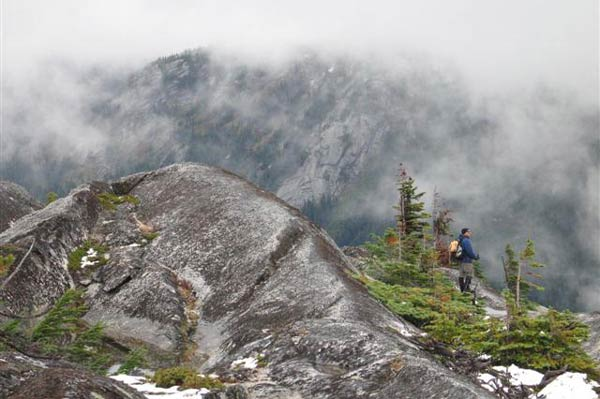
\includegraphics[scale=0.4]{bilder/hiking.jpg} & 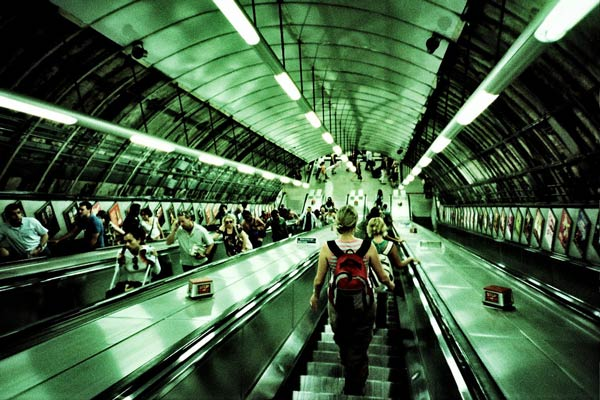
\includegraphics[scale=0.4]{bilder/tube.jpg}\\
			\multicolumn{2}{c}{Quelle: \href{http://hood.ie/}{http://hood.ie/}}
		\end{tabulary}
  		\end{adjustwidth}
	\end{table}

%\\ \\
\noindent
Letztendlich wird die Möglichkeit zur verbindungsunabhängigen Realisierung einer Funktion durch ihren Zweck bedingt. Bei der Entwicklung der Anforderungen kann aber berücksichtigt werden, daß auch für synchrone Interaktions-Funktionalität, wie beispielsweise Instant-Messaging, eine optionale asynchrone Alternative in Form einer verzögerten Nachrichten-Übermittlung, immer noch den zugedachten Zweck erfüllen kann.\\ \\
\noindent
%Seit der Einführung des AppCache-Standards in Html5 
% Seit Ende der 2000-nuller Jahre
In Rahmen des Projekts \textbf{Pumas Voyage}$^{\textbf{\ref{WIKIGOOGMAP}}}$%
% footnote
\addtocounter{footnote}{1}%
\footnotetext{\label{WIKIGOOGMAP}\href{http://ceur-ws.org/Vol-1227/paper33.pdf}{Pumas Voyage - http://ceur-ws.org/Vol-1227/paper33.pdf}; letzter Zugriff: 26.04.2015} werden Konzepte und Werkzeuge für die Beteiligung von Schülern an der Verkehrsraumplanung entwickelt. Die Schüler sollen dabei, mit Hilfe von mobilen Endgeräten und einer darauf ausgeführten Web-Anwendung, ihren auf einer Karte dargestellten Schulweg durch Einträge von markanten Punkten mit einer Bewertung von Sicher/Gut oder Gefährlich/Schlecht, und einem optionalen Kommentar, dokumentieren$^{\textbf{\ref{CMTPUMVOYGEOTAG}}}$%
% footnote
\addtocounter{footnote}{1}%
\footnotetext{\label{CMTPUMVOYGEOTAG}Man könnte diesen Vorgang auch als Verkehrsplanungs-spezifisches Geo-Tagging bezeichnen}.\\
Für die Anzeige der Karte, die als Voraussetzung zur Bearbeitungung von Einträgen gesehen werden kann, ist eine Internet-Verbindung erforderlich. Außerdem ist ein Austausch der Daten mit anderen Benutzern noch nicht implementiert - auf jedem Gerät können nur die darauf gesicherten Daten angezeigt werden. Eine Synchronisation aller Benutzer/System-Daten und deren Anzeige auf allen Endgeräten würde die Anwendung um kollaborative Funktionalität erweitern, mit der es zum Beispiel die Möglichkeit zum unmittelbaren Feedback auf neue Einträge oder Änderungen gäbe. Damit aber keine Netzwerk-Verbindungs-Abhängigkeit entsteht sollte die Synchronisation für den Benutzer transparent durchgeführt werden.\\ \\
%\noindent
%\textbf{Ingress}$^{\textbf{\ref{CMTINGRS}}}$%
% footnote
%\addtocounter{footnote}{1}%
%\footnotetext{\label{CMTINGRS}\href{http://de.wikipedia.org/wiki/Ingress\_\%28Spiel\%29}{Ingress - http://de.wikipedia.org/wiki/Ingress\_\%28Spiel\%29}; letzter Zugriff: 26.04.2015} ist ein Augmented-Reality-/Alternate-Reality-Spiel für mobile Geräte. Das Spiel wird im Freien gespielt, und die Spielwelt wird mit standortbezogenen Daten von realen sich an Gebäuden, Denkmälern und Objekten aufgebaut. Im Spiel existieren zwei Gruppierungen, die mit dem Ziel gegeneinander antreten, möglichst große öffentliche Bereiche unter ihre virtuelle Kontrolle zu bringen.\\ \\
\noindent
Eine Entkopplung von der Netzwerk-Verbindungs-Abhängigkeit muß also durch die Möglichkeit zum lokalen Speichern von Anwendungs-Daten, also auch durch das Vorhalten der für die Nutzung der Software benötigten System-Daten bewerkstelligt werden. Allerdings können aus Gründen der Wartbarkeit und der begrenzten Speicher-Kapazität nicht alle System-Daten am Endgerät gespeichert werden. Es ist daher erforderlich, eine Auswahl bezüglich der vom Benutzer benötigten Daten zu treffen und diese vorzuhalten - im Falle einer kartenbasierten Anwendung müssen dafür beispielsweise die Bild-Dateien für die darzustellenden Karten-Abschnitte vorgeladen werden. Die Vorlade-Auswahl kann mit Hife von aufgabenspezifischen Vorhersage-Algorithmen getroffen werden. Im gegebenen geographischen Kontext können die Vorhersage-Strategien beispielsweise auf Bewegungs-Routen basieren.


%synchron bearbeitung von pois.
%man sieht gkeuch den pi
%man kann auch auf anderen zeichnen 
%spiele, navi 

%%%%%%%%%%%%%%%%%%%%%%%%%%%%%%%%%%%%%%%%%%%%%%%%%%%%%%%%%%%%%%
% VoyageX
%%%%%%%%%%%%%%%%%%%%%%%%%%%%%%%%%%%%%%%%%%%%%%%%%%%%%%%%%%%%%%
\subsection{VoyageX}\label{2_VOYAGEX}
Mit der in dieser Arbeit vorgestellten Web-Anwendung VoyageX sollen nun folgende Funktionen implementiert werden:
\begin{itemize}
  \item Kollaborative Bearbeitung von \texttt{Points of Interest (PoI)} auf einer interaktiven Karte
  \item Interaktion zwischen Benutzern
\end{itemize}
%Im Rahmen dieser Arbeit soll ein Prototyp einer Web-Awendung für kooperatives Geo-Tagging entwickelt werden. In Abschnitt \ref{2_VOYAGEX} folgt eine Beschreibung der gewünschten Funktionen. 
Es müssen in diesem Rahmen aber sowohl weitere Anwendungskomponenten (z.B. ein Benutzersystem) als auch Konzepte zur Benutzerführung (z.B. die Gestaltung von Arbeits-Menus) durch alle benötigten Funktionen entwickelt werden, um die fertige Anwendung testen zu können. Im folgenden werden also auch die Konzepte und Funktionalität dieser Komponenten vorgestellt.
%Mitwirkende Benutzer müssen sich auf der Web-Seite registrieren um die Bearbeitungs-Funktionen nutzen zu können. Nicht
%registrierte Benutzer können nur "`lesend"' auf die Anwendung zugreifen.\\ \\
%\subsection{Funktionsumfang}\label{4_FU}
%\begin{itemize}[leftmargin=*,noitemsep,topsep=1ex,parsep=0pt,partopsep=0pt]
%\item \textbf{plain text}: ein plain-text eintrag besteht nur aus text. allerdings wird als default icion ein %\end{itemize}
%\subsubsection{Darstellung der Karte und positionsbezogener Gestaltungs-Elemente}
\subsubsection{Benutzerverwaltung}
%Die Bearbeitung von Karten und ein öffentlicher Nachrichten-Austausch
In einem kollaborativen Kontext müssen die Aktionen mehrer Benutzer synchronisiert werden. Für VoyageX wird daher ein Benutzer und Autorisierungs-System benötigt.\\
Die Benutzer führen persistente Aktionen aus, deren Ergebnisse im System gespeichert werden, und von allen Benutzern wahrgenommen werden können. Jede Änderung der System-Daten soll dabei einem Benutzer zugeordnet werden können.\\ \\
Für die Realisierung des Benutzer-Systems sind folgende Komponenten erforderlich:
\begin{itemize}
  \item Registrierung
  \item Session-Verwaltung
\end{itemize}
Eine über Einladung gesteuerte Gruppen-Verwaltung wäre sinnvoll und kann je nach Zeitverfügbarkeit optional
implementiert werden.
%Es werden 2 Arten
%email passwort oder facebook
%andere benutzer können jeden sehen
%gruppenverwaltung wäre sinnvoll
%per einladung 

\subsubsection{Darstellung der Karte und Bearbeitungs-Werkzeuge}
%Zur Darstellung einer Karte müssen aus den im vorigen Abschnitt vorgestellten API-Anbietern ein Tile-Service-Provider und ein Map-Viewer gewählt werden. Damit können folgende Grundfunktionen der Karten-Navigation implementiert werden:
In der graphischen Benutzeroberfläche wird eine Landkarte angezeigt. Diese ist interaktiv und es werden
folgende Navigations-Funktionen für die Berarbeitung von PoI-Einträgen implementiert:
\begin{itemize}
  \item Ein Benutzer kann durch "`ziehen"' der Karte, oder durch Eingabe von Koordinaten, jede beliebige Kartenposition im Browser-Fenster anzeigen lassen.
  \item Jeder Kartenausschnitt kann in mehreren Auflösungen (Zoom-Level) angezeigt werden.
  \item Es werden graphische Elemente in der Benutzeroberfläche bereitgestellt, mit denen Punkte auf der Karte optisch gekennzeichnet werden (Markers), sowie zusätzliche Informationen (Popups) zu diesen Markierungen angezeigt werden können.
\end{itemize}
Zur Nutzbarmachung der Bearbeitungsfunktionen von VoyageX werden Menus sowie Werkzeug- und Steuerungs-Elemente bereitgestellt, die dem Benutzer eine schnelle Interaktion und Navigation ermöglichen.

\subsubsection{Erstellen von Einträgen}
Jeder registrierte Benutzer kann neue PoI-Einträge erstellen, indem er auf der Karte einen Punkt markiert und zu diesem über einen Eingabe-Dialog eine Beschreibung oder andere Informationen speichert (Geo-Tagging). Optional kann auch eine Multimedia-Datei an den Eintrag angehängt werden - alle Informationen sollen dann in einem Popup-Fenster über dem Marker des Eintrags angezeigt werden.\\
Alle anderen Benutzer können diese Einträge (als Markers und Popups) sofort$^{\textbf{\ref{CMTPUMVOYGEOTAG}}}$%
% footnote
\addtocounter{footnote}{1}%
\footnotetext{\label{CMTPUMVOYGEOTAG}Oder sobald sie online sind.} ebenfalls auf ihren eigenen Geräten sehen, und weitere Texte und Anhänge hinzufügen.
%Ein Benutzer soll Informationen zu einem ausgewählten Standort speichern können. Neben einem obligatorischen Beschreibungs-Text soll auch eine Multimedia-Datei an die Beschreibung angehängt werden können\\ \\
%Benutzer sollen auch bereits existierende, selbst- oder durch andere Benutzer verfasste Einträge kommentieren können. Auch dabei soll der Anhang einer Multimedia-Anhang erlaubt sein.

\subsubsection{Interaktion (Follow)}
Neben der Bearbeitung von PoI-Einträgen implementiert VoyageX eine Infrastruktur für die Kommunikation zwischen Benutzern. Entfernte Benutzer können mit deren Zustimmung als Kontakte gespeichert werden. Diese bestätigten Kontakte werden auf der Karte mit einem Marker angezeigt, über dessen Funktions-Menu verschiedene Interaktionen gestartet werden können.\\
Im Rahmen der Interaktion zwischen Benutzern sind auch durch Persönlichkeits-Rechte bedingte, besondere Sicherheits-Aspekte zu berücksichtigen. Dafür soll ein Benutzer die Möglichkeit haben, entsprechende Einstellungen vorzunehmen.

\paragraph{Rechteverwaltung}
Jeder Benutzer soll selbst festlegen könne, welche entfernten Benutzer (Peers) mit ihm in Interaktion
treten können.\\
Die Erteilung einer entsprechenden Berechtigung kann nur über eine Anfrage an den gewünschten Interaktions-Partner, und mit seiner Zustimmung erfolgen. Wird die Interaktions-Berechtigung erteilt, kann sie pauschal für alle Aktionen gelten - eine gegliederte Rechteverwaltung kann optional für den Fall ausreichender zeiticher Resourcen implementiert werden.

\paragraph{Benachrichtigungen}
Alle online-Benutzer erhalten unmittelbar Benachrichtigungen zu neuen Einträgen oder Kommentaren, außerdem werden diese auch sofort in der eigenen lokalen Ansicht jedes Benutzers angezeigt.\\ \\
Sofern ein Benutzer die Location-Sharing-Funktion seines Browsers, und im Falle mobiler Endgeräte zusätzlich GPS aktiviert hat, kann er es entfernten Benutzern erlauben, Benachrichtigungen über seine eigenen Standort-Änderungen zu erhalten. Diese Funktion muss in der Anwendung explizit aktiviert bzw. deaktiviert werden.

\paragraph{Kommunikation}
Benutzer haben die Möglichkeit, über Instant Messaging miteinander zu kommunizieren. Dabei sind
folgende Chat-Typen implemetiert:
\begin{itemize}[leftmargin=*,noitemsep,topsep=1ex,parsep=0pt,partopsep=0pt]
\item \textbf{P2P-Chat}: Die ausgetauschten Nachrichten sind nur für 2 Kommunikationspartner sichtbar.
\item \textbf{Konferenz-Chat}: Mehrere Kommunikationspartner können sich am Chat beteiligen.
\end{itemize}
Die Nachrichten werden begrenzt gespeichert, d.h. daß ein Benutzer beim Wiederöffnen eines  geschlossenen Chat-Fensters oder nach dem Neustart der Anwendung einen begrenzten Teil Nachrichten-Historie sehen kann.
Private Nachrichten werden nur von den beiden Kommunikationspartnern jeweils lokal gespeichert. Konferenz-Nachrichten werden zusätzlich im Backend gespeichert, und können so auch nach einem Wechsel auf ein anderes Endgerät angezeigt werden.

\paragraph{Kontrolle entfernter Darstellungs-Elemente}
Jedem Peer ist auf der (lokalen) Karte eines Benutzers ein Marker zugeordnet. 
Eine weitere Form der Interaktion soll nun durch die entfernte Kontrolle eines solchen Markers durch den Peer implementiert werden. Dabei kann der Peer die Position des ihm zugeordneten Markers auf der entfernten Karte steuern. Die Positions-Änderungen des Markers werden dann durch die Darstellung von Verbindungslinien in Form eines Pfades "`aufgezeichnet"'. Auf diese Weise kann sich ein User von einem Peer beispielsweise navigatiorische Hilfestellung geben lassen.

\subsubsection{Funktionsumfang im Offline-Betrieb}
Folgende Dateien und Objekte müssen für die Funktionsfähigkeit der Anwendung im Offline-Betrieb vom Client eines Benutzers lokal gespeichert werden:
\begin{itemize}
  \item Karten-Kachel-Bilder
  \item PoI Einträge und Kommentare
  \item Konferenz- und P2P-Chat Nachrichten
  \item Peer-Daten
\end{itemize}
Allerdings können nicht alle Kachel-Bilder der Weltkarte in allen Auflösungen lokal gespeichert werden.
Das selbe gilt in Bezug auf die kompletten System-Daten. 

\paragraph{Kartenkacheln}
Zur Anzeige von Karten werden einzelne Karten-Kacheln in verschiedenen Maßstäben von einem \texttt{Tile-Service} aus dem Internet geladen, und anschliessend zur Kartenansicht zusammengefügt.\\
%Nachdem aber die Internet-Verbindung nicht immer garantiert ist muß eine Möglichkeit gefunden werden, die benötigten Bild-Dateien auch im Offline-Betrieb in die Kartenanzeige zu integrieren. Dabei sind Lösungen zu finden, 
Für eine Netzwerk-Verbindungs-unabhängige Karten-Darstellung werden folgende Probleme von VoyageX entschieden: 
	\begin{itemize}
		\item welche Bild-Dateien vorab geladen und gespeichert werden% sollen
		%: Dafür muß ein Algorithmus gefunden und implementiert werden, der die vom Benutzer für die Bearbeitung benötigten Karten-Ausschnitte vorhersagt.
		\item wie diese Bild-Dateien lokal gespeichert werden% sollen
		\item wie diese Bild-Dateien dann vom Karten-Viewer eingebunden werden% können
	\end{itemize}
Eine 
\paragraph{POI-Einträge}
Alle POI-Einträge werden im Backend$^{\textbf{\ref{CMTBEREF1}}}$%
% footnote
\addtocounter{footnote}{1}%
\footnotetext{\label{CMTBEREF1}Das Backend wird in Abschnitt \ref{5_BE} ausführlich beschreiben.} gespeichert - lokal können aber wegen der begrenzten Speicher-Kapazität nur bestimmte Einträge gespeichert werden. PoI-Einträge beziehen sich immer auf bestimmte Karten-Positionen, also gilt bei der Entscheidung über die Auswahl der lokal zu speichernden Einträgen das gleiche wie für Karten-Kacheln.\\
Allerdings wird bei Einträgen ein zusätzliches Relevanz-Kriterium eingeführt: vom Benutzer explizit markierte Einträge (Bookmarks) sind jederzeit verfügbar, d.h. daß nicht nur die Bookmark-Information sondern auch der referenzierte Kartenbereich lokal persistent gehalten wird. \\
%werden immer dann mit den system-daten synschronisiert wenn der benutzer online ist.\\
Bookmarks nur lokal gespeichert.





\paragraph{Nachrichten}
Anders als bei POI-Einträgen ist für Chat-Nachrichten kein Karten-Kontext erforderlich. Daher können
diese mit einem einfachen Cache-Algorithmus, beispielsweise einer FIFO-History-Queue, verwaltet werden.

\paragraph{Peer-Daten}
Peer-Daten sind Teil der Information von POI-Einträgen und Chat-Nachrichten, deshalb werden sie für deren vollständige Anzeige benötigt. Peer-Daten sollen sowohl im Backend als auch lokal als eigene Daten-Strukturen gespeichert werden.

\subsubsection{Synchronisation}
Nachdem nun ein Benutzer für einen bestimmten Zeitraum offline war, kann eine Synchronisation
der lokalen Daten mit den System-Daten in folgenden Fällen erforderlich werden:
	\begin{itemize}
		\item der Benutzer hat selbst zwischenzeitlich neue Einträge erstellt, geändert oder gelöscht
		\item andere Benutzer haben zwischenzeitlich neue Einträge erstellt, geändert oder gelöscht
	\end{itemize}
Sobald der Benutzer nach einer Netzwerk-Verbindungs-Unterbrechung wieder online ist, muß sein Client mit dem Backend einen Daten-Abgleich durchführen. Falls der Benutzer Daten geändert hat muß das Backend alle anderen online-Clients über die Änderungen informieren, damit die Clients wiederum ihr eigenes lokales Cache synchronisieren können.




\newpage
%%%%%%%%%%%%%%%%%%%%%%%%%%%%%%%%%%%%%%%%%%%%%%%%%%%%%%%%%%%%%%
%
% Kapitel 3: Existierende Lösungen
%
%%%%%%%%%%%%%%%%%%%%%%%%%%%%%%%%%%%%%%%%%%%%%%%%%%%%%%%%%%%%%%
%\newgeometry{textheight=257mm}
\enlargethispage{3\baselineskip} % allow 3 more lines on current page

\section{Anforderungen und Existierende Lösungen}
Nach einem Überblick über Grundlagen und Entwicklung ortsbezogener Anwendungen in den Abschnitten \ref{3_GRUNDL} und \ref{3_LBSN} werden die Funktionen einiger existierender Anwendungen beschrieben und miteinander verglichen (Abschnitte \ref{3_UEBER} und \ref{3_ANW}) und dann auf die Anwendungsfälle von VoyageX abgebildet. Das Kapitel schliesst mit einer Zusammenstellung von Web Mapping APIs (Abschnitt \ref{3_WEBMAPAPIS}).

%%%%%%%%%%%%%%%%%%%%%%%%%%%%%%%%%%%%%%%%%%%%%%%%%%%%%%%%%%%%%%
% Grundlagen
%%%%%%%%%%%%%%%%%%%%%%%%%%%%%%%%%%%%%%%%%%%%%%%%%%%%%%%%%%%%%%
\subsection{Grundlagen ortsbezogener Anwendungen}\label{3_GRUNDL}

\subsubsection{Geo-Informations-Systeme und Kartendienste}
Ein Geo-Informations-System (GIS) ist ein System zur Erfassung, Speicherung,  Bearbeitung, Analyse, Organisation und Präsentation für jede Art von räumlicher oder geographischer Information.\cite{GIS:WIKIDEF} \\
GIS bilden mit ihren Funktionen, Daten und Modellen die Grundlage für die Erstellung von Kontext-bezogenen Karten. Die verschiedenen GIS-Standards werden vom Open Geospatial Consortium$^{\textbf{\ref{CMTOGC}}}$%
% footnote
\addtocounter{footnote}{1}%
\footnotetext{\label{CMTOGC}\href{http://www.opengeospatial.org/}{OGC - http://www.opengeospatial.org/}; letzter Zugriff: 23.04.2015} (OGC) entwickelt, und ermöglichen die Realisierung von unterschiedlichen \texttt{GIS-Anwendungen}, darunter die auf Kartendiensten aufbauende \texttt{Web-Mapping}-Projekte wie Google$^{\textbf{\ref{WIKIGOOGMAP}}}$%
% footnote
\addtocounter{footnote}{1}%
\footnotetext{\label{WIKIGOOGMAP}\href{http://de.wikipedia.org/wiki/Google_Maps}{http://de.wikipedia.org/wiki/Google\_Maps}; letzter Zugriff: 26.02.2015}
, Bing$^{\textbf{\ref{WIKIBINGMAP}}}$%
% footnote
\addtocounter{footnote}{1}%
\footnotetext{\label{WIKIBINGMAP}\href{http://en.wikipedia.org/wiki/Bing_Maps}{http://en.wikipedia.org/wiki/Bing\_Maps}; letzter Zugriff: 26.02.2015}
oder OpenStreetMaps$^{\textbf{\ref{WIKIWEBMAP}}}$%
% footnote
\addtocounter{footnote}{1}%
\footnotetext{\label{WIKIWEBMAP}\href{http://en.wikipedia.org/wiki/Geographic_information_system\#Applications}{http://en.wikipedia.org/wiki/Geographic\_information\_system\#Applications}; letzter Zugriff: 26.02.2015}  
.

  \begin{figure}
      \centering
	  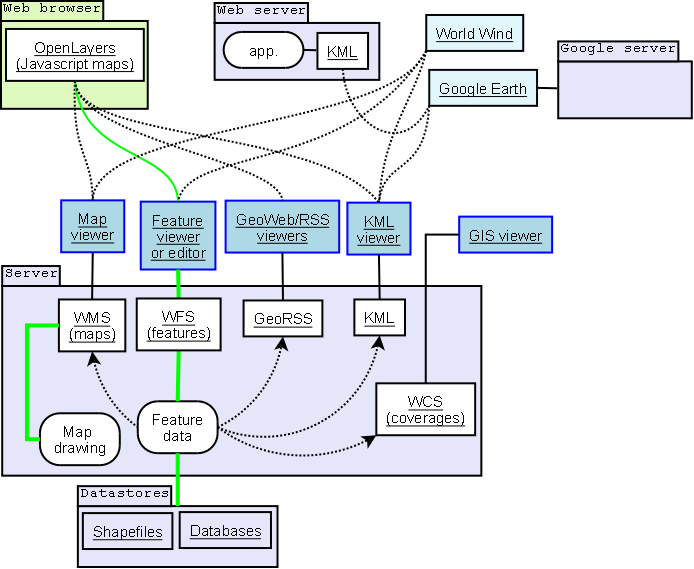
\includegraphics[scale=0.3]{bilder/Geoservices_server_with_apps.png}\\ \vspace{0.8cm}
  	  \caption{Vernetzung von GIS-Werkzeugen durch OGC Standards.\newline Quelle: wikipedia}
  \end{figure}

\subsubsection{Location Based Services (LBS)}
In den 1990ern wurde mit dem Active Badge System$^{\textbf{\ref{ATTACTBADG}}}$ das erste Endgerät zur personellen Lokalisierung entwickelt.
Im folgenden wurden durch die Integration von Positionsbestimmungs-Systemen in die zunehmend verbreiteten Mobil-Funk-Geräte die technischen Voraussetzungen für die Entwicklung von Anwendungen im Kontext standortbezogener Dienste für einen Massen-Markt geschaffen.\\
Wie bei vielen sozio-technischen Entwicklungen konnten hier verschiedene Anwendungsbereiche aus der Informations-Technologie auf nahezu selbstverständliche Weise zusammengefügt werden. Und aus dieser Zusammenfügung sind wiederum neue Anwendungsbereiche entstanden.

\paragraph{Anwendungsbereiche}\label{sec:GL:GEOTAG}
Naheliegendes Anwendungsgebiet für eine verbreitete Nutzung von LBS sind offensichtlich Kartendienste oder Webseiten und Anwendungen aus dem Bereich Tourismus. Die rein sachlichen Informationen zu geographischen Punkten werden hierbei oft auch mit subjektive Erfahrungsberichten ergänzt.\\
%, aus denen auch Crowd-Based-Recommender-System aufgebaut werden kann.\\
Auf die Nutzung von LBS in Sozialen Netzwerke wird in Abschnitt \ref{2_LBSN} näher eingegangen.\\
Geo-basierte Dienste werden auch von Spiele-Web-Seiten und Apps genutzt, wobei in der Regel auch eine soziale Community um das Spiel entsteht. Als Beispiel sei hier Ingress$^{\textbf{\ref{WIKIINGRESS}}}$%
% footnote
\addtocounter{footnote}{1}%
\footnotetext{\label{WIKIINGRESS}\href{http://de.wikipedia.org/wiki/Ingress_(Spiel)}{http://de.wikipedia.org/wiki/Ingress\_(Spiel)}; letzter Zugriff: 03.04.2015}
gegeben, wobei es darum geht, reale Gebiete im virtuellen Raum zu erobern.

\paragraph{Geo-Tagging}\label{sec:GL:GEOTAG}
Geo-Tagging ist eine Assoziation geographischer Positions-Daten mit einem Kontext aus Objekten (Gebäude, Stelle an einem Fluss, ...), Ereignissen (Konzert, ...), Personen oder Zuständen (Wetter, ...). Diese Assoziation kann aus 2 Perspektiven betrachtet werden:
\begin{itemize}[leftmargin=*,noitemsep,topsep=1ex,parsep=0pt,partopsep=0pt]
\item Zu einem bekannten Ort sollen Informationen ausgegeben werden
\item Zu einem bekannten Objekt oder Ereignis oder Person soll der Ort ausgegeben werden, wobei dieser zeitabhängig sein kann.
\end{itemize}
Durch die beliebig große Kontext-Auswahl kann aus einer einzelnen geographischen Ortsangabe eine Vielzahl von Diensten entwickelt werden.


\paragraph{Adaptive Systeme: Context Awareness und Social Awareness}
Bei adaptiven Systemen wird die Ausführung von Aufgaben mit impliziten Informationen über den Benutzer parametrisiert. Diese Parameter werden durch das Verhalten oder andere Faktoren aus dem Benutzerumfeld
abgeleitet.\\ 
"`Kontext ist jede Information, die zur Beschreibung einer Situation von Personen, Orten oder Objekten genutzt werden kann, und dabei für die Interaktion zwischen einem Anwendungsbenutzer und der Anwendung relevant ist. Ein System ist Kontextsensitiv, wenn es einem Benutzer Informationen liefert die er für das Lösen einer Aufgabe  nutzen kann."'\cite{COMPASS:AH}\\
"`Soziale Wahrnehmung ist generelles Wissen über andere in einem sozialen oder kommunikativen Kontext. Sie offenbart das Vorhandensein von Aufmerksamkeit oder Interesse bei den Beteiligten."'\cite{UNIGE:KOA}

\paragraph{Crowdsourcing}
Crowdsourcing ist eine im Rahmen der Web-2.0 Entwicklung entstandene, gegebenenfalls anonyme Form der Kooperation, bei der die Benutzer eines Netzwerks oder einer Community dessen Wert und Nutzen durch eigene Beiträge generieren. Die soziale Wahrnehmung kann dabei eine qualitätssichernde und -fördernde Wirkung entfalten, und die Leistungsfähigkeit eines durch Crowdsourcing entstandenen adaptiven Systems deutlich steigern.
%Die Nutzer schaffen dabei in Eigenregie ein auf sie selbst zugeschnittenes 

\enlargethispage{3\baselineskip} % allow 3 more lines on current page
%%%%%%%%%%%%%%%%%%%%%%%%%%%%%%%%%%%%%%%%%%%%%%%%%%%%%%%%%%%%%%
% Location Based Social Networks
%%%%%%%%%%%%%%%%%%%%%%%%%%%%%%%%%%%%%%%%%%%%%%%%%%%%%%%%%%%%%%
\subsection{Location Based Social Networks (LBSN)}\label{3_LBSN}
"`Ein LBSN bedeutet nicht nur das Hinzufügen von Ortsangaben zu einem bestehenden sozialen Netzwerk damit die Benutzer ortsbezogene Informationen teilen können. Es werden dabei auch neue soziale Strukturen erschaffen die Benutzer sowohl auf Grund ihrer Nähe in der realen Welt, aber auch wegen gemeinsamer, durch Geo-Tags erkennbare Interessen und Aktivitäten zusamenführt."'\cite{ZHENG:LBSNTUT}\\ \\
% erreichen bei weitem nicht mehr die Benutzerzahlen von 2010-2012.
%Im Rahmen des P3-System-Projekts wurde Benutzer-Anforderungen für LBSNs analysiert\cite{[S. 38-46]JONGRAN:P3SYS}. Die Befragten wünschten sich:
%\begin{itemize}[leftmargin=*,noitemsep,topsep=1ex,parsep=0pt,partopsep=0pt]
%\item Ad-Hoc Interaktion mit Freunden, Familie, Kollegen aber auch Fremden
%\item Informationen über die Beliebtheit und Nutzung öffentlicher Resourcen
%\item Unterstützung bei der VerteiAufgabenverteilung
%\end{itemize}
Anwendungen, in denen Ortsangaben geteilt werden (Location Sharing Applications), können grob in 2 Kategorien
eingeteilt werden \cite{LINETAL:4SQ}:
\begin{itemize}[leftmargin=*,noitemsep,topsep=1ex,parsep=0pt,partopsep=0pt]
\item zweck-bezogen: Benutzer fragen aktiv nach Informationen zu den Aufenthaltsorten anderer Benutzer
\item sozial-bezogen: Benutzer teilen ihren eigenen Aufenthaltsort anderen Benutzern (Freunden) mit
\end{itemize}

\begin{table}
  \centering
  \begin{tabulary}{\columnwidth}{| >{\centering}m{1.5cm} | L |}
  \hline
    1989-93 & Active Badge System – beginning of personal mobile positioning \\ \hline
    ... &  \\ \hline
    1999 & The first Digital Location Based Service Patent was filed in the US \\ \hline
    1999 & The first consumer LBS-capable mobile web device was the Palm VII \\ \hline
    2000 & After approval from the world\'{e}s 12 largest telecom operators, Ericsson, Motorola and Nokia jointly formed and launched the Location Interoperability Forum Ltd \\ \hline
    2000 & Launch of Dodgeball – The first location-based social network for mobile devices (Acquired by Google in 2005) \\ \hline
    2001 & The first LBS services were launched by TeliaSonera in Sweden (FriendFinder, yellow pages, houseposition, emergency call location etc.) and by EMT in Estonia (emergency call location, friend finder, TV game) \\ \hline
    2001 & The first commercial LBS service in Japan was launched by DoCoMo, based on triangulation for pre-GPS handsets \\ \hline
    2002 & Go2 and AT\&T Mobility launched the first (US) mobile LBS local search application that used Automatic Location Identification (ALI) technologies mandated by the FCC \\ \hline
    2004 & Where, Plazes \\ \hline
    2005 & Sociallight, Loopt, Limbo \\ \hline
    2005 & Google acquires Dodgeball \\ \hline
    2006 & Itsmy.com, Gypsii \\ \hline
    2007 & The launch of iPhone \\ \hline
    2007 & Gowalla, BrightKite, Qyoe, Tupalo.com \\ \hline
    2009 & Whrrl, TellMeWhere, FireEagle, Moximity \\ \hline
    2009 & Locassa, Foursquare \\ \hline
    2009 & Twitter adding location feature \\ \hline
    2009 & Google turn Dodgeball into Google Latitude \\ \hline
    2010 & Google Places, SCVNGR, Yelp, Skout, Friendticker \\ \hline
    2011 & Facebook check-ins \\ \hline
    2012 & Apple Maps, Google Glass Project \\ \hline
  \end{tabulary}
  \caption{Entwicklung von Applikationen mit Nutzung ortsbezogener Dienste$^{\textbf{\ref{GEOA1}}}$ \newline Quelle: geoawesomeness}
\end{table}
\addtocounter{footnote}{1}
\footnotetext{\label{GEOA1}\href{http://geoawesomeness.com/knowledge-base/location-based-services/location-based-services-chronology/}{geoawesomeness}; letzter Zugriff: 23.02.2015}  


\subsubsection{Check-In}
Ludford et al. haben Studien zur Bereitschaft von Sharescape$^{\textbf{\ref{WIKIGOOGMAP}}}$%
% footnote
\addtocounter{footnote}{1}%
\footnotetext{\label{WIKIGOOGMAP}\href{http://experts.umn.edu/pubDetail.asp?t=pm\&id=70049112551}{Sharescape - http://experts.umn.edu/pubDetail.asp?t=pm\&id=70049112551}; letzter Zugriff: 26.02.2015}-Anwendungs-Benutzern zur Veröffentlichung ihrer aktuellen Aufenthaltsorte durchgeführt, und dabei herausgefunden, daß in erster Linie private Orte wie "`zu  Hause"' oder auch der Arbeitsplatz geschützt werden sollten.\cite{LUETAL:CSULPI}\\ \\
Die Bekanntgabe des eigenen Aufenthaltsortes im öffentlichen Raum erfreute sich aber spätestens dann großer Beliebtheit, seit diese als \texttt{Check-In} Funktion bei Foursquare$^{\ref{4SQU}}$ angeboten wurde. Ein Check-In wird dabei aktiv vom Benutzer initiert. Diese Information
wird im System gespeichert, und kann optional an die vom Benutzer autorisierten Kontakte weitergegeben oder aber auch über andere soziale Netzwerk-Dienste wie Twitter oder Facebook veröffentlicht werden.
Check-Ins werden als Beitrag zum Gemeinschafts-Gefühl (Community-Experience) meistens belohnt, dies kann sowohl virtuell z.B. durch Vergabe von Badges oder aber auch real z.B. durch Gewährung eines Rabatts vom Lokal in dem sich der Benutzer gerade befindet.\\
Einige "`Social Networks"' waren sogar mit einem Angebot, das fast ausschließlich aus personalisierten Geo-Tagging Informationen, außerordentlich erfolgreich, mittlerweile scheint jedoch der Höhepunkt dieser Entwicklung überschritten zu sein, und positionsbezogene Dienste werden zunehmend "`nur"' als Ergänzung zu den originären Angeboten eines Sozialen Netzwerks genutzt.


\subsubsection{Recommender Systems}\label{2_RECSYS}
Ein Empfehlungsdienst (englisch Recommender System) ist ein Softwaresystem welches das Ziel hat eine Vorhersage zu treffen, die quantifiziert wie stark das Interesse eines Benutzers an einem Objekt ist, um dem Benutzer genau die Objekte aus der Menge aller vorhandenen Objekte zu empfehlen, für die er sich wahrscheinlich am meisten interessiert. \cite{RECSYS:WIKIDEF}\\ \\
Recommender Systems sind Adaptive Systeme die sowohl ideele wie auch kommerzielle Ziele verfolgen
in dem sie den Benutzer eine Auswahl von kontextueller Information zukommen lassen.
Verschiedene Vorhersage-Strategien zur Priorisierung dieser Informationen sind nach \cite{COMPASS:AH}: 
\begin{itemize}[leftmargin=*,noitemsep,topsep=1ex,parsep=0pt,partopsep=0pt]
\item Soziale Filterung
\item Case-Based Reasoning (CBR)
\item Item-Item Filtering
\item Category Learning
\end{itemize}
%prioritäte einer information (zb pois) fr einen nutzer
%zu bewerten.
%Used prediction methods include social filtering [12], case-based reasoning (CBR) [11], item-item filtering %[5] and category learning [13]
Bei LBS kommt ein harter Fakt hinzu, der die Auswahl wesentlich erleichtert. Die Kenntnis über den Aufenthaltsort eines Nutzers begrenzt die Auswahl relevanter Information nicht nur geographisch, sondern auch inhaltlich - abhängig vom Angebot der aktuellen Umgebung.

%\subsubsection{Wirtschaft und Konsum}
%Shops

%\subsubsection{Kultur und Freizeit}
%Food, Drink, Music, Theatre, Dating

%\subsubsection{Sehenswürdigkeiten und Routenplanung}
%Travel/Tourist

%%%%%%%%%%%%%%%%%%%%%%%%%%%%%%%%%%%%%%%%%%%%%%%%%%%%%%%%%%%%%%
% Überblick
%%%%%%%%%%%%%%%%%%%%%%%%%%%%%%%%%%%%%%%%%%%%%%%%%%%%%%%%%%%%%%
\subsection{Überblick und Vergleich}\label{3_UEBER}
Neben den von allen Anwendungen angebotenen allgemeinen Grundfunktionen bietet jede App noch Zusatzfunktionen die aus ihrem charakteristischen Kontext abgeleitet werden.\\
In der nachstehenden Matrix sollen allgemeine und charakteristische Funktionen aufgezählt und voneinander abgegrenzt werden, um einen Vergleich des Funktionsumfangs von VoyageX mit jenem anderer Produkte zu ermöglichen. Die Anzahl der angebotene Funktionen soll aber kein alleiniges Qualitäts-Kriterium für diese Arbeit  darstellen, da es bei VoyageX weniger um die Entwicklung eines neuartigen Konzepts als vielmehr um die Technische Realisierung von Kooperation und adaptiver Synchronisation gehen soll.
	\begin{table}[H]
	\begin{adjustwidth}{-0,3cm}{0,3cm}
		\centering
		\begin{tabulary}{18cm}{|L|C|C|C|C|C|C|C|C|C|C|C|C|C|C|C|C|C|}
		\hline
			 & \textbf{1} & \textbf{2} & \textbf{3} & \textbf{4} & \textbf{5} & \textbf{6} & \textbf{7} & \textbf{8} & \textbf{9} & \textbf{10} & \textbf{11} & \textbf{12} & \textbf{13} & \textbf{14} & \textbf{15} & \textbf{16} & \textbf{17} \\ \hline
%						  1   2   3	  4   5   6   7   8   9   10  11  12  13  14  15  16  17
			VoyageX     & X & X & - & - & X & - & - & X & X & X & - & - & - & X & X & X & X \\ \hline
			Foursquare  & X & X & X & X & - & - & X & X & X & - & X & - & - & - & - & - & - \\ \hline
			Swarm	    & X & X & - & X & - & X & X & X & X & X & X & X & - & X & - & - & - \\ \hline
			Path/Talk 	& X & X & - & - & - & - & - & X & X & X & X & X & X & X & - & - & - \\ \hline
			Yelp        & X & X & X & X & - & - & - & X & - & X & X & - & - & - & - & - & - \\ \hline
			TripAdvisor & X & X & X & X & - & - & - & X & - & - & - & - & - & - & - & X & - \\ \hline
		\end{tabulary}
	\caption{Abgrenzung des Funktionsumfangs}{
\vspace{0.2cm}
\begin{enumerate}[labelwidth=0pt,leftmargin=39pt,noitemsep,topsep=0pt,parsep=0pt,partopsep=0pt]
\item PoI - Eintragen (M)obile, (PC), (X)...Any
\item PoI - Kommentieren / Review
\item PoI - Suche nach Kategorien/Tags
%\item PoI - Check In
\item PoI - Bewertung für PoI und/oder Kommentar
\item PoI - Echtzeit-Benachrichtigung bei neuem PoI oder Kommentar
\item Deals Discovery 
\item Belohnung / Badges / Incentives als Motivation für Benutzer
\item Social - Follow-Funktion, Verwaltung und Suchen von Kontakten
\item Social - Location-Sharing / Check In
\item Social - Chat
% TODO yes or no?
% \item Social - Posts
\item Social - Verknüpfung mit Social-Websites
\item Social - Timeline
\item Social - Treffpunkt Planer
\item Social - Echtzeit-Benachrichtigung über Aktivitäten von Kontakten
\item Kontrolle von Darstellungselementen auf entfernten Karten
\item Offline-Anzeige
\item Offline-Bearbeitung
\end{enumerate}
}
	\end{adjustwidth}
	\end{table}

%\restoregeometry

%%%%%%%%%%%%%%%%%%%%%%%%%%%%%%%%%%%%%%%%%%%%%%%%%%%%%%%%%%%%%%
% Anwendungen
%%%%%%%%%%%%%%%%%%%%%%%%%%%%%%%%%%%%%%%%%%%%%%%%%%%%%%%%%%%%%%
\subsection{Anwendungen}\label{3_ANW}

\subsubsection[Foursquare]{Foursquare$^{\textbf{\ref{4SQU}}}$}
% footnote
\addtocounter{footnote}{1}%
\footnotetext{\label{4SQU}\href{https://de.foursquare.com/}{Foursquare - https://de.foursquare.com/}; letzter Zugriff: 22.01.2015}
Foursquare war ein standortbezogenes soziales Netzwerk, welches hauptsächlich durch Software für Mobiltelefone und Smartphones funktioniert. Inzwischen ist es nur noch ein Katalog für Orte. Die Soziale Komponente wurde in die neue App Swarm$^{\textbf{\ref{Swarm1}}}$ verlegt.\cite{4SQ:WIKIDEF}\\
Nach dem Launch der Seite im März 2009 haben sich bis Dezember 2010 bereits 5 Millionen User registriert, und im April 2012 konnten sogar 20 Millionen User gezählt werden. Damit zählt Foursquare zu den erfolgreichsten LBSNs.\\ \\
Location-Sharing bei Foursquare funktioniert über Check-Ins. Dabei muß es sich bei der Check-In-Location um
einen öffentlichen und registrierbaren Ort, also ein Restaurant, Kino oder aber ein öffentliches und registrierbares Ereignis wie besipielsweise ein Konzert oder Festival, handeln.
Wenn ein Benutzer einen Check-In bekannt gibt, wird er von der Anwendung über weitere Orte und Personen in der Umgebung informiert. Benutzer können wiederum das System über neue Locations informieren.\\
Der aktuelle Aufenthaltsort wird bei einem Check-In in einer Historie gespeichert. Wenn 
ein Benutzer häufiger als andere Check-Ins an einem Ort durchführt wird er als Mayor gelistet.\\ \\
Seit der Ausgliederung sozialer Funktionen in die im folgenden Abschnitt beschriebene Swarm-App hat
sich Foursquare-App nun primär auf Crowd-Based-Personal-Recommender-Funktionen spezialisiert. Dabei werden sowohl die Bewertungen von Locations durch alle Benutzer also auch die eigenen Vorlieben als Grundlage
von Empfehlungen von Locations herangezogen.\\ \\
Wie Foursquare bietet auch VoyageX die Funktion, Informationen zum aktuell über GPS ermittelten Standort im System zu speichern.

\subsubsection[Swarm]{Swarm$^{\textbf{\ref{Swarm1}}}$}
% footnote
\addtocounter{footnote}{1}%
\footnotetext{\label{Swarm1}\href{https://www.swarmapp.com/}{Swarm - https://www.swarmapp.com/}; letzter Zugriff: 22.01.2015}
Für die Suche nach einem bestimmten Orten wird nun also weiterhin Foursquare genutzt - Informationen über Kontakte werden mit Swarm gefunden. Eine grundlegende Änderung gegenüber Foursquare ist es, das Teilen von Aufenthaltsinformationen nicht mehr an registrierte Orte zu koppeln. Aus diesem Grund wurde die Check-in-Funktion von Foursquare zu der sogenannten Neighbourhood-Sharing-Funktion für Swarm erweitert - für den Benutzer sind nun auch Kontakte in geographischer Nähe sichtbar ohne daß diese in einen Ort einchecken müssen. Außerdem können Benutzer mit Swarm auch  Orte für zukünfitige Treffen verabreden.\\ \\
Öffentliche Orte werden in Swarm zwar angezeigt, allerdings werden diese von der Foursquare-Datenbank übernommen. Eine derartige funktionale Trennung sorgt für kompaktere Einzel-Apps und erleichtert damit deren jeweilige Bedienbarkeit.

\subsubsection[Path]{Path$^{\textbf{\ref{PATH}}}$ / Talk$^{\textbf{\ref{TALK}}}$}
% footnote
\addtocounter{footnote}{1}
\footnotetext{\label{PATH}\href{https://path.com/}{Path - https://path.com/}; letzter Zugriff: 22.01.2015}
% footnote
\addtocounter{footnote}{1}
\footnotetext{\label{TALK}\href{https://path.com/talk}{Talk - https://path.com/talk}; letzter Zugriff: 22.01.2015}
Path ist eine Social App zum teilen und austauschen vielfältiger Informationen, dazu gehören
\begin{itemize}[leftmargin=*,noitemsep,topsep=1ex,parsep=0pt,partopsep=0pt]
\item Location-Sharing-Infos/Check-Ins
\item Media-Dateien
\item Posts und persönliche Nachrichten
\item Aktivitäten
\item Bewertungen in Form von Emotions (better than Likes)
\end{itemize}
Zum selektiven Teilen stehen dem Benutzer verschiedene Kontakt und Gruppen-Verwaltungs-Funktionen zur Verfügung.\\ \\
Als weiteres Feature werden für jeden Benutzer Informationen zu persönlichen Aufenthalten und Ereignissen in Form einer Timeline gespeichert.\\ \\
Für die Interaktion mit Kontakten wurde mit Talk eine eigene Instant-Messaging-App geschaffen, die aus Path oder aber auch separat gestartet werden kann. Neben den Kommunikations-Funktionen wie Personal- und Group-Chat bietet sie auch eine Neighbourhood-Sharing-Funktion, also eine Benachrichtigung über Kontakte in geographischer Nähe. 

\subsubsection[Yelp]{Yelp$^{\textbf{\ref{YELP}}}$}%
% footnote
\addtocounter{footnote}{1}
\footnotetext{\label{YELP}\href{http://www.yelp.com/about}{Yelp - http://www.yelp.com/about}; letzter Zugriff: 26.01.2015}
Yelp startete ursprünglich als Benutzer-basiertes-Empfehlungs-Portal, und hat sich mittlerweile zu einem Socialen Netzwerk mit entsprechenden Funktionen, also Benutzerprofilen, Freunde-Verwaltung, Nachrichten-Austausch und Follow-Funktion, weiterentwickelt.\\ \\
Im Konzept von VoyageX ist keine Empfehlungs-Funktion vorgesehen, Yelp soll an dieser Stelle vor allem als beispielhafte Anwendung für einen weiteren Anwendungs-Bereich Geo-basierter Dienste erwähnt sein.

\subsubsection[TripAdvisor]{TripAdvisor$^{\textbf{\ref{TRIPADV}}}$}%
% footnote
\addtocounter{footnote}{1}
\footnotetext{\label{TRIPADV}\href{http://www.tripadvisor.de/}{TripAdvisor - http://www.tripadvisor.de/}; letzter Zugriff: 26.01.2015}
TripAdvisor ist ein Beispiel für eine Recommender-Anwendung aus dem Tourismus-Bereich. Im Vergleich zu anderen geo-basierten Recommender-Systemen werden hier aber nicht nur Empfehlungen aus verschiedenen Kategorien für die nähere Umgebung des aktuellen Benutzer-Standorts gegeben, sondern dem Konzept der Seite/App entsprechend auch für Reiseziele in der ganzen Welt.\\
Grundlage für Empfehlungen sind unter anderem die Benutzer-basierten 1-5 Sterne Benotungen der Reise-Orte. Diese Bewertungen werden auch hier wiederum selbst von Benutzern bewertet, wobei auch alle anderen Feedbacks eines Benutzers eingesehen werden können. Ein Möglichkeit zur direkten Kontaktaufnahmen unter Benutzern ist nicht verfügbar, ebensowenig eine sonstige soziale Verknüpfung wie zum Beispiel eine Follow-Funktion. Als einziges soziales Kommunikations-Feature kann bei TripAdvisor ein Forum genutzt werden. Dem Seitenkonzept entsprechend sind auch Funktionen zur direkten Buchung von Hotels oder Flügen in die Anwendung integriert.\\ \\
Ein Feature daß auch für VoyageX interessant wäre, ist die Möglichkeit zum Download von Informationen über ausgewählte Orte für eine spätere Offline-Nutzung. Allerdings werden bei TripAdvisor nur Städte-Informationen zum Download angeboten, eine vollständige Reise-Route kann also nicht bezogen werden.\\
Ein enstprechendes Feature für VoyageX könnte so aussehen:\\
Ein Benutzer kann einen Pfad auf der Karte "`zeichnen"' für den VoyageX dann alle benötigten Kacheln und die im dargestelletn Gebiet eingetragenen POIs speichert. Alternativ könnte auch Pfad als äußere Begrenzung des zu speichernden Gebiets gezeichnet werden.
Dieses Feature ist für VoyageX aber optional, bei ausreichenden zeitlichen Resourcen wird es implememtiert.

%%%%%%%%%%%%%%%%%%%%%%%%%%%%%%%%%%%%%%%%%%%%%%%%%%%%%%%%%%%%%%
% Anwendungsfälle für VoyageX
%%%%%%%%%%%%%%%%%%%%%%%%%%%%%%%%%%%%%%%%%%%%%%%%%%%%%%%%%%%%%%
\subsection{Anwendungsfälle für VoyageX}\label{4_UC}

%\subsubsection{Actors}
%%\begin{enumerate}[labelwidth=0pt,leftmargin=39pt,noitemsep,topsep=0pt,parsep=0pt,partopsep=0pt]
%\begin{itemize}[leftmargin=*,noitemsep,topsep=1ex,parsep=0pt,partopsep=0pt]
%\item \textbf{Benutzer}: Der lokale Benutzer in einem initiierenden Zustand
%\item \textbf{Wahrnehmer}: Der lokale Benutzer in einem induzierten Zustand
%\item \textbf{Peer}: Ein anderer / entfernter Benutzer
%\item \textbf{Comm}: Die Kommunikations-Schicht
%\item \textbf{Backend}: Die Synchronisations-Schicht
%\end{itemize}

\subsubsection{Rolle \textbf{Benutzer}}
Dieser Actor ist der lokale Benutzer, der auf seinem Endgerät mit der Anwendung aktiv arbeitet, also die Bedienungs- und Werkzeug-Elemente der Anwendung benutzt.\\
	%\begin{table}[label=usecases-benutzer,h!]
	\begin{table}[H]\label{usecases-benutzer}
		\centering
		\begin{tabulary}{\linewidth}{|>{\centering}m{1cm}|L|C|C|C|C|C|}
		\hline
			\textbf{Ref} & \textbf{Name} & \textbf{online} & \textbf{offline} & \textbf{synchron} & \textbf{asynchron} & \textbf{visibility} \\ \hline
			\ref{subsubsec:uc_reg} & Registrieren & y & n & y & n & - \\ \hline
			\ref{subsubsec:uc_anm} & Anmelden & y & n & y & n & \# \\ \hline
			\ref{subsubsec:uc_locmapnav} & Lokale Karte navigieren & y & y & y & n & \# \\ \hline
			\ref{subsubsec:uc_remmapnav} & Darstellungs-Elemente auf entfernter Karte steuern & y & n & y & n & \# \\ \hline
			\ref{subsubsec:uc_poinew} & PoI markieren & y & y & y & y & + \\ \hline
			\ref{subsubsec:uc_poinote} & PoI kommentieren & y & y & y & y & + \\ \hline
			\ref{subsubsec:uc_locnote} & Ort merken (Bookmark/Notiz) & y & y & n & n & - \\ \hline
			\ref{subsubsec:uc_reqmefollowpeer} & "`Folgen"' beantragen & y & y & y & y & \# \\ \hline
			\ref{subsubsec:uc_grantpeerfollowme} & "`Folgen"' erlauben & y & y & y & y & \# \\ \hline
% wird vom nächsten usecase-block erfasst
%			Aktionen anderer Benutzer wahrnehmen & y & n & y & y & \# \\ \hline
			\ref{subsubsec:uc_usernote} & Notiz zu anderem Benutzer erstellen & y & y & n & n & - \\ \hline
			\ref{subsubsec:uc_chatp2p} & P2P-Chat & y & y & y & y & \# \\ \hline
			\ref{subsubsec:uc_chatconf} & Konferenz & y & y & y & y & \# \\ \hline
		\end{tabulary}
	\caption{Benutzer-Use-Cases}
	\end{table}
\begin{itemize}[leftmargin=*,noitemsep,topsep=1ex,parsep=0pt,partopsep=0pt]
\item \textbf{online}: der Anwendungsfall tritt im Online-Modus auf.
\item \textbf{online}: der Anwendungsfall tritt im Offline-Modus auf.
\item \textbf{synchron}: Die Daten und Aktionen auf dem lokalen System können in Echtzeit mit dem Backend und somit mit allen Online-Benutzern synchronisiert werden, vorausgesetzt das lokale System ist online. 
\item \textbf{asynchron}: Die Daten und Aktionen auf dem lokalen System können asynchron mit dem Backend abgeglichen werden, der Anwendungsfall erfordert keine synchrone Kooperation.
\item \textbf{visibility}: Bezeichnet die Sichtbarkeit von Daten und Wahrnehmung von Aktionen - oder deren kooperativen Character - für andere Benutzer.
%\renewcommand{\labelitemii}{*}
	\begin{itemize}[leftmargin=*,noitemsep,topsep=1ex,parsep=0pt,partopsep=0pt]
	%\begin{itemize}[label={},labelwidth=0pt,leftmargin=24pt,noitemsep,topsep=0pt,parsep=0pt,partopsep=0pt]
\renewcommand{\labelitemii}{\textbf{+}}
		\item \textbf{public}: Die Daten und Aktionen sind für alle Benutzer sichtbar
\renewcommand{\labelitemii}{\textbf{\#}}
		\item \textbf{protected}: Die Daten und Aktionen sind für ausgewählte Benutzer und/oder nur unter bestimmten Bedingungen sichtbar
\renewcommand{\labelitemii}{\textbf{-}}
		\item \textbf{private}: Daten und Aktionen können von anderen Benutzern nicht wahrgenommen werden.
	\end{itemize}
\end{itemize}


\paragraph{Die Rollen \textbf{Wahrnehmer} und \textbf{Peer}}
Wahrnehmer ist die passive Rolle eines Benutzers, in der er über Änderungen des Verbindungs-Zustands, Änderungen der System-Daten oder Aktivitäten anderer Benutzer benachrichtigt wird.\\
Peer bezeichnet den Benutzer in seiner Rolle als entfernter Benutzer und Kontakt eines lokalen Benutzers.\\
	\begin{table}[H]
		\centering
		\begin{tabulary}{\columnwidth}{|>{\centering}m{1cm}|L|C|C|C|C|C|}
		\hline
			\textbf{Ref} & \textbf{Name} & \textbf{online} & \textbf{offline} & \textbf{synchron} & \textbf{asynchron} & \textbf{visibility} \\ \hline
			\ref{subsubsec:uc_watchconnstate} & Änderung des Internetverbindungs-Status & y & y & y & n & - \\ \hline
			\ref{subsubsec:uc_watchgrantmefollowpeer} & Berechtigung zur Wahrnehmung von Aktionen eines anderen Benutzers erhalten & y & n & y & y & \# \\ \hline
			\ref{subsubsec:uc_watchposofpeer} & Position/Bewegung anderer Benutzer im Nahbereich & y & n & y & y & \# \\ \hline
			\ref{subsubsec:uc_watchpoinewornotebypeer} & Neue PoI-Einträge oder -Kommentare & y & n & y & y & \# \\ \hline
			\ref{subsubsec:uc_watchmsgbypeer} & Neue P2P- oder Konferenz-Nachrichten & y & n & y & y & \# \\ \hline
		\end{tabulary}
	\end{table}

\subsubsection{Rolle \textbf{Comm}}
In der Kommunikations-Schicht sind Interaktions-Funktionen implementiert. Nachrichten werden über die Publish / Subscribe Infrastruktur verteilt.\\
	\begin{table}[H]
		\centering
		\begin{tabulary}{\columnwidth}{|L|C|C|C|C|C|}
		\hline
			\textbf{Name} & \textbf{online} & \textbf{offline} & \textbf{synchron} & \textbf{asynchron} & \textbf{visibility} \\ \hline
			Benachrichtigungen über Bewegungsdaten/Standort von Benutzern & y & n & y & n & \# \\ \hline
			Benachrichtigungen über neue PoI-Einträge & y & n & y & n & \# \\ \hline
			P2P- und Konferenz-Chat-Meldungen & y & n & y & n & \# \\ \hline
		\end{tabulary}
	\end{table}

\subsubsection{Rolle \textbf{Backend}}
Das Backend übernimmt Benutzer-Verwaltungs und Synchronisations-Aufgaben. Für das Versenden von System-Nachrichten werden die Funktionen der Kommunikations-Schicht genutzt.\\
	\begin{table}[H]
		\centering
		\begin{tabulary}{\columnwidth}{|L|C|C|C|C|C|}
		\hline
			\textbf{Name} & \textbf{online} & \textbf{offline} & \textbf{synchron} & \textbf{asynchron} & \textbf{visibility} \\ \hline
			Synchrone Integration von Daten-Änderungen durch Online-Benutzer & y & n & y & - & \# \\ \hline
			Asynchrone Integration von Daten-Änderungen durch wiederverbundene Offline-Benutzer & y & n & - & y & \# \\ \hline
			Benachrichtigung an Benutzer über eine Anfrage zur Wahrnehmung durch einen anderen Benutzer & y & n & y & y & \#  \\ \hline
			Benachrichtigung an Benutzer über Erlaubnis zur Wahrnehmung eines anderen Benutzers & y & n & y & y & \#  \\ \hline
		\end{tabulary}
	\end{table}

%%%%%%%%%%%%%%%%%%%%%%%%%%%%%%%%%%%%%%%%%%%%%%%%%%%%%%%%%%%%%%
% Web Mapping APIs
%%%%%%%%%%%%%%%%%%%%%%%%%%%%%%%%%%%%%%%%%%%%%%%%%%%%%%%%%%%%%%
\subsection{Web Mapping APIs}\label{3_WEBMAPAPIS}
Bibliotheken und Werkzeuge für die Anzeige und Bearbeitung von Karten werden in der Regel von externen Anbietern geliefert.

\subsubsection{Web Mapping Services}
Die meisten Anwendungen nutzen frei verfügbare Online-Kartendienste (Web Mapping Services) zur Darstellung von Karten in der Benutzeroberfläche. Über die Service-APIs sind die Kartenrohdaten meist kostenlos erhältlich, für zusätzliche Geo-Coding-Leistungen wie Routenberechnungen gibt es unterschiedliche Limits oder Gebühren.\\
Verbereitete Anbieter sind:
\begin{itemize}
  \item Google-Maps-API$^{\textbf{\ref{GOOGMAPSAPI}}}$
% footnote
\addtocounter{footnote}{1}
\footnotetext{\label{GOOGMAPSAPI}\href{https://developers.google.com/maps/}{Google Maps API - https://developers.google.com/maps/}; letzter Zugriff: 26.01.2015}:
Google bietet seinen Karten-Dienst seit 2005 an und hat einen großen Anteil an der schnellen Verbreitung
dieser Dienst-Kategorie. Karten können mit unterschiedlichen Ansichts-Typen angezeigt werden, wie zum Beispiel Straßen-Ansicht oder Satelliten-Ansicht.
  \item Bing-Maps$^{\textbf{\ref{BINGMAPSAPI}}}$
% footnote
\addtocounter{footnote}{1}
\footnotetext{\label{BINGMAPSAPI}\href{https://msdn.microsoft.com/en-us/library/dd877180.aspx}{Bing Maps - https://msdn.microsoft.com/en-us/library/dd877180.aspx}; letzter Zugriff: 26.01.2015}
Seit 2010 bietet die Suchmaschine von Microsoft ihren eigenen Kartendienst mit Google-Maps-ähnlichen Funktionen an.
  \item OpenStreetMap$^{\textbf{\ref{OSMMAPS}}}$
% footnote
\addtocounter{footnote}{1}
\footnotetext{\label{OSMMAPS}\href{http://wiki.openstreetmap.org/wiki/Frameworks}{OpenStreetMap- API - http://wiki.openstreetmap.org/wiki/Frameworks}; letzter Zugriff: 26.01.2015}:
OSM ist ein Open-Source-Projekt; demenstprechend gibt es eine Vielzahl von Tools und Frameworks welche die API implementieren und deren Verwendung in einem Projekt unterstützen.
\end{itemize}

\subsubsection{Tile-Service-Providers}
Tile-Services können von einem Web Mapping Service Provider oder aber auch eigenständig angeboten werden. Sie liefern die Bild-Dateien zur Darstellung von Karten in Form von (meistens) 256x256 Pixel großen Kacheln auf denen die zu den GIS-Daten korrespondierenden Karten-Elemente, also Straßen, Gebäude, Flüße, und dgl. angezeigt werden. Die Bild-Dateien können dabei entweder On-The-Fly aus den GIS-Daten generiert, oder vorab aus einem Projektions-Bild extrahiert werden. Zum Download wird eine mit den Koordinaten und dem Zoom-Level parametrisierte URL vom Tile-Service bereitgestellt.\\
Auch für diesen Service gibt es eine großes Spektrum an freien und kommerziellen Anbietern. Als Beispiele für eigenständige Anbieter seien hier folgende angegeben: 
\begin{itemize}
  \item Mapbox$^{\textbf{\ref{MAPB}}}$
% footnotes%
\addtocounter{footnote}{1}%
\footnotetext{\label{MAPB}\href{https://www.mapbox.com/}{Mapbox - https://www.mapbox.com/}; letzter Zugriff: 01.03.2015}%
bietet Download-Kontingente von Free bis einige hundert Euro pro Monat.
  \item MapQuest$^{\textbf{\ref{MAPQ}}}$
% footnote
\addtocounter{footnote}{1}
\footnotetext{\label{MAPQ}\href{http://open.mapquest.de/}{MapQuest - http://open.mapquest.de/}; letzter Zugriff: 26.01.2015}
\end{itemize}

\subsubsection{Map Viewer}
Für die Darstellung von Slippy-Maps LeafletJS$^{\textbf{\ref{FN_SLIPPYM}}}$
% footnote%
\addtocounter{footnote}{1}%
\footnotetext{\label{FN_SLIPPYM}Slippy Map is, in general, a term referring to modern web maps which let you zoom and pan around (the map slips around when you drag the mouse).}
können verschiedene Map Viewer Bibliotheken eingesetzt werden. WMS-API-Provider bieten zwar ihre eigene WMV-APIs an, es gibt aber auch
Drittanbieter wie 
\begin{itemize}
  \item LeafletJS$^{\textbf{\ref{FN_LEAFL}}}$
% footnote%
\addtocounter{footnote}{1}%
\footnotetext{\label{FN_LEAFL}\href{http://leafletjs.com/}{LeafletJS - http://leafletjs.com/}; letzter Zugriff: 01.03.2015}
  \item OpenLayers$^{\textbf{\ref{FN_OPENLAY}}}$
% footnote%
\addtocounter{footnote}{1}%
\footnotetext{\label{FN_OPENLAY}\href{http://openlayers.org/}{OpenLayers - http://openlayers.org/}; letzter Zugriff: 01.03.2015}
  \item JMapViewer{$^{\textbf{\ref{FN_JMAPV}}}$}
% footnote%
\addtocounter{footnote}{1}%
\footnotetext{\label{FN_JMAPV}\href{http://wiki.openstreetmap.org/wiki/JMapViewer}{JMapViewer - http://wiki.openstreetmap.org/wiki/JMapViewer}; letzter Zugriff: 01.03.2015}
\end{itemize}
, welche für die Integration von Karten-Darstellungen in Web-Apps oder native Anwendungen genutzt werden


%\newpage
%%%%%%%%%%%%%%%%%%%%%%%%%%%%%%%%%%%%%%%%%%%%%%%%%%%%%%%%%%%%%%
%
% Kapitel 4: Anforderungen
%
%%%%%%%%%%%%%%%%%%%%%%%%%%%%%%%%%%%%%%%%%%%%%%%%%%%%%%%%%%%%%%
%\section{Anforderungen}

%Im folgenden Kapitel werden die Anforderungen an VoyageX beschrieben.\\ \\
%In Abschnitt \ref{4_FU} wird zunächst der geplante Funktionsumfang beschrieben. In
%Abschnitt \ref{4_UC} werden die mit den Funktionen anwendbaren Use-Cases aufgezählt.
%In Abschnitt \ref{4_MAWA} werden Implementierungs-Möglichkeiten von Mobile-Apps und Web-Apps verglichen,
%und anschließend die spezifischen Anforderungen an einen Web-App-Client erläutert (Abschnitt \ref{4_ACB}). Am Ende des Kapitels werden in Abschnitt \ref{4_ES} die Einschränkungen für die im Rahmen dieser Bachelor-Arbeit entwickelte Anwendung zusammengefasst.



\subsection{Einschränkungen beim Entwicklungsprozess}\label{4_ES}
Die Entwicklung von VoyageX verfolgt als Ziel die Entwicklung eines Prototyps für produktiv einsetzbare Teil-Komponenten zum Offline-Betrieb und zur Benutzer-Interaktion, aber nicht die Entwicklung neuer Social-Features. Community Funktionalität wird nur so weit implementiert, als dies für eine Lauffähigkeit und Testbarkeit der Anwendung erforderlich ist.


\newpage

%%%%%%%%%%%%%%%%%%%%%%%%%%%%%%%%%%%%%%%%%%%%%%%%%%%%%%%%%%%%%%
%
% Kapitel 5: Realisierung mit VoyageX
% for active gps (publish der eigenen position - powersaving off mode und app im vordergrund
%
%%%%%%%%%%%%%%%%%%%%%%%%%%%%%%%%%%%%%%%%%%%%%%%%%%%%%%%%%%%%%%
\section{Realisierung mit VoyageX}
VoyageX ist zugleich eine synchrone kooperative wie auch eine asynchrone Einzel-Benutzer Anwendung. Welcher der beiden Operationsmodi gerade aktiv ist hängt vom Vorhandensein einer Netzwerkverbindung ab. Für jeden der beiden Operationsmodi müssen spezifische Problemlösungen gefunden werden.\\ \\
Im folgenden Kapitel werden Entwurfs-Konzepte von VoyageX und deren Implementierung beschrieben. Beides leitet sich aus den primären Anforderungen an die Anwendung ab, die hier noch einmal zusammengefasst werden:
	\begin{itemize}
		\item Plattformunabhängige Kooperative Bearbeitung von Points of Interest:
			\begin{itemize}
				\item synchron (online)
				\item asynchron (offline)
			\end{itemize}
		\item Plattformunabhängige Interaktion von Benutzern:
			\begin{itemize}
				\item Kommunikation
				\item Steuerung entfernter View-Objekte
			\end{itemize}
	\end{itemize}
Für die Realisierung der geforderten Funktionalität ist eine plattformunabhängige Implementierung in Form einer Web-Anwendung$^{\textbf{\ref{COMMENT_WEBAPP_1}}}$
% footnotes
\addtocounter{footnote}{1}
\footnotetext{\label{COMMENT_WEBAPP_1}Die Plattformunabhängigkeit wird bei Webanwendungen dadurch erreicht, daß die graphische Benutzer-Schnittstelle (GUI) innerhalb einer standardisierten Laufzeitumgebung (Html, Javascript, ...) einer auf allen Plattformen verfügbaren Client-Software, nämlich eines Browsers, ausgeführt wird.}
geeignet.\\ \\
In Abschnitt \ref{5_SPI} wird die gewählte Implementierungsform, das SPI vorgestellt. In Abschnitt \ref{5_SA} wird die System-Architektur beschrieben. In den Abschnitten \ref{5_BE} und  \ref{5_FE} werden die technischen Grundlagen und Komponenten des Backends so wie des Frontends beleuchtet. In den Abschnitten \ref{5_KARBE}, \ref{5_OFFL} und \ref{5_INTER} wird die Realisierung der Funktionen erläutert.

%%%%%%%%%%%%%%%%%%%%%%%%%%%%%%%%%%%%%%%%%%%%%%%%%%%%%%%%%%%%%%
% Mobile Apps und Web Applications
%%%%%%%%%%%%%%%%%%%%%%%%%%%%%%%%%%%%%%%%%%%%%%%%%%%%%%%%%%%%%%
\subsection{Mobile Apps und Web Applications}\label{4_MAWA}
Eine mobile Anwendung (App) ist eine speziell für eine bestimmte Plattform entwickelte Software, welche
alle Features der Plattform in vollem Umfang nutzen kann. Im Allgemeinen kann ein derartiges "`natives"' Programm nicht auf einer anderen Plattform genutzt werden.\\ \\
Web-Anwendungen (Web-Apps) sind geschichtete Programme (z.b. Client-Server Architektur), die aus Anwendungs-Sicht beim Benutzer lokal innerhalb einer Plattform-unabhängigen Laufzeitumgebung - einem Web-Browser - ausgeführt werden, wobei die Web-Browser-Software nativ für jede Plattform entwickelt werden muß.\\
Ein wesentlicher Vorteil gegenüber einer nativen App ist der geringere Entwicklungsaufwand, da im Idealfall eine enizige Anwendung entwickelt werden muss, die dann auf jedem Betriebs-System läuft. Es gibt aber Faktoren, welche die Möglichkeit zur Entwicklung einer Anwendung als Web-App einschränken:
\begin{itemize}[leftmargin=*,noitemsep,topsep=1ex,parsep=0pt,partopsep=0pt]
\item eine eingeschränkte Unterstützung spezieller Plattform-Features
\item die durch das Look and Feel wahrgenommene User-Experience
\item Abhängigkeit von der Leistungsfähigkeit der Internetverbindung, allerdings gibt es hier die Möglichkeit die Anwendungslogik nach dem erstmaligen laden auf dem Client zu speichern und die Anwendung sogar im Offline-Modus zu nutzen.
\end{itemize}
Mit der Entwicklung und Verabschiedung des \texttt{Html5}-Standards haben Web-Anwendungen eine Vielzahl von Möglichkeiten gewonnen, plattform-abhängige Features - insbesondere einen umfangreicheren Zugriff auf Hardware-Komponenten - zu nutzen. Ebenso sind viele Bedienungselemente nativer Anwendungen, wie z.B. Drag and Drop, mittlerweile auch für Web-Apps einfach zu realisieren.

%%%%%%%%%%%%%%%%%%%%%%%%%%%%%%%%%%%%%%%%%%%%%%%%%%%%%%%%%%%%%%
% Single Page Interface
%%%%%%%%%%%%%%%%%%%%%%%%%%%%%%%%%%%%%%%%%%%%%%%%%%%%%%%%%%%%%%
\subsection{Single Page Interface}\label{5_SPI}
% \noindent TODO: http://itsnat.sourceforge.net/php/spim/spi\_manifesto\_en.php

VoyageX ist als Single Page Interface-Application (SPI oder SPA) implementiert. Mit diesem Anwendungs-Modell werden folgende Ziele verfolgt:

\begin{itemize}[leftmargin=*,noitemsep,topsep=1ex,parsep=0pt,partopsep=0pt]
\item \textbf{User-Experience}: Die Implementierung als SPI ist vor allem für Webseiten mit ausgeprägtem Anwendungs-Charakter$^{\textbf{\ref{COMMENT_SPI_1}}}$ sinnvoll und bietet das für einen Benutzer vertraute Look-and-Feel einer Desktop-Anwendung.%
% footnotes
\addtocounter{footnote}{1}
\footnotetext{\label{COMMENT_SPI_1}Für Webseiten mit reinem Informations-Charakter, also für Eingabe und Darstellung rein textueller Daten, ist die über Urls definierte Status-Verwaltung des klassische Modells einfacher zu implementieren. Allerdings lassen sich mit der Integration von Rich-Client-Konzepten wie Ajax auch klassische Webseiten optimieren.}
\item \textbf{Performance}: Der Performancegewinn wird vor allem durch die Reduktion der Netzwerklast erreicht - Views werden bei einem SPI nicht am Server, sondern im Client aus Templates generiert, welche beim Anwendungsstart einmalig geladen werden. Der folgende Netzwerkverkehr wird also nicht mehr durch redundante View-Informationen aufgebläht, sondern beinhaltet nur noch die Daten-Synchronisation mit einem Backend. Die höhere Rechenlast am Client-Endgerät wird zusätzlich durch den von Renderings-Aufgaben entlasteten schnelleren Server ausgeglichen.
\end{itemize}




\noindent
Die Verlagerung der View-Logik zum Client wirft allerdings auch neue Probleme auf.\\
So kann der Status der Anwendung nicht auf herkömmliche Art und Weise über ein Url-Lesezeichen referenziert werden, sondern muss Anwendungsintern verwaltet werden. Einzelne Anwendungs-Komponenten werden über Fragment-Identifier mit dem Anchor-Hash referenziert, insgesamt besteht eine SPI-App in diesem Zusammenhang aber aus beliebig komplexen Zuständen statt Seiten \cite{SPI:MF}.\\
Weitere Lösungen müssen für die Umsetzung von Search Engine Optimisations (SEO) gefunden werden. Dies ist für VoxageX im Rahmen dieser Arbeit zwar keine Anforderung - aber eine Suchmaschinen-Indizierung von PoI-Einträgen wäre sicher ein nützliches Feature.\\ \\
Für die Realisierung der Anforderung nach Funktionsfähigkeit des Clients im Offline-Modus wird ein weiteres SPI-Konzept übernommen: Alle Ansichten (Views) der Anwendung werden im Client mit Javascript-Logik aus Roh-Daten und Html-Templates zusammengefügt, wobei letztere allesamt beim ersten Aufruf der Seite in den Browser geladen werden. Auf diese Weise können neue PoI-Einträge auch im Offline-Modus erstellt und dargestellt werden.\\
%Die weitere Kommunikation mit dem (Backend-)Server dient nur noch der Synchronisation der Daten und der Kommunikation mit anderen Clients.
% Diese Architektur ermöglicht es einem Benutzer jederzeit einen beliebigen Anwendungszustand auf einem verschiedenen Endgerät zu initialisieren.
Es gibt verschiedene JS-Frameworks welche die Entwicklung einer SPI-Anwendung unterstützen (AngularJS$^{\textbf{\ref{WIKIANGULAR}}}$%
% footnote
\addtocounter{footnote}{1}%
\footnotetext{\label{WIKIANGULAR}\href{http://de.wikipedia.org/wiki/AngularJS}{AngularJS - http://de.wikipedia.org/wiki/AngularJS}; letzter Zugriff: 01.03.2015}
,  Ember.js$^{\textbf{\ref{WIKIEMBER}}}$%
% footnote
\addtocounter{footnote}{1}%
\footnotetext{\label{WIKIEMBER}\href{http://de.wikipedia.org/wiki/Ember.js}{Ember.js - http://de.wikipedia.org/wiki/Ember.js}; letzter Zugriff: 01.03.2015}
, Meteor$^{\textbf{\ref{WIKIMETEOR}}}$%
% footnote
\addtocounter{footnote}{1}%
\footnotetext{\label{WIKIMETEOR}\href{http://en.wikipedia.org/wiki/Meteor\_(web\_framework)}{Meteor - http://en.wikipedia.org/wiki/Meteor\_(web\_framework)}; letzter Zugriff: 01.03.2015}
). Allerdings beinhalten diese auch viele Lösungen, die für VoyageX nicht benötigt werden. Besipielsweise ist eine Data-Binding$^{\textbf{\ref{CMTDATABIN}}}$%
% footnote
\addtocounter{footnote}{1}%
\footnotetext{\label{CMTDATABIN}\href{http://en.wikipedia.org/wiki/Data\_binding}{Data Binding - http://en.wikipedia.org/wiki/Data\_binding}; letzter Zugriff: 01.03.2015} Lösung dafür gedacht, entfernte Objekte in die View zu integrieren. Bei VoyageX wird in der View aber nur mit lokalen Objekten gearbeitet die dann über eine Batch-Synchronisation mit den Systemdaten zusammengeführt werden.\\
	
%	\begin{table}[H]
%		\centering
%		\begin{tabulary}{\columnwidth}{C >{\centering}m{1cm} C}
%			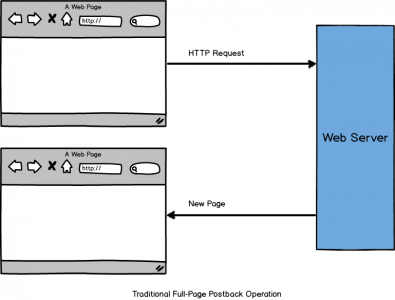
\includegraphics[scale=0.4]{bilder/spi_history_1.png} & & 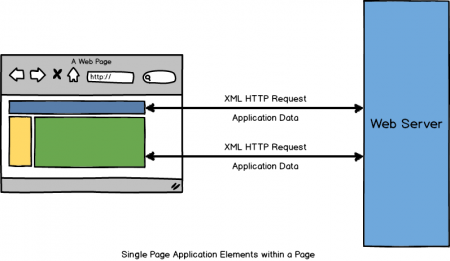
\includegraphics[scale=0.4]{bilder/spi_history_2.png} \\
%			\multicolumn{3}{c}{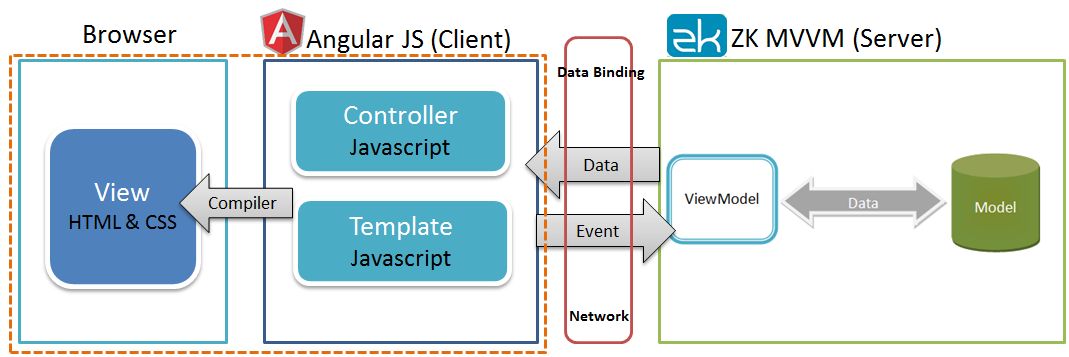
\includegraphics[scale=0.4]{bilder/zk-ng-architecture.png}}
%		\end{tabulary}
%	\end{table}
  \begin{figure}[H]
      \centering
	  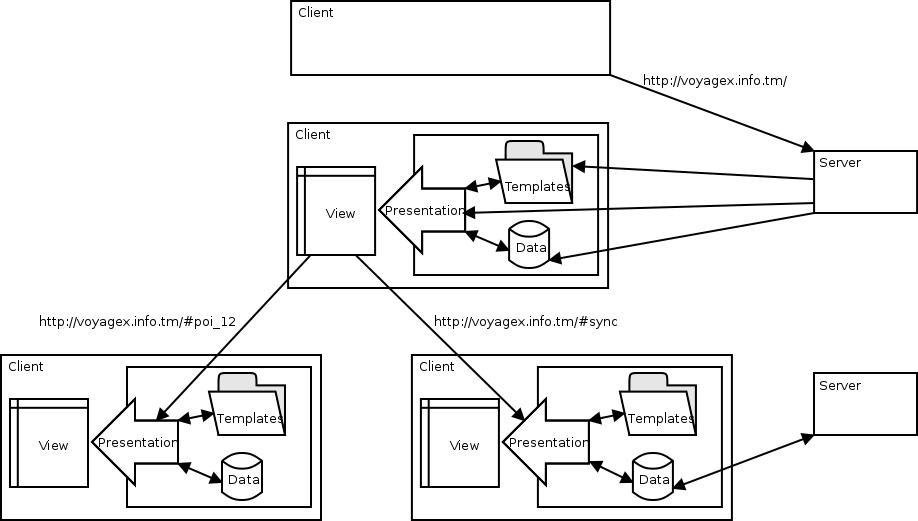
\includegraphics[scale=0.48]{bilder/spi.png}\\ 
  	  \caption{Viewmodel und SPI}
  \end{figure}


%%%%%%%%%%%%%%%%%%%%%%%%%%%%%%%%%%%%%%%%%%%%%%%%%%%%%%%%%%%%%%
% System-Architektur
%%%%%%%%%%%%%%%%%%%%%%%%%%%%%%%%%%%%%%%%%%%%%%%%%%%%%%%%%%%%%%
\subsection{System-Architektur}\label{5_SA}
Die System-Architektur von VoyageX basiert auf dem Client-Server-Modell. Die Darstellungs-Schicht wird am Client implementiert, während die Persistenz-Schicht und die Kommunikations-Schicht auf Client und Server verteilt werden.\\ \\
Die Verteilung der Persistenz-Schicht ist durch die geforderte Offline-Funktionalität bedingt, sie wird über Replikation und Synchronisation eines Ausschnitts der Systemdaten organisiert. In den Abschnitten \ref{DBMS} und \ref{5_DSE} werden die Persistenz-Modelle von Server und Client ausführlicher beschrieben, als Datenaustausch-Format wird JSON genutzt. Die Aufgaben einer serverseitigen Daten-API werden von einer Webanwendung übernommen welche in dieser Hinsicht eher mit der API eines WebServices verglichen werden kann.
Eine weitere Aufgabe der Webanwendung ist die Benutzer-Authentisierung.\\ \\
Die Verteilung der Kommunikationsschicht ist unbedingt, für VoyageX wird sie mit der Publish-Subscribe-Lösung von Faye implementiert. Die Client-Server Komponenten von Faye werden sowohl im Frontend als auch im Backend hinter VoyageX-fähigen Schnittstellen gekapselt, so daß ein späterer Austausch der Kommunikations-Schicht möglich wird, ohne dafür weitere Anwendungs-Teile ändern zu müssen. Die einzelnen Module werden in \ref{5_MESSGNG} vorgestellt.\\
  \begin{figure}[H]
      \centering
	  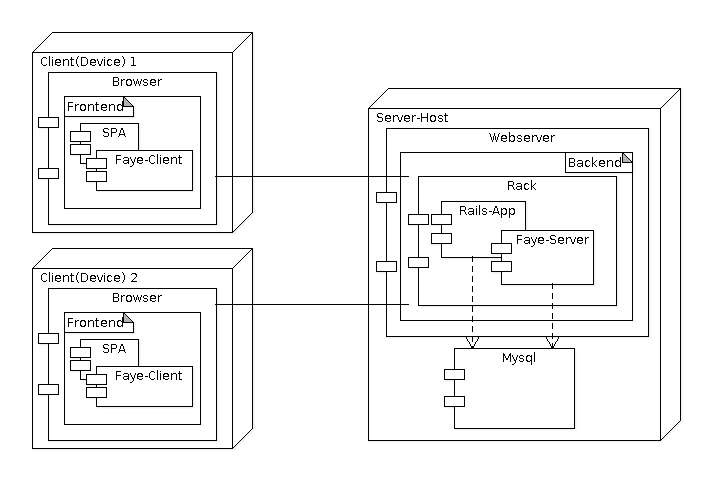
\includegraphics[scale=0.5]{bilder/system_architecture.png}
  	  \caption{Verteilung der System-Komponenten}
  \end{figure}


%%%%%%%%%%%%%%%%%%%%%%%%%%%%%%%%%%%%%%%%%%%%%%%%%%%%%%%%%%%%%%
% Backend
%%%%%%%%%%%%%%%%%%%%%%%%%%%%%%%%%%%%%%%%%%%%%%%%%%%%%%%%%%%%%%
\subsection{Backend}\label{5_BE}
Der Backend-Server erfüllt folgende Aufgaben:
	\begin{itemize}
		\item Bereitstellung der Installations-Konfiguration für die Anwendungs-Initialisierung
		\item Benutzerverwaltung des Systems
		\item Synchronisation der System-Daten für alle Benutzer
		\item Bereitstellung der Kommunikations-Infrastruktur
	\end{itemize}

\subsubsection{Ruby-On-Rails}
Alle Backend-Dienste werden über eine Ruby-On-Rails$^{\textbf{\ref{COMMENT_ROR_1}}}$ (RoR) Web-Anwendung addressiert.%
% footnotes
\addtocounter{footnote}{1}
\footnotetext{\label{COMMENT_ROR_1}Ruby-On-Rails ist ein in der Programmiersprache Ruby geschriebenes Open-Source-Web-Framework mit dem unter anderem durch das "Convention over Configuration" Prinzip eine hohe Produktivität durch schnelle Anwendungs-Entwicklung (Rapid-Application-Development - RAR) erreicht werden kann. \cite{ROR:GETSTA}}%
Wie für alle verbreiteten Programmiersprachen gibt es für Ruby auch zahlreiche Hilfs-Bibiotheken, in der Ruby-Welt Gems genannt, deren modularisierte Funktionalität mit geringem Aufwand in eine RoR-App integriert werden kann $^{\textbf{\ref{GEMINFO1}}}$.
% footnotes
\addtocounter{footnote}{1}%
\footnotetext{\label{GEMINFO1}Viele Gems sind Open-Source-lizensiert}%

\paragraph{Rack}
Rack definiert eine minimale API um Webserver mit Web-Frameworks zu verbinden.\cite{RACK:INTRO}
Diese API besteht aus einer einzigen Methode \texttt{call}, welche mit dem Aufruf-Parameter \texttt{env} ein Http-Request-Objekt sowie Laufzeit-Umgebungs-Informationen an eine Rack-Anwendung übergibt, und als Rückgabe eine Http-Response erwartet, welche dann an den Client zurückgesendet wird.\\
Um RoR-Anwendungen in verschiedene Webserver wie nginx$^{\textbf{\ref{NGINXIDX}}}$%
\addtocounter{footnote}{1}%
\footnotetext{\label{NGINXIDX}\href{http://nginx.org/}{http://nginx.org/}; letzter Zugriff: 22.01.2015}
oder Apache$^{\textbf{\ref{APACHEIDX}}}$%
\addtocounter{footnote}{1}%
\footnotetext{\label{APACHEIDX}\href{http://httpd.apache.org/}{http://httpd.apache.org/}; letzter Zugriff: 22.01.2015}
zu integrieren, können Rack-Server von diesen als Plugin eingebunden werden. Die Integration anwendungsspezifischer Netzwerk-Funktionalität wird durch eine modularisierte Middleware-Schicht ermöglicht. So wird beispielsweise in VoyageX die Kommunikations-Schicht durch die Faye-Middleware implementiert, welche den Webserver um eigene, für die RoR-Anwendung völlig transparente, Protokolle erweitert.\\
% Rails-Anwendungen sind Rack-Anwendungen

\paragraph{Gems}\noindent
Die in einer RoR-App eingebundenen Hilfsbibliotheken können nach verschiedenen Kritierien kategorisiert werden.
	\begin{itemize}
		\item Laufzeit-Umgebung
		\item Infrastruktur
		\item Anwendungslogik
	\end{itemize}
In Ruby-Anwendungen, also auch in Rails-Webanwendungen, werden häufig Module oder Bibliotheken mittels RubyGems eingebunden, um bereits verfügbare Lösungen nicht selbst programmieren zu müssen$^{\textbf{\ref{CMT_GEM}}}$%
\addtocounter{footnote}{1}%
\footnotetext{\label{CMT_GEM}Nicht alle Gems werden als OpenSource angeboten}
. Viele allgemeine Gems einer Rails-App werden quasi standardmäßig genutzt, dazu zählen Syntactic-Sugar Gems wie Haml$^{\textbf{\ref{HAMLIDX}}}$%
\addtocounter{footnote}{1}%
\footnotetext{\label{HAMLIDX}\href{http://haml.info/}{http://haml.info/}; letzter Zugriff: 22.01.2015}
und Sass$^{\textbf{\ref{SASSIDX}}}$%
\addtocounter{footnote}{1}%
\footnotetext{\label{SASSIDX}\href{http://sass-lang.com/}{http://sass-lang.com/}; letzter Zugriff: 22.01.2015}
, oder aber Code-Bibliotheken wie jQuery$^{\textbf{\ref{JQUERYIDX}}}$%
\addtocounter{footnote}{1}%
\footnotetext{\label{JQUERYIDX}\href{https://jquery.com/}{https://jquery.com/}; letzter Zugriff: 22.01.2015}.\\
Anwendungs-spezifische für VoyageX Gems sind:\\
\lstset{language=CoffeeScript}
\begin{lstlisting}[frame=single,xleftmargin=0pt,numbers=none]
  gem "devise"
  gem "omniauth-facebook"
  gem "geocoder"
  gem "paperclip", "~> 4.2"
  group :production, :staging, :development do
    gem "comm", path: "comm-plugin"
  end
  gem "resque-scheduler" 
\end{lstlisting}
\subparagraph{devise:}Ein Autorisierungs-Paket, das konfigurierbare Implementierungen von Registrierungs-Logik mit optional erforderlicher Email-Bestätigung, über Session-Verwaltung, bis hin zur Authentisierung durch Dritte, also beispielsweise Social Networks wie Facebook und Twitter, oder aber auch LDAP enthält.\\
Verschiedene Strategien werden als Plugins in Devise integriert. In der Anwendung sind dann Utility-Methoden
verfügbar, wie besipielsweise:
\lstset{language=Ruby}
\begin{lstlisting}[frame=single,xleftmargin=0pt,numbers=none]
  current_user
  signed_in?
\end{lstlisting}
\subparagraph{omniauth-facebook:}Die Implementierun einer Devise-Strategie für die Authentisierung über ein Facebook-Account. Im View-Code muss nur noch, wie im folgenden Haml-Snippet, ein Link eingebettet werden, den Rest erledigt das Gem:
\begin{lstlisting}[frame=single,xleftmargin=0pt,numbers=none]
.button.facebook_login
  = link_to image_tag("fb-icon.png"), user_omniauth_authorize_path(:facebook)
\end{lstlisting}
\subparagraph{paperclip:}Paperclip bietet Funktionen zur Integration hochgeladener Dateien in Active-Record. Die Dateien können auch über Konfigurations-Parameter automatisiert vor- und nach-bearbeitet werden, beispielsweise können Bilder skaliert und/oder in verschiedene Formate konvertiert werden.
\begin{lstlisting}[frame=single,xleftmargin=0pt,numbers=none]
  current_user.avatar(:medium_size)
\end{lstlisting}
\subparagraph{resque:}ist eine Redis-Db-gestützte Bibliothek zur Ausführung asynchroner Jobs. Komplexe bzw. aufwendige Operationen sollten nicht im Request-Response Zyklus der Webanwendung ausgeführt werden da sonst
der Server blockiern könnte. In VoyageX wird Resque bei der Synchronisation der Benutzer-Daten-Kopie mit der Master-Kopie eingesetzt. Das Kommunikations-Modul von Faye nutzt Resque ebenfalls.
\subparagraph{comm:}comm ist eine für VoyageX entwickelte Rails-Plugin-Anwendung, welche die Kommunikations-Komponente von der eigentlichen VoyageX-Webapp trennt, in dem sie in einem eigenen Engine$^{\textbf{\ref{RAILSENG}}}$%
\addtocounter{footnote}{1}%
\footnotetext{\label{RAILSENG}\href{http://api.rubyonrails.org/classes/Rails/Engine.html}{Rails-Engine http://api.rubyonrails.org/classes/Rails/Engine.html}; letzter Zugriff: 22.01.2015}
(mit eigenem Middleware-Stack) in Rack läuft - zur Laufzeit hat das Plugin aber Zugriff auf alle Resourcen der Anwendung. Durch diese Trennung kann VoyageX jederzeit auf ein anderes Kommuniations-System umgestellt, und der Faye-spezifische Teil ersetzt werden.\\
Neben der weiter oben gezeigten Deklaration im Gem-File muss das Plugin noch mittels Eintrag in der Konfigurations-Datei "`config/routes.conf"' in die Anwendung integriert werden, damit alle Requests, die mit einem festzulegenden Url-Pfad-Prefix (hier "`/comm"') beginnen, vom Rack-Server zur Abarbeitung an das Plugin weitergereicht werden.
\begin{lstlisting}[frame=single,xleftmargin=0pt,numbers=none]
  mount FayeComm::Engine => "/comm"
\end{lstlisting}
In der Datei "`comm-plugin/lib/faye\_comm/engine.rb"' wird die Plugin-eigene Middleware konfiguriert. 
\lstset{language=CoffeeScript}
\begin{lstlisting}[frame=single,xleftmargin=0pt,numbers=none]
module FayeComm
  class Engine < ::Rails::Engine
    config.middleware.use FayeRails::Middleware, { mount: '/', timeout: 25 }.merge!(engine_params) do
      map '/**' => FayeComm::ChannelsController
    end
  end
end
\end{lstlisting}
Die dafür erforderlichen Gems werden in "`comm-plugin/comm.gemspec"' eingetragen.
\lstset{language=CoffeeScript}
\begin{lstlisting}[frame=single,xleftmargin=0pt,numbers=none]
  s.add_dependency "faye-rails", "2.0.0"
\end{lstlisting}

\subparagraph{faye-rails:}\label{FAYERAILS}Faye-Rails ist die vom FayeComm-Plugin eingebundene Rack-Middleware, welche
die Server-Komponente eines Public-Messaging-Systems implementiert. Faye bietet ihrerseits widerum eine Schnittstelle zur Integration anwendungs-spezifischer Funktionen in die Kommunikations-Abläufe. Dafür wird von VoyageX der in \ref{CTRLS_CHANNEL} beschriebene Controller entwickelt.
 
\paragraph{Controllers}\noindent
Rails unterstützt das Routing nach dem Representational State Transfer (Rest) Paradigma. Dieses zielt darauf ab, die Eindeutigkeit von Urls bezüglich der damit referenzierten Resourcen zu standardisieren, um ähnlich wie bei Web-Services auch ohne Kenntnis der Implementierung eines Dienstes bestimmte Standard-Operationen wie z.b. Create, Read, Update und Delete (CRUD) auf Resourcen durchführen zu können. Zusätzlich werden durch die Request-Parameter auch die Daten-Repräsentations/Ausgabe-Formate der Resource beim Aufruf durch den Accept-Header festgelegt.\\
Jede Url wird in Rails auf einen Methode (Action) eines Controllers verlinkt (gemapped). Diese Zuordnung
wird in der datei "`config/routes.rb"' festgelegt.\\
Folgender Eintrag erzeugt beispielsweise ein Mapping für put-Requests auf die url /sync\_poi/:id, wobei :id ein Platzhalter für eine beliebige Zeichenfolge sein kann - im vorliegenden Fall wird damit eine Poi-Id gekennzeichnet. Der Request wird von Rails dann an die Methode "`sync\_poi"' der Klasse "`PoisController"' übergeben.\\
\begin{lstlisting}[frame=single,xleftmargin=0pt,numbers=none,caption={Konfiguration einer Url in conf/routes.rb},captionpos=b]
  put '/sync_poi/:id', to: 'pois#sync_poi', as: :sync_poi
\end{lstlisting}

\subparagraph{MainController:}
Die Anwendung wird mit dem Aufruf der Root-Url (http://voyagex.info.tm/) gestartet, welcher
zur Methode "`index"' der Klasse "`MainController"' gemapped und dort abgearbeitet wird. 
\begin{itemize}[leftmargin=*,noitemsep,topsep=1ex,parsep=0pt,partopsep=0pt]
\item \textbf{index}: beim Start der Anwendung wird zuerst eine Benutzer-Umgebung initialisert:
  \begin{itemize}[leftmargin=*,noitemsep,topsep=1ex,parsep=0pt,partopsep=0pt]
    \item Publish/Subscribe Kommunikationskanäle werden für den Benutzer konfiguriert (CommPort).
    \item für registrierte Benutzer werden Synchronisations-Management-Parameter aktualisiert (Daten-Replikations-Repository).
  \end{itemize}
Mit weiteren Benutzer-Umgebungs-Variablen wird anschliessend das Viewmodel initialisert, und zusammen mit den Rohdaten und den Templates an den Client gesendet. Im Browser wird dann eine  initiale Kartenansicht mit allen POIs und Kontakten im aktuellen geographischen Ausschnitt angezeigt.
\item \textbf{manifest}: Beim Aufruf dieser Methode wird das Application-Cache-Manifest-File generiert. Insbesondere werden dem Benutzer dabei Versionsänderungen von Asset-Files, also Javascript-, CSS- und Media-Dateien, angezeigt. (siehe auch \ref{5_OFFL})
\end{itemize}
\subparagraph{PoisController:}
\begin{itemize}[leftmargin=*,noitemsep,topsep=1ex,parsep=0pt,partopsep=0pt]
\item \textbf{sync\_poi}: Diese Action wird aufgerufen wenn ein Benutzer Änderungen der POI-Einträge durchgeführt hat, also neue POIs eingetragen oder bestehende POIs kommentiert hat.\\
Jede Änderung der Systemdaten wird mit einer Commit-Hash-ID gekennzeichnet. Nach dem sichern der Daten erhalten alle Clients der anderen Benutzer über die Kommunikations-Schicht eine Nachricht mit Standort- und Verfasser-Informationen. Bei allen Clients, deren angezeigter Kartenabschnitt die Position des geänderten POIs beinhaltet, oder die mit dem Verfasser in einer Kontakt-Beziehung stehen, werden die lokalen Daten aktualisiert und die Benutzer mit einem visuellen und/oder akkustischen Signal benachrichtigt.
\item \textbf{pois}: API-Methode: liefert alle POIs im Umkreis einer durch "`Latitude"' und "`Longitude"' bestimmten Position.
\item \textbf{comments}: API-Methode: liefert alle Kommentare zu einem POI.
\end{itemize}
%Die letzten beiden Methoden werden von der APP aufgerufen wenn synchronisiert wird ohne daß der clienet selbst was geändert hat.
\subparagraph{UsersController:}
\begin{itemize}[leftmargin=*,noitemsep,topsep=1ex,parsep=0pt,partopsep=0pt]
\item \textbf{update\_peers}: In dieser Methode werden die Kontakte, also die Follow-Beziehungen zu anderen Benutzern festgelegt.
  \begin{itemize}[leftmargin=*,noitemsep,topsep=1ex,parsep=0pt,partopsep=0pt]
    \item Follow-Anfrage an entfernten Benutzer stellen (request)
    \item Follow-Anfrage eines entfernten Benutzer annehmen oder ablehnen (grant / deny)
    \item Eine vom lokalen Benutzer erteilte Follow-Erlaubnis entziehen (revoke)
    \item Auf eine Follow-Erlaubnis von einem entfernten Benutzer verzichten (cancel)
  \end{itemize}
\end{itemize}
\subparagraph{Auth::RegistrationsController:}
\begin{itemize}[leftmargin=*,noitemsep,topsep=1ex,parsep=0pt,partopsep=0pt]
\item \textbf{create}: In dieser Methode wird ein neuer Benutzer registriert: Die Zugangsdaten werden gesichert und die Email-Adresse wird durch eine Bestätigungs-Email$^{\textbf{\ref{COMMENT_CONF_MAIL}}}$%
\addtocounter{footnote}{1}%
\footnotetext{\label{COMMENT_CONF_MAIL}In einer Bestätigungsmail ist eine Url mit einem Zeichenschlüssel angegeben, die der Benutzer aufrufen muß um den Erhalt der Email zu bestätigen.}
verifizert.
\end{itemize}
\subparagraph{Auth::SessionsController:}
\begin{itemize}[leftmargin=*,noitemsep,topsep=1ex,parsep=0pt,partopsep=0pt]
\item \textbf{create}: Diese Methode initialisert eine neue Session für den mit Email-Adresse und Passwort authentifizierten Benutzer 
\item \textbf{destroy}: Diese Methode beendet eine Session, so daß kein anderer Nutzer des Browsers die Anwendung mit der Authentität des Benutzers weiter nutzen kann.
\end{itemize}
\subparagraph{Auth::OmniauthCallbacksController:}
\begin{itemize}[leftmargin=*,noitemsep,topsep=1ex,parsep=0pt,partopsep=0pt]
\item \textbf{self.provides\_callback\_for}: Diese Methode wird von dritten Authentisierungs-Authoritäten aufgerufen. (z.B. Facebook, Twitter, LDAP, ...)
\end{itemize}
\subparagraph{Comm::CommController:}
\begin{itemize}[leftmargin=*,noitemsep,topsep=1ex,parsep=0pt,partopsep=0pt]
\item \textbf{register}: Diese Methode wird aufgerufen, wenn sich ein Client neu mit der Kommunikations-Schicht verbindet.
Die Clients aller Kontakte des Benutzers werden über dieses Ereignis informiert und können dann die Kommunikationskanäle des Benutzers abonnieren.
\end{itemize}
\subparagraph{Comm::ChannelsController:}\label{CTRLS_CHANNEL}
Der ChannelsController wird von FayeRails::Controller abgeleitet und ermöglicht eine Integration eigener Kommunikations-Steuerungungs-Logik.\\
\lstset{language=CoffeeScript}
\begin{lstlisting}[frame=single,xleftmargin=0pt,numbers=none]
channel '/talk**' do
  monitor :subscribe do
    Rails.logger.debug "###### Client #{client_id} subscribed to #{channel}."
  end
  monitor :unsubscribe do
    Rails.logger.debug "###### Client #{client_id} unsubscribed from #{channel}."
  end
  monitor :publish do
    Rails.logger.debug "###### Client #{client_id} published #{data.inspect} to #{channel}."
  end
end
\end{lstlisting}
In VoyageX wird diese Möglichkeit genutzt, um:
\begin{itemize}[leftmargin=*,noitemsep,topsep=1ex,parsep=0pt,partopsep=0pt]
\item unauthorisierte Kanal-Zugriffe zu blockieren
\item Nachrichten mit Reverse-Geocoding-Daten anzureichern.
\end{itemize}

\subsubsection{Datenbank-Management-System (DBMS)}
Die VoyageX-RoR-Anwendung nutzt für die Implementierung des Daten-Modells (Model) das Object-Relational-Mapping$^{\textbf{\ref{CMTORM}}}$%
% footnote
\addtocounter{footnote}{1}%
\footnotetext{\label{CMTORM}Beim ORM werden Tabellen einer relationalen Datenbank über Objekte referenziert.}
(ORM) Gem ActiveRecord$^{\textbf{\ref{CMTAR}}}$%
\addtocounter{footnote}{1}%
\footnotetext{\label{CMTAR}\href{http://api.rubyonrails.org/classes/ActiveRecord/Base.html}{Active Record http://api.rubyonrails.org/classes/ActiveRecord/Base.html}; letzter Zugriff: 22.01.2015}
, das für die Speicherung der System-Daten eine konfigurierbare Auswahl verschiedener Anbieter von relationalen DBMS erlaubt. Für VoyageX wurde MySQL$^{\textbf{\ref{CMTMYSQL}}}$%
\addtocounter{footnote}{1}%
\footnotetext{\label{CMTMYSQL}\href{http://de.wikipedia.org/wiki/MySQL}{MySQL - http://de.wikipedia.org/wiki/MySQL}; letzter Zugriff: 22.01.2015} gewählt.\\ \\
In einem relationalen Entwurf werden die von der Anwendung verwendeten Komponenten in einem Schema definiert.
\paragraph{ER-Schema}
Für die Abbildung der Daten werden folgende Entitäten eingeführt. \\

  \begin{figure}[H]
      \centering
	  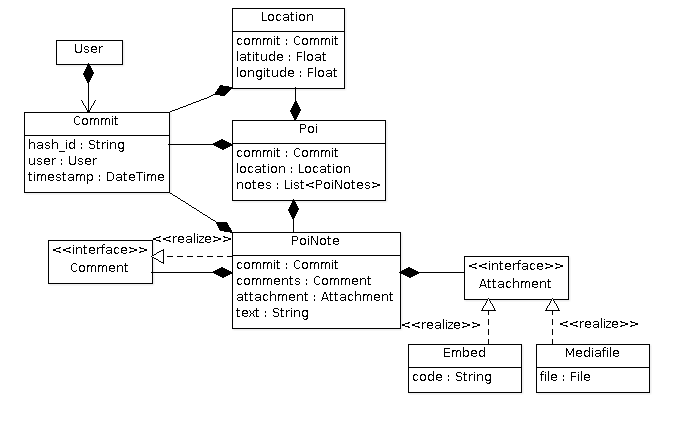
\includegraphics[scale=0.6]{bilder/uml/er_poi.png}
  	  \caption{POI-Schema}
  \end{figure}

\begin{itemize}[leftmargin=*,noitemsep,topsep=1ex,parsep=0pt,partopsep=0pt]
\item \textbf{Location}: Jeder Markierung auf der Karte ist ein Eintrag in der Tabelle "`locations"' zugeordnet. Alle Entitäten sind direkt oder indirekt mit einem Ort verbunden.
\item \textbf{Poi}: Ein Poi besteht aus der Location und mindestens einer POI-Note.
\item \textbf{PoiNote}: Poi-Beschreibung -Kommentar Textform, optional mit einem Multimedia-Anhang.
\item \textbf{Embed, Mediafile}: Attachment-Content-Typen.
\item \textbf{Commit}: Jede Änderung der System-Daten und der daraus resultierende Zusand kann über einen Commit referenziert werden. Ein Commit kann aus einem oder mehreren zu einer einzigen Transaktion zusammengefassten Änderungsschritten bestehen. Commits dienen der Synchronisation von replizierten Benutzer-Kopien mit den System-Masterdaten. 
\end{itemize}

  \begin{figure}[H]
      \centering
	  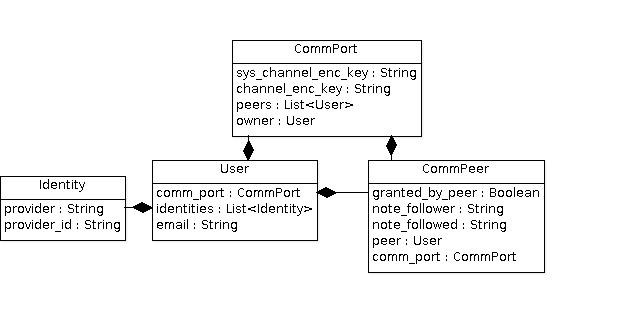
\includegraphics[scale=0.6]{bilder/uml/er_user.png}
  	  \caption{User-Schema}
  \end{figure}

\begin{itemize}[leftmargin=*,noitemsep,topsep=1ex,parsep=0pt,partopsep=0pt]
\item \textbf{User}: Anwendungs-Benutzer
\item \textbf{Identity}: Benutzer können auf verschiedene Weise authentisiert werden, z.B. durch lokale Registrierung mit Passwort und Email oder über eine Dritten wie Soziale Netzwerke. Für einen Benutzer können mehrere Autorisierungs-Anbieter existieren.
\item \textbf{CommPort}: Die Kommunikations-Schnittstelle eines Benutzer.
\item \textbf{CommPeer}: Die Abbildung einer P2P-Beziehung. Benutzer folgen dem CommPort eines anderen Benutzers. Im Feld \texttt{granted\_by\_peer} wird der Autorisierungs-Status der Beziehung gesetzt. Zusätzlich können beide Benutzer Notizen zu der Beziehung speichern.
\end{itemize}


\subsubsection{Messaging}\label{5_MESSGNG}
Als Implementierung einer synchronen Kommunikation zwischen online-Benutzern wurde für VoyageX die Publish-Subscribe-Messaging-Lösung \texttt{Faye} gewählt, deren Client-Implementierung von allen aktuell verbreiteten Browsern unterstützt wird.\\
An dieser Stelle soll aber von den alternativen Möglicheiten wenigstens WebRTC angeführt werden, da es sich dabei um einen im Draft-Status befindlichen W3C-Standard handelt.
% Zur Zeit befindet sich aber ein Standard in Entwicklung, der im Falle der Verfügbarkeit in allen Browsern bzw. auf allen Plattformen die erste Wahl wäre, so daß er hier kurz vorgestellt werden soll. Die Kommunikations-Schicht ist bei VoyageX aber soweit geschichtet, so daß ein Wechsel ohne Anpassungen der restlichen Anwendungsfunktionen möglich ist. \\
%In der Rack-Anwendung des Backends wird die Kommunikations-Schnittstelle mittels Gem als Rails-Plugin in einem eigenen Engin gemounted

\paragraph{Web-Real-Time-Communication - WebRTC$^{\textbf{\ref{CMTMYSQL}}}$}
\addtocounter{footnote}{1}%
\footnotetext{\label{CMTMYSQL}\href{http://de.wikipedia.org/wiki/WebRTC}{WebRTC - http://de.wikipedia.org/wiki/WebRTC}; letzter Zugriff: 22.01.2015}
WebRTC ist eine auf Html5 basierende Schnittstellen-Definition, die eine Audio- und Video-Übertragung auf Peer-To-Peer Basis realisiert. Diese API teilt sich in die Bereiche:
\begin{itemize}[leftmargin=*,noitemsep,topsep=1ex,parsep=0pt,partopsep=0pt]
\item Protokolle und Mechanismen zum Aufbau einer Kommunikations-Infrastruktur
\item Zugriff auf die in der plattform-spezifischen Laufzeit-Umgebung verfügbaren Multimedia-Hardware-Komponenten
\end{itemize}
Derzeit wird der Standard aber noch nicht von Safari (IOS/MacOS) oder IE unterstützt - für eine plattformübergreifende Kommunikations-Lösung ist WebRTC also noch nicht geeignet.\\
In VoyageX wird allerdings die Hardware-Zugriffs-API der WebRTC für die Aufnahme von Fotos unter Chrome und Firefox verwendet, für andere Browser werden dafür andere, plattform-spezifische Lösungen bereitgestellt.
%es gibt zwar auch einen ansatz atlassian als plugin zu 

\paragraph{Faye}
Die Plattformunabhängigkeit wird im Faye-Client vor allem durch die Implementierung mehrerer Transport-Protokoll-Alternativen erreicht. Je nach Plattform und Technologie-Verfügbareit wählt der Client aus folgenden Kommunikations-Protokollen/Strategien:
	\begin{itemize}
		\item Persistente Verbindungen mit WebSockets
		\item Long-polling via HTTP POST
		\item Cross Origin Resource Sharing
		\item Callback-polling via JSON-P
	\end{itemize}
%TODO: Akku-Verbrauch bei mobilen Clients analysieren
Für die Faye-Lösung spricht aber auch die bereits vollständig implementierte Messaging-Kommunikations-Infrastruktur und die damit verbundene Verminderung des eigenen Programmier-Aufwandes.\\
Die Kommunikation über Faye basiert auf dem \texttt{Bayeux}-Protokoll$^{\textbf{\ref{CMTBAYX}}}$%
\addtocounter{footnote}{1}%
\footnotetext{\label{CMTBAYX}\href{http://svn.cometd.org/trunk/bayeux/bayeux.html}{Bayeux - http://svn.cometd.org/trunk/bayeux/bayeux.html}; letzter Zugriff: 22.01.2015} und einer Server-Client-Architektur, wobei alle
Komponenten frei verfügbar sind.
Implementierungen des Faye-Servers gibt es für \texttt{Rack}- und \texttt{Node.js}.
Die Server-Komponente wird bei Rack, wie in \ref{FAYERAILS} beschrieben, als Middleware in das Backend integriert.\\
Die Client-Komponente bietet ebenso eine einfache Kommunikations-Schnittstelle mit den Methoden:
\begin{itemize}[leftmargin=*,noitemsep,topsep=1ex,parsep=0pt,partopsep=0pt]
\item publish
\item subscribe
\end{itemize}


%%%%%%%%%%%%%%%%%%%%%%%%%%%%%%%%%%%%%%%%%%%%%%%%%%%%%%%%%%%%%%
% Frontend
%%%%%%%%%%%%%%%%%%%%%%%%%%%%%%%%%%%%%%%%%%%%%%%%%%%%%%%%%%%%%%
\subsection{Frontend}\label{5_FE}
Wenn eine Single-Page-Interface Webanwendung mit dem Model-View-Controller (MVC) Muster realisiert wird, dann werden die MVC-Komponenten \texttt{View} und \texttt{Controller} im Client implementiert. Die \texttt{Model}-Komponenten befinden sich am Backend-Server, wobei die Daten dann mittels Databinding$^{\textbf{\ref{CMTDATABIN}}}$ gelesen und gesichert werden. Nach Daten-Änderungen wird dann die aktualisierte Ansicht der GUI mit Javascript aus Html-Templates, CSS und den Daten neu generiert. Bei einer offline-fähigen Anwendung wie VoyageX werden auch die Model-Komponenten im Client implementiert, da der Client eine eigene, von einer Netzwerk-Verbindung unabhängige Persistenz-Verwaltung benötigt.

\subsubsection{Anforderungen an den Client / Browser}\label{4_ACB}
%VoyageX soll als Single Page (Web-)Application (SPA) realisiert und kann 
VoyageX soll zwar mit verschiedenen Browsern auf unterschiedlichen Plattformen / Betriebssystemen genutzt werden können, bei der angestrebten Plattformunabhängigkeit gibt es aber dennoch Einschränkungen. Die volle Funktionalität kann auf mobilen Endgeräten nur für den Chrome-Browser unter Android, und auf Desktop-Rechnern für den Chrome-Browser unter Linux garantiert werden.

\paragraph{Html5}
Html5$^{\textbf{\ref{HTML5}}}$%
% footnote
\addtocounter{footnote}{1}%
\footnotetext{\label{HTML5}\href{http://www.w3.org/blog/news/archives/4167}{Html5 - http://www.w3.org/blog/news/archives/4167}; letzter Zugriff: 01.03.2015}
ist die fünfte Version des Html Standards. Im Vergleich zu Html4 wurde auch die Multimedia-Schnittstelle wesentlich erweitert, um auch die Nutzung neuer Hardware-Technologien aus diesem Bereich in einer Web-Anwendung anbieten zu können. VoyageX setzt HTML5-fähige Browser-Versionen voraus. 
  \begin{figure}[H]
  \begin{adjustwidth}{-1.5cm}{1.5cm}
      \centering
	  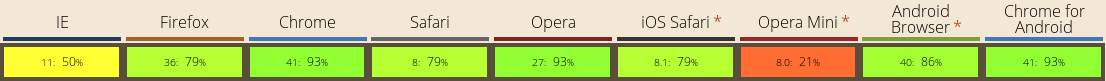
\includegraphics[scale=0.6]{bilder/screenshots/caniuse_html5.png}\\ 
  	  \caption{Noch nicht alle Features von Html5 werden von allen Browsern unterstützt.
  	  Quelle: caniuse$^{\textbf{\ref{CIU_HTML5}}}$}
  \end{adjustwidth}
  \end{figure}
% footnote
\addtocounter{footnote}{1}%
\footnotetext{\label{CIU_HTML5}\href{http://caniuse.com/\#search=html5}{http://caniuse.com/\#search=html5}; letzter Zugriff: 01.03.2015}

\paragraph{Web Storage}
Web Storage war ursprünglich Teil der Html5 Spezifikation, ist aber mittlerweile ein eigener Standard$^{\textbf{\ref{WEBSTRG}}}$%
% footnote
\addtocounter{footnote}{1}%
\footnotetext{\label{WEBSTRG}\href{http://www.w3.org/TR/webstorage/}{Web Storage - http://www.w3.org/TR/webstorage/}; letzter Zugriff: 01.03.2015}
. Von den beiden Teil-Komponenten Session Storage und Local Storage nutzt VoyageX letztere zum Speichern von Anwendungsdaten für den Offline-Betrieb.
  \begin{figure}[H]
  \begin{adjustwidth}{-1.5cm}{1.5cm}
      \centering
	  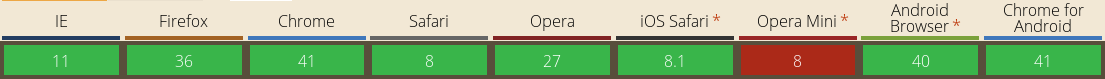
\includegraphics[scale=0.6]{bilder/screenshots/caniuse_webstorage.png}\\ 
  	  \caption{Quelle: caniuse$^{\textbf{\ref{CIU_WEBST}}}$}
  \end{adjustwidth}
  \end{figure}
% footnote
\addtocounter{footnote}{1}%
\footnotetext{\label{CIU_WEBST}\href{http://caniuse.com/\#search=webstorage}{http://caniuse.com/\#search=webstorage}; letzter Zugriff: 01.03.2015}

\paragraph{Application Cache}
Im Application Cache kann die Anwendung Quelldateien, wie Javascript und CSS-Stylesheets, Bild-Dateien oder andere statischen Anwendungskomponenten für einen späteren Gebrauch im Offline-Modus vom Browser speichern lassen. Die zu speichernden Komponenten werden dabei in einer Manifest-Datei$^{\textbf{\ref{CACMAN}}}$%
% footnote
\addtocounter{footnote}{1}%
\footnotetext{\label{CACMAN}\href{http://en.wikipedia.org/wiki/Cache_manifest_in_HTML5}{Cache Manifest - http://en.wikipedia.org/wiki/Cache\_manifest\_in\_HTML5}; letzter Zugriff: 01.03.2015}
notiert. 
  \begin{figure}[H]
  \begin{adjustwidth}{-1.5cm}{1.5cm}
      \centering
	  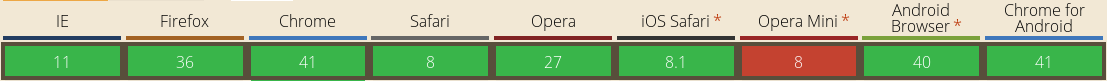
\includegraphics[scale=0.6]{bilder/screenshots/caniuse_appcache.png}\\ 
  	  \caption{Quelle: caniuse$^{\textbf{\ref{CIU_APPC}}}$}
  \end{adjustwidth}
  \end{figure}
% footnote
\addtocounter{footnote}{1}%
\footnotetext{\label{CIU_APPC}\href{http://caniuse.com/\#search=Application\%20Cache}{http://caniuse.com/\#search=Application\%20Cache}; letzter Zugriff: 01.03.2015}

\paragraph{File API}
Die File-API ist eine von Html5 definierte Javascript-Schnittstelle die es einer Anwendung erlaubt, Dateien lokal zu speichern. Im Gegensatz zum \texttt{localStorage}, welches nur das Speichern von Zeichenketten ermöglicht, hat man hier ein echtes Filesystem zur Verfügung. Ein entscheidender Vorteil gegenüber dem localStorage ist es, daß die maximale Speicherkapazität nach oben nicht durch 5 MB beschränkt ist, sondern vom Benutzer festgelegt wird. Daten können somit auch im Gigabyte-Bereich im Client abgelegt werden.
  \begin{figure}[H]
  \begin{adjustwidth}{-1.5cm}{1.5cm}
      \centering
          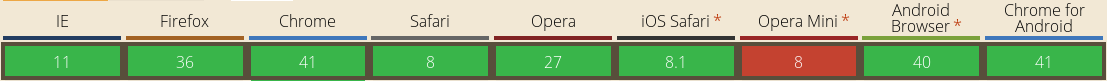
\includegraphics[scale=0.6]{bilder/screenshots/caniuse_fileapi.png}\\ 
          \caption{Quelle: caniuse$^{\textbf{\ref{CIU_FILEAPI}}}$}
  \end{adjustwidth}
  \end{figure}
% footnote
\addtocounter{footnote}{1}%
\footnotetext{\label{CIU_FILEAPI}\href{http://caniuse.com/\#search=file\%20api}{http://caniuse.com/\#search=file\%20api}; letzter Zugriff: 01.03.2015}

\paragraph{Media Providers}
Mit \texttt{MediaSource} und \texttt{MediaStream} sind in Html5 Javascript-Schnittstellen definiert, die das Aufnehmen und Abspielen von Audio bzw. Videodateien ermöglichen. Insbesondere können auch Fotos in Form von Video-Snapshots aufgenommen werden.
  \begin{figure}[H]
  \begin{adjustwidth}{-1.5cm}{1.5cm}
      \centering
          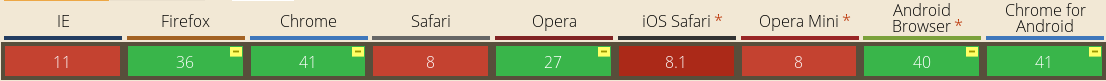
\includegraphics[scale=0.6]{bilder/screenshots/caniuse_mediastream.png}\\ 
          \caption{Quelle: caniuse$^{\textbf{\ref{CIU_MEDIASTR}}}$}
  \end{adjustwidth}
  \end{figure}
% footnote
\addtocounter{footnote}{1}%
\footnotetext{\label{CIU_MEDIASTR}\href{http://caniuse.com/\#search=Media\%20Stream}{http://caniuse.com/\#search=Media\%20Stream}; letzter Zugriff: 01.03.2015}

\subsubsection{Coffee-Script}
Die Anwendungs-Logik des Frontends von VoyageX ist in \texttt{CoffeeScript}$^{\textbf{\ref{CMTBAYX}}}$%
\addtocounter{footnote}{1}%
\footnotetext{\label{CMTBAYX}\href{http://de.wikipedia.org/wiki/CoffeeScript}{CoffeeScript - http://de.wikipedia.org/wiki/CoffeeScript}; letzter Zugriff: 22.01.2015} geschrieben, welches im Backend vor dem Laden durch den Browser in JavaScript transkompiliert wird.\\
Ein wesentlicher Nutzen von CoffeeScript ist die Verbesserung der Lesbarkeit von Javascript-Code. Dies wird durch eine klare objektorientierte Syntax und durch weitere Syntactic-Sugar-Features und funktionale Utilitiy-Methoden erreicht. Bei zunehmender Anwendungs-Komplexität ist es schwierig, übersichtlichen Programm-Code mit herkömmlichen JavaScript herzustellen, dabei soll CoffeeScript Hilfe leisten. Ein weiterer Vorteil ist die Erkennung von Syntaxfehlern beim Transkompilieren$^{\textbf{\ref{CMTBAYX}}}$%
\addtocounter{footnote}{1}%
\footnotetext{\label{CMTBAYX}Compiler bieten durch statische Code-Analyse generell gute Möglichkeiten zur Fehlererkennung.}. 

\subsubsection{Datenspeicherung und Entitäten}\label{5_DSE}
Eine Nutzung der Anwendung bei fehender Netzwerkverbindung erfordert folgende lokale Daten-Strukturen:
\begin{itemize}[leftmargin=*,noitemsep,topsep=1ex,parsep=0pt,partopsep=0pt]
\item eine Replikation jener Systemdaten, die für den lokalen Benutzer relevant sind. Die Relevanz wird im Falle der POI-Daten durch den vom Benutzer festgelegten Kartenauschnitt entschieden. 
\item Daten über entfernte Benutzer, diese werden über die Kontakt-Beziehung gewichtet.
\item POI-Daten die der Benutzer im Offline-Modus selbst erstellt.
\end{itemize}
Für Speichern und Verwaltung von Daten im Client-Browser gibt es mehrere Möglichkeiten die sich nach Kapazität und Plattform-Verfügbarkeit unterscheiden.

\paragraph{localStorage (Webstorage), IndexedDB, WebSQL und File-API}

	\begin{table}[H]
		\centering
		\begin{tabulary}{\columnwidth}{|L|C|C|C|C|}
		\hline
			& \textbf{Webstorage} & \textbf{IndexedDB$^{\textbf{\ref{CMTIDXDB}}}$%
\addtocounter{footnote}{1}%
\footnotetext{\label{CMTIDXDB}\href{http://de.wikipedia.org/wiki/Indexed\_Database\_API}{IndexedDB - http://de.wikipedia.org/wiki/Indexed\_Database\_API}; letzter Zugriff: 22.01.2015}} & \textbf{WebSQL} & \textbf{File-API} \\ \hline
%						  1   2   3	  4   5   6   7   8   9   10  11  12  13  14  15		
			W3C-Recommendation     & Y & Y & N & N \\ \hline
			Plattform     & IE,FF,CH,SA,OP & FF,CH,OP & CH,SA,OP & IE,FF,CH,SA,OP \\ \hline
			Größen-Limit     & 5-10MB & 10\%HD & - & - \\ \hline
			Storage-Type    & Key-Value & ObjectStore & Relational & Filesystem \\ \hline
		\end{tabulary}
		\caption{Client-seitige Persistenz-APIs}
	\end{table}
Als kommender Standard und wegen der Speicherkapazität und den erweiterten Such- bzw. Abfrage-Funktionen wäre \texttt{IndexedDB} eine gute Wahl, allerdings fehlt dafür noch die Unterstützung auf wichtigen Plattformen. 
  \begin{figure}[H]
  \begin{adjustwidth}{-1.5cm}{1.5cm}
      \centering
	  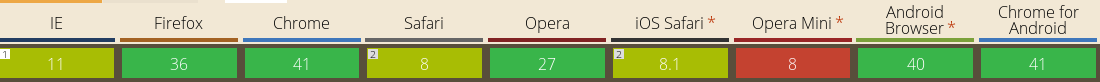
\includegraphics[scale=0.6]{bilder/screenshots/caniuse_indexeddb.png}
  	  \caption{Quelle: caniuse$^{\textbf{\ref{CIU_INDEXEDDB}}}$}
  \end{adjustwidth}
  \end{figure}
% footnote
\addtocounter{footnote}{1}%
\footnotetext{\label{CIU_INDEXEDDB}\href{http://caniuse.com/\#search=IndexedDB}{http://caniuse.com/\#search=IndexedDB}; letzter Zugriff: 01.03.2015}
\noindent
Aus diesem Grund wird in VoyageX eine Kombination aus \texttt{localStorage} und \texttt{File-API} für die client-seitige Persistenz der Anwendungsdaten gewählt. Die Persistenz-Schnittstelle der CoffeeScript-Klasse \texttt{StorageController} von VoyageX erlaubt allerdings einen aufwandsarmen Implementierungswechsel.

\paragraph{Entitäten}
Einige Entitäten des im Backend verwendeten, relationale ER-Modells werden auf Client-Seite mit JSON nachgebildet. Dabei werden die JSON-Objekte mit einem Key entweder einzeln oder als Liste im localStorage gespeichert. Die Unterscheidung hängt damit zusammen, daß beim Auslesen die gesamte Zeichenkette in ein JSON-Objekt, und beim Speichern wieder in eine Zeichenkette konvertiert wird.
\lstset{language=JavaScript}
\begin{lstlisting}[frame=single,xleftmargin=0pt,numbers=none]
locations = JSON.parse(localStorage.getItem('comm.locations'))
...
JSON.stringify(locations)
\end{lstlisting}
Sind viele Objekte, große Datenmengen oder dynamische Sub-Listen pro Eintrag zu erwarten, dann wird jede Entität einzeln gespeichert - bei wenigen Objekten, kleinen Datenmengen oder Sub-Listen-freien Entitäten wird eine Liste verwendet. Dieses Modell ist aber willkürlich und sollte noch untersucht werden.

\subparagraph{User:}
User werden in einer Liste gespeichert.
\lstset{language=JavaScript}
\begin{lstlisting}[frame=single,xleftmargin=0pt,numbers=none,caption={localStorage - key: comm.users },captionpos=b]
{
  "username": "stephan",
  "foto": {
    "url": "foto_264.jpg",
    "width": 275,
    "height": 183
  },
  "id": 264
}
\end{lstlisting}

\subparagraph{Location:}
Locations werden in einer Liste gespeichert.
\lstset{language=JavaScript}
\begin{lstlisting}[frame=single,xleftmargin=0pt,numbers=none,caption={localStorage - key: comm.locations },captionpos=b]
{
  "4276":{"lat":52.4980698,"lng":13.416569,"address":"Bergstr. 3"},
  "4285":{"lat":52.4639426,"lng":13.3728893,"address":"Urbanstr. 6"}
}
\end{lstlisting}

\subparagraph{Poi:}
Pois werden einzeln gespeichert.
\lstset{language=JavaScript}
\begin{lstlisting}[frame=single,xleftmargin=0pt,numbers=none,caption={localStorage - key: comm.poi.36},captionpos=b]
{
  "id":36,
  "locationId":4308,
  "notes":[
    {"id":65,
     "text":"viele Ausflugslokale",
     "attachment":{
       "content_type":"image/jpeg",
       "id":763,
       "url":"attachment_65",
       "width":258,
       "height":195}
   ],
   "userId":264
 }
\end{lstlisting}

\subsubsection{Internationalisierung}
Internationalisierung ist besonders bei einer Geo-basierten Webanwendungen sinnvoll, da die Exsitenz von Interaktions-Einschränkungen durch Sprach-Barrieren im Widerspruch zur unbegrenzten Verfügbarkeit des Kartenmaterials stehen. Zur Unterstützung mehrsprachiger Views werden von VoyageX die Standard Lokalisierungs- und Internationalisierungs-Funktionen von RoR genutzt. Dementsprechend muß ein Benutzer für
den Wechsel zu einer andern Sprache online sein.  

\subsubsection{Bibliotheken}
Die VoyageX-Anwendung verwendet bewährte Bibliotheken Dritter, welche vielfach getestete Lösungs-Implementierungen für die von VoyageX geforderte Funktionalität bereitstellen. Neben der Qualitäts-Sicherung ist die Verminderung des eigenen Programmieraufwandes ein starkes Argument für den Einsatz von externen
Modulen.

\paragraph{jQuery}
jQuery ist eine Javascript-Bibliothek die zahlreiche Funktionen für die IImplemetierun einer Rich-Client-Application bereitsellt:
	\begin{itemize}
		\item DOM: Manipulation und Interaktion mit
		\begin{itemize}
			\item Animation
			\item Events
		\end{itemize}
		\item Ajax
		\item Plugin-Schnittstelle für Implementierung zusätzlicher Funktionen
	\end{itemize}
Mit jQuery ist es denkbar einfach DOM-Elemente auszuwählen (\$('...')-Selector) und eingebaute jQuery-Funktionen oder eigene Funktionen darauf anzuwenden. Im folgenden Beispiel-Snippet wird im Chat-Popup zur Nachricht 143 gescrollt.
\lstset{language=JavaScript}
\begin{lstlisting}[frame=single,xleftmargin=0pt,numbers=none]
$('#p2pChat').closest('.leaflet-popup').scrollTop($('#p2p-msg-143').offset().top)
\end{lstlisting}

\paragraph{LeafletJS}{LeafletJS$^{\textbf{\ref{FN_LEAFL}}}$}\label{LEAFL}
% @see 3 - Web-Mapping-Apis
LeafletJS ist eine freie Javascript-Bibliothek zur Einbindung interaktiver Karten in eine Html-Seite. Als Karteninhalt kann dabei jede Form der Projektion gewählt werden, die dann über einen konfigurierbaren Tile-Map-Service zur Darstellung gebracht wird. In erster Linie führt ein Map-Viewer die nötigen Berechnungen zur Ermittlung der dafür erforderlichen Kacheln durch. Die Bibliothek bietet aber auch eine Schnittstelle für eine Vielzahl weiterer Funktionen zur Kartenbearbeitung, wie beispielsweise das setzen von Markierungen und deren Verknüpfung mit Popups, oder das Hinzufügen von graphischen Elementen wie Linien oder Polygone in die Kartenansicht. 
Durch seine flexible Plugin-Schnittstelle und ein entsprechend großes Angebot frei verfügbarer Plugins eignet sich LeafletJS sehr gut für die Realisierung der geforderten Funktions-Anforderung für VoyageX.

\paragraph{Faye Client}
Der Messaging-Client ist die mit dem Faye Paket augelieferte Javascript-Bibliothek zur Kommunikation mit dem
Publish-Subscribe-Modul im Backend. Nachdem der Client instanziert wurde stehen 3 Funktionen für den Aufbau einer eigenen Kommunikations-Lösung zur Verfügung:\\
\lstset{language=JavaScript}
\begin{lstlisting}[frame=single,numbers=none,xleftmargin=0pt,caption={API des Faye-Clients},captionpos=b]
    client = new Faye.Client(document.location.origin+'/comm')

    client.subscribe channel, callBack
    client.unsubscribe channel, callBack

    client.publish channel, message
\end{lstlisting}

\paragraph{Verbindungs-Zustands-Überwachung}
Bestimmte Funktionen der VoyageX-Anwendung sollen bei jedem Verbindungszustand verfügbar sein, allerdings
wird das Verhalten vom Status beeinflusst. So werden Chat-Nachrichten im Offline-Zustand zwar für eine
spätere Verschickung für den Benutzer transparent gepuffert, aber der Benutzer sollte schon informiert
werden daß die Aktion nicht unmittelbar ausgeführt wird um keine falschen Annahmen zu fördern.\\
Es gibt bei VoyageX 3 verschiedene Online-Zustände:
sinnvoll daß der Benuztz
	\begin{itemize}
		\item Plattform: Wenn der Rechner des Benutzers bzw. der Browser ist können Kartenkachel geladen werden. Zustand wird über navigator.Online ermittelt.
		\item Backend: Wenn eine Verbindung zim Backend besteht können Daten synchronisiert werden. Zustand wird über eigene "`ping"`-Funktion  überwacht (falls Plattform online ist).
		\item Faye-Server: Wenn eine Verbindung zum Kommunikations-Server besteht können Echtzeit-Nachrichten ausgetauscht werden. Zustand wird über eigene "`ping"`-Funktion  überwacht (falls Backend online ist)..
	\end{itemize}


\subsubsection{Views}

hinweis: onlinestatus grün pder rot
In VoyageX gibt es 3 Haupt-Menu-Kategorien:
\begin{itemize}[leftmargin=*,noitemsep,topsep=1ex,parsep=0pt,partopsep=0pt]
\item \textbf{Konferenz}: Diese Ansicht wird für die Gruppenkommuniation genutzt und zeigt ein 2-teiliges Chat-Fenster: Im oberen Bereich werden die Nachrichten angezeigt, im unteren Bereich kann der Benutzer den Text für eigene Nachrichten eingeben und per Eingabetaste absenden. 
\item \textbf{Karte}: In dieser Ansicht werden die Karte sowie Navigations- und Steuerungs-Elemente angezeigt.
\item \textbf{Heim}: In der Heimansicht befinden sich die Eingabe- und Steuerungs-Elemente zur Verwaltung der Benutzer- und Kontakt-Daten.
\end{itemize}
	
	\begin{table}[H]
  		\begin{adjustwidth}{-0.3cm}{0.3cm}
		\centering
		\begin{tabulary}{\columnwidth}{C >{\centering}m{1cm} C >{\centering}m{1cm} C}
			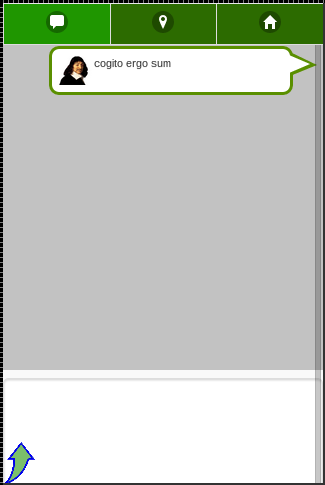
\includegraphics[scale=0.5]{bilder/screenshots/conference.png} & & 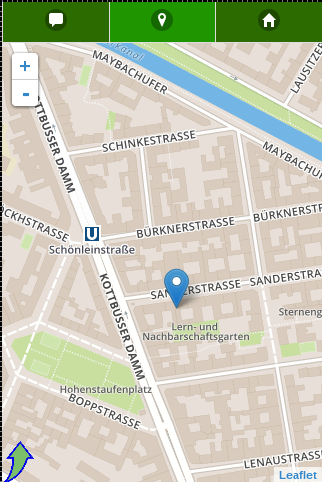
\includegraphics[scale=0.5]{bilder/screenshots/map.png} & & 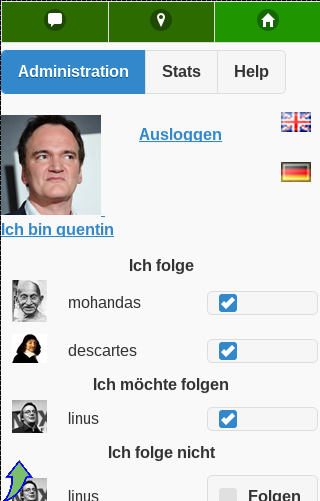
\includegraphics[scale=0.5]{bilder/screenshots/home.png} \\
			Conference & & Map & & Home
		\end{tabulary}
  		\end{adjustwidth}
	\end{table}
\noindent
Ein Klick auf den grünen Pfeil öffnet ein Kontext-Navigations-Fenster das wiederum aus 3 Ansichten besteht.
Jede dieser Ansichten beinhaltet Links zu Punkten auf der Karte und ermöglicht damit eine schnelle Kontext-bezogene Navigation:
\begin{itemize}[leftmargin=*,noitemsep,topsep=1ex,parsep=0pt,partopsep=0pt]
\item \textbf{Points-Of-Interest}: Hier werden alle POIs im angegebenen Umkreis angezeigt. 
\item \textbf{Bookmarked Locations}: Hier werden alle POIs und Locations angezeigt für die der Benutzer
ein Lesezeichen eingetragen hat.
\item \textbf{People Of Interest}: Hier werden alle entfernten Benutzer angezeigt, mit denen der lokale Benutzer eine Kontakt-Beziehung hält.
\end{itemize}
	
	\begin{table}[H]
  		\begin{adjustwidth}{-0.3cm}{0.3cm}
		\centering
		\begin{tabulary}{\columnwidth}{C >{\centering}m{1cm} C >{\centering}m{1cm} C}
			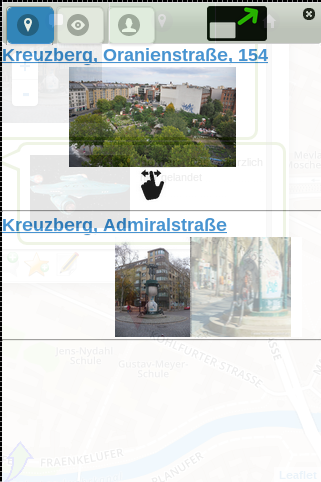
\includegraphics[scale=0.5]{bilder/screenshots/context_nav_pois.png} & & 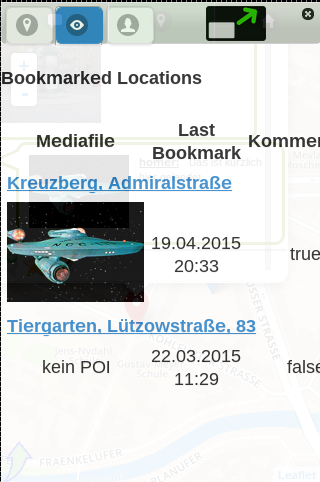
\includegraphics[scale=0.5]{bilder/screenshots/context_nav_bookmarks.png} & & 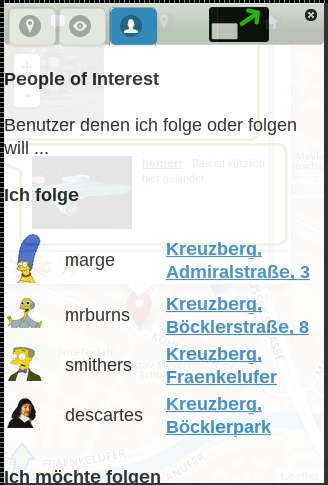
\includegraphics[scale=0.5]{bilder/screenshots/context_nav_contacts.png} \\
			Points of Interest & & Bookmarks & & People of Interest
		\end{tabulary}
  		\end{adjustwidth}
	\end{table}

\subsubsection{Registrierung \& Login}

\paragraph{Registrierung}
Zur vollen Nutzung der Anwendung muß ein Benutzer vom System authentisiert sein. Es gibt 2 Möglichkeiten sich 
zu registrieren:
\begin{itemize}
	\item Registrierung mit Email-Adresse und Passwort
	\item Registrierung mit einem Konto eines sozialen Netzwerks wie Facebook oder Twitter
\end{itemize}
\noindent Bei der Registrierung mit einem Passwort muss der Benutzer die Möglichkeit haben ein neues Passwort anzufordern wenn er nicht angemeldet ist. Das gilt nur bei einer Registrieung mit Email-Adresse und Passwort.

\paragraph{Login}
Eine Sitzung ist aus Sicherheitsgründen zeitlich begrenzt. Da sich ein Benutzer von jedem beliebigen Rechner einloggen kann muss verhindert werden, daß eine andere Person die authentisierte Sitzung eines Benutzers fortführt, falls letzterer die Sitzung nicht selbst durch eine aktive Abmeldung vom System beendet hat. 

\paragraph{Quick Registration}
Um es neuen Benutzern zu erleichtern das funktionale Angebot von VoyageX kennenzulernen und dennoch die registrierten 
Mitglieder der Community vor Störungen durch Aktivitäten unbekannter Nutzer zu schützen, wird eine Quick Registration angeboten, die eine volatile Collaborative Session ermöglicht (\cite[S. 72ff.]{SCLU:PFCMI}).
Bei dieser Form der Registrierung ist der Funktionsumfang der Anwendung allerdings eingschränkt.


\subsubsection{Community Support}
\paragraph{Gruppen}
TODO - Dieses Feature ist noch nicht programmiert - macht es Sinn? + wenn der Aufwand zu groß ist dann als TODO.\\
Gruppen können nur von Benutzern mit entsprechender Berechtigung angelegt werden. Um einer Gruppe beitreten zu können
benötigt ein Benutzer eine Einladung. Alle offenen Einladungen werden als Link in der Verwaltungs-Ansicht angezeigt.\\
Alle Interaktions-Funktionen der Anwendung sind auf die Mitglieder jener Gruppen beschränkt, für welche ein Benutzer eine Mitgliedschaft besitzt. Die Interaktion mit anderen Gruppenmitgliedern ist aber nicht verpflichtend - d.h. daß man anderen Gruppenmitgliedern nicht folgen muß.\\
%mit Gruppen macht auch eine user-gallery (siehe auch \cite[S. 72ff.]{SCLU:PFCMI}) mehr sinn - was bringt es alle mitglieder des gesamten systems zu sehen?
%(anders wenn bei der user-gallery interessen berücksichtigt werden die der benutzer irgendwo festgelehgt hat.)\\
Mögliche sinnvolle Erweiterung: Jede Gruppe hat ihre eigenen POIs.
%wenn ein poiu in 2 gruppen vorkommt muss man eine auswahl treffen, allerdings wird die ja auch in photonav angezeigt -serh komplex. etwas weniger komplex - alle haben poi - erster eintrag bei allen angezeigt aber die darber nur aus der gruppe.

\paragraph{Avatare}
Durch die Einführung von Avataren wird es für die Benutzer einfacher persönliche Kontakte auszuwählen und einen Überblick über ausgewählten Interaktionspartner zu wahren (siehe auch \cite[S. 97ff.]{SCLU:PFCMI}). Jeder Benutzer kann ein Bild (Foto oder Cartoon) wählen welches alle seine Beiträge und seinen Marker, sowie seine Präsenz in allen Listen schmückt. Jeder Benutzer hat eine Homebase.
%Jeder Benutzer hat mindestens eine Gruppe. und somit eine Zuordnung für andere Benutzer erleichtert wird.

\paragraph{Buddy List}
In VoyageX wählt man Kontakte, an denen man interessiert ist, über die "`Folgen"'-Beziehung.
%von benutzern aus diesen
%gruppen erhält man benachrichtigungen - soweit man dazu berechtigt ist.
%eine der buddy-list bvergleichbare liste wäre dann die liste der benutzer denen ich folgen will und darf, %erweitert um die liste der benutzer denen ich folgenwill aber noch nicht darf.


%\subsubsection{Verwendete Standards, 3rd Party Libs}
%\paragraph{Omniauth}
%omniauth ist ein rails gem das konfigurierbare authentisierungsmechanismen(strategien in omniauth) in form von plugins für viele verbreitete provider(facebook, twitter, ...) oder standards(ldap,..) bietet. fr neue provider können
%neue  strategie-plugins geschrieben werden die ohne änderung des anwendungs-codes eingebunden werden können.

%\paragraph{Avatare}
%zur verinfachung der avatar-einbindung wird die per email-addtesse defieierte bindung von gravatar angeboten - 
%falls der benutzer kein gravata-acount hat wird ein comic-ähnliches bold von einem japanischen hersteller gewäjlt

\subsection{Kartenbearbeitung}\label{5_KARBE}

\subsubsection{Initialisierung der Kartenansicht}\label{5_DARS_KART}
%Die Karten-Ansicht wird mit dem Map-Viewer von LeafletJS initialisiert.
Für die Initialisierung der Karten-Darstellung mit dem LeafletJS-Map-Viewer muß im Html-Quelltext der Seite zunächst ein mit einem frei wählbaren id-Attribut gekennzeichnetes Div-Element notiert werden, welches von Leaflet für die Einbindung der Karte genutzt werden kann.
\lstset{language=Html5}
\begin{lstlisting}[frame=single,numbers=none,xleftmargin=0pt]
<div id="map"></div>
\end{lstlisting}
Mit einem "`Options"'-Javascript-Objekt können dann weitere Konfigurations-Parameter übergeben werden, wobei die Parameter "`center"' (Kartenmittelpunkt) und "`zoom"' (Auflösung) obligatorisch für die Darstellung eines Kartenausschnittes in einem vorgegebenen Maßstab sind. In VoyageX wird beispielsweise
initiial das Zoom-Level 16 eingestellt und die Karte nach erfolgter Positions-Bestimmung des Clients durch die Browser-API-Funktion "`navigator.geolocation.getCurrentPosition"` um die aktuelle Position des Endgerätes zentriert.\\

\lstset{language=JavaScript}
\begin{lstlisting}[frame=single,xleftmargin=0pt,caption={Initialisierung der Karte in einer Haml-Datei},captionpos=b]
= javascript_tag do
  ...
  var tileLayer = new L.TileLayer.Functional(VoyageX.MapControl.drawTile, ...)
  var mapOptions = { center: new L.LatLng(#{@lat}, #{@lng}),
   				   	 zooms: [1,2,...,16],
   				   	 zoom: 16,
   				   	 subdomains: ['a'],
   				   	 access_token: 'pk.eyJ1I...ZiG5HGi5JAb64G1K-jA',
   				   	 layers: [tileLayer] }
  new L.Map('map', mapOptions)
\end{lstlisting} \vspace{0.8cm}

\noindent Wie in \ref{LEAFL} bereits beschrieben, macht Leaflet keine Vorgaben zum Darstellungs-Inhalt sondern benötigt nur die Urls der Kacheln aus denen die Karte zusammengesetzt werden soll. Leaflet berechnet dabei für jede Kachel des aktuell angezeigten Kartenabschittes den Koordinaten-Offset des oberen linken Kachelpunktes. Mit diesem x/y-Wert und dem aktuell eingestellten Zoom-Level z kann man alle für die Anzeige benötigten Kacheln identifizieren, und dann von einem Tile-Service unter Urls nach dem (Beispiel-)Muster 
\lstset{language=JavaScript}
\begin{lstlisting}[frame=single,numbers=none,xleftmargin=0pt]
http://a.tiles.mapbox.com/v4/stephankoeller.k5hhdli3/{z}/{x}/{y}.png
\end{lstlisting}%
laden.\\

\subsubsection{Darstellungs-Elemente}
VoyageX bietet eine Desktop-Version und eine mobile Version der funktional identischen graphischen Benutzeroberfläche des Clients, um die plattform-spezifischen Darstellungs-Parameter zu berücksichtigen.
Die Unterschiede  der Ansicht sind aber wegen der überschaubaren Funktionalität gering.

\begin{table}[H]
  \begin{adjustwidth}{-0.7cm}{0.7cm}
  \begin{tabulary}{\columnwidth}{ c c }
	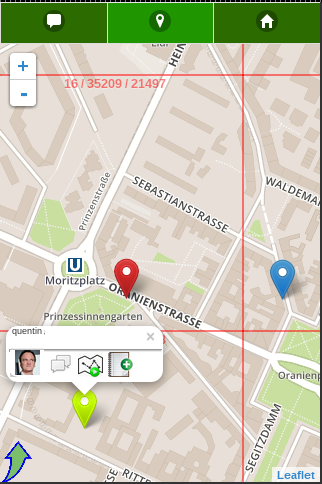
\includegraphics[scale=0.6]{bilder/screenshots/map_mobile.png} & 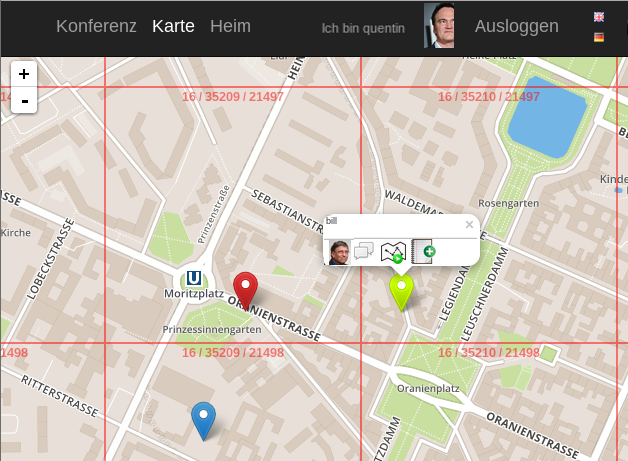
\includegraphics[scale=0.62]{bilder/screenshots/map_desktop.png} \\
	Mobiler Client & Desktop Client \\
% TODO with colspan 2. Die Kacheln sind rot umrandet und mit x/y/z-Angaben versehen
  \end{tabulary}
  \end{adjustwidth}
  \caption{Karten-Darstellung in VoyageX}
\end{table}



\paragraph{Marker}
Mit Markern werden feste und bewegliche Punkte auf der Karte gekennzeichnet. Alle Marker können in einem Popup ein Kontext-spezifisches Werkzeugmenu anzeigen. In VoyageX gibt es 3 Marker-Typen:
\begin{itemize}[leftmargin=*,noitemsep,topsep=1ex,parsep=0pt,partopsep=0pt]
\item 
\includegraphics[scale=0.3]{bilder/marker-icon-blue.png} \textbf{Arbeitsmarker}: Mit der Positionierung dieses Markers wird ein Punkt auf der Karte ausgewählt, den der Benutzer bearbeiten möchte. Die Positionierung kann automatisch über die GPS-Standortbestimmung, oder manuell mit einem Klick auf die Karte durchgeführt werden. Es gibt nur einen Arbeitsmarker pro Client.
\item 
\includegraphics[scale=0.3]{bilder/marker-icon-red.png} \textbf{POI-Marker}: Kennzeichnen Points of Interest (POI), also Orte oder Objekte. Die Anzahl der POIs ist nicht begrenzt, es wäre aber sinnvoll die Anzeige, wie bei anderen Location-Based-Apps durch Filter einzugrenzen, welche durch eine Suchfunktion definiert werden könnten. Im Rahmen dieser Arbeit wurde auf dieses Feature aufgrund des nötigen Aufwands
verzichtet.
\item 
\includegraphics[scale=0.3]{bilder/marker-icon-yellow.png} \textbf{Peer-Marker}: Mit diesen Markern werden Positionen von den entfernten Arbeitsmarkern anderer Benutzer angezeigt. Voraussetzung dafür ist eine Erlaubnis des jeweiligen entfernten Benutzers (Peer). Die Position kann dabei durch folgende Modi bestimmt sein:
	\begin{itemize}
		\item Der Marker zeigt den aktuell per GPS bestimmten Standoort des entfernten Benutzers
		\item Der Marker zeigt die manuell festgelegte Position des entfernten Arbeistmarkers. In diesem Modus kann ein Benutzer den entfernten, ihm zugeordneten Peer-Marker mit seinem lokalen Arbeitsmarker steuern. Dabei kann er wie in dd beschrieben Pfade auf dem entfernten Rechner zeichnen.
	\end{itemize}
\end{itemize}

\subsubsection{Bearbeitungsfunktionen}
Das Werkzeugmenu eines Markers wird durch Mouseover oder Klicken auf den Marker geöffnet.

\paragraph{Arbeitsmarker}
Mit dem Arbeitsmarker können Funktionen und Einstellungen zur Kartenbearbeitung aufgerufen werden.

  \begin{figure}[H]
      \centering
	  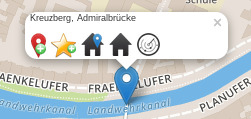
\includegraphics[scale=0.8]{bilder/screenshots/menu_arbeitsmarker.png}\\ 
  	  \caption{Werkzeugmenu des Arbeitsmarkers}
  \end{figure}

\begin{itemize}[leftmargin=*,noitemsep,topsep=1ex,parsep=0pt,partopsep=0pt]
\item 
\includegraphics[scale=0.55]{bilder/icons/add-marker.png} \textbf{POI eintragen}: Öffnet das Eingabeformular für POIs an der aktuellen Marker-Position. Neben einer obligatorischen textuellen Beschreibnung des POIs muss der Typ des Anhangs ausgewählt werden. 4 Typen stehen zur Auswahl:
	\begin{itemize}[leftmargin=*,noitemsep,topsep=1ex,parsep=0pt,partopsep=0pt]
		\item \textbf{Plain Text}: Ein Plain-Text Eintrag hat keinen Anhang. Allerdings wird als Default Icon ein weisses Rauschen angezeigt. Dies motiviert den Benutzer dann vielleicht doch einen aussagekräftigeren Anhang zu wählen.
		\item \textbf{Foto}: Falls verfügbar kann mit einer Kamera des Endgeräts ein Foto aufgenommen und angehängt werden. Bei mehreren Kameras muß der Benutzer eine Auswahl treffen.
		\item \textbf{Datei}: Vom lokalen Datei-System kann eine Bild-, Audio- oder Video.Datei hochgeladen werden.
		\item \textbf{Embed}: Embed sind Html-Code-Schnipsel mit denen Anhänge von externen Social-Media-Seiten wie Youtube oder Soundcloud eingebunden werden können. Einfache urls werden als Link zu einer Bild-Datei interpretiert.
	\end{itemize}
\item 
\includegraphics[scale=0.15]{bilder/icons/add-bookmark.png} \textbf{Lesezeichen}: Öffnet ein Textfeld für eine Notiz zur aktuellen Markerposition. Diese Daten sind für den persönlichen Gebrauch des Benutzers und werden nicht geteilt. Die gebookmarkten Orte müssen (noch) keine POIs sein, in der Kontext-Navigation wird die gesamte Leseliste angezeigt. Bookmarks unterstützen den Benutzer beim Navigieren, Planen und Ideen sammeln.
\item 
\includegraphics[scale=0.15]{bilder/icons/set-home.png} \textbf{Homebase markieren}: Markiert den aktuell ausgewählten Punkt um später schnell zu diesem "`zurückkehren"' zu können.
\item 
\includegraphics[scale=0.15]{bilder/icons/home.png} \textbf{Homebase anzeigen}: Karte auf Homebase zentrieren.
\item 
\includegraphics[scale=0.15]{bilder/icons/radar.png} \textbf{Radar}: Öffnet eine kontrollansicht zur Verwaltung des Kartenkontexts.
\end{itemize}

\begin{table}[H]
  %\begin{adjustwidth}{-2cm}{2cm}
  \begin{tabulary}{\columnwidth}{ C C C }
	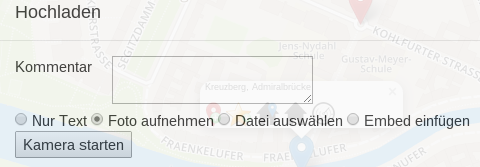
\includegraphics[scale=0.5]{bilder/screenshots/menu_arbeitsmarker_upload.png} &
	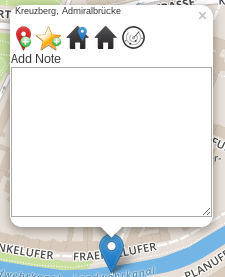
\includegraphics[scale=0.5]{bilder/screenshots/menu_arbeitsmarker_bookmark.png} &
	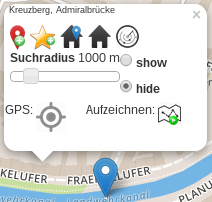
\includegraphics[scale=0.5]{bilder/screenshots/menu_arbeitsmarker_radar.png} \\
	
\includegraphics[scale=0.55]{bilder/icons/add-marker.png} &
	
\includegraphics[scale=0.15]{bilder/icons/add-bookmark.png} &
	
\includegraphics[scale=0.15]{bilder/icons/radar.png} \\
  \end{tabulary}
  %\end{adjustwidth}
  \caption{Weitere Schaltflächen}
\end{table}

\enlargethispage{2\baselineskip} % allow 3 more lines on current page
\paragraph{POI-Marker}
Mit dem POI-Marker können Funktionen und Einstellungen zur POI-Bearbeitung aufgerufen werden.

  \begin{figure}[H]
      \centering
	  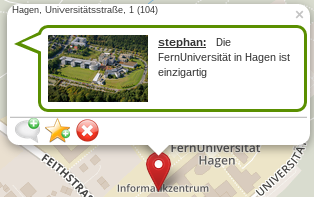
\includegraphics[scale=0.8]{bilder/screenshots/menu_poimarker.png}\\ 
  	  \caption{Werkzeugmenu des Arbeitsmarkers}
  \end{figure}

\begin{itemize}[leftmargin=*,noitemsep,topsep=1ex,parsep=0pt,partopsep=0pt]
\item 
\includegraphics[scale=0.15]{bilder/icons/add-comment.png} \textbf{Kommentieren}: Öffnet wie 
\includegraphics[scale=0.55]{bilder/icons/add-marker.png} das Eingabeformular für POIs für den ausgewählten POI - statt einen neuen POI zu erzeigen wird ein Kommentar an den existoerenden Poi angefügt. 
\item 
\includegraphics[scale=0.15]{bilder/icons/add-bookmark.png} \textbf{Lesezeichen}: Gleiche Funktion wie beim Arbeitsmarker.  
\item 
\includegraphics[scale=0.07]{bilder/icons/edit-note.png} \textbf{Notiz}: Wie beim Lesezeichen kann man eine Notiz mit der aktuellen Marker-Position assoziieren, diese wird aber nicht in der Kontext-Navigation als Lesezeichen angezeigt. Sie bezieht sich direkt auf den POI.
\end{itemize}

\subsection{Offline Funktionalität}\label{5_OFFL}
Die Anforderung zum Erhalt der Funktionsfähigkeit bei fehlender Netzwerkverbindung erfordert Lösungen für folgende Problembereiche:
\begin{itemize}
	\item Ausführbarkeit der Anwendung im Offline-Modus
	\item Vorladen der Kartenkacheln
	\item Lokales speichern der Bearbeitungs- und Kommunikationsdaten-Daten
\end{itemize}
\vspace{1ex}\noindent
Für die Synchronisation der Systemdaten müssen folgende Probleme gelöst werden:
\begin{itemize}
	\item Erstellen von IDs zur systemweit eindeutigen Identifikation lokal erzeugter Objekte
	\item Nebenläufigkeitsprobleme bei der Datensynchronisation
	\item Versionierung des Systemzustandes zur Synchronisation lokaler Kopien
\end{itemize}

\subsubsection{Ausführbarkeit der Anwendung im Offline-Modus}
Webseiten-Inhalte werden von einem Browser zwar gecached, allerdings gehen die geladenen Daten je nach Cache-Strategie in der Regel spätestens beim Beenden des Browsers verloren. Um die von einer Webseite geladenen Resourcen über einen Browser-Neustart persistent zu machen wird die in Html5 standardisierte Application-Cache-Schnittstelle genutzt. Dazu wird im Html-Tag über das Attribut \texttt{manifest} eine Datei referenziert, in der alle für die Client-Anwendung benötigten Resourcen (Assets) gelistet sind.
\lstset{language=Html}
\begin{lstlisting}[frame=single,numbers=none,xleftmargin=0pt]
<html manifest="voyagex.mf">
\end{lstlisting}%
Der Browser speichert diese dann dauerhaft, so daß sie, unabhängig von Netzwerkverbindung oder zwischenzeitlichen Neustarts, in der Anwendung verfügbar sind.\\
Um dynamische Inhalte, wie etwa neue POI-Einträge, im Offline-Modus darzustellen, müssen die entsprechenden Ansichten, wie in Abschnitt \ref{5_SPI} beschrieben, client-seitig aus Templates generiert werden.\\
%In VoyageX wird aufgrund der Einfacheit kein Template-Framework 
Dazu werden die Templates in die Hauptseite unsichtbar eingebunden und von der Coffee-Klasse  \texttt{VoyageX.TemplateHelper} für die Erzeugung der Ansichten verwendet.\\ \\
Ein POI-Popup:
\lstset{language=Javascript}
\begin{lstlisting}[frame=single,numbers=none,xleftmargin=0pt]
@openPOINotePopup: (poi, marker) ->
  popupHtml = TemplateHelper.poiNotePopupHtml(poi)
  marker.getPopup().setContent(popupHtml)
  marker.openPopup()
\end{lstlisting}%
wird aus einem Template:
\lstset{language=Html}
\begin{lstlisting}[frame=single,numbers=none,xleftmargin=0pt]
<div id="tmpl_poi_notes_container" style="display: none;">
  <div tmpl-id="poi_notes_container" data-poiId="{poi_id}">
    {poi_notes}
  </div>
</div>
\end{lstlisting}%
in VoyageX.TemplateHelper dynamisch generiert:
\lstset{language=Javascript}
\begin{lstlisting}[frame=single,numbers=none,xleftmargin=0pt]
@poiNotePopupHtml: (poi) ->
  poiNotesHtml = ""
  for poiNote, i in poi.notes
    poiNotesHtml += poiNotePopupEntryHtml(poiNote, i)
  popupHtml = getTemplate("tmpl_poi_notes_container").
              replace(/\{poi_id\}/g, poi.id).
              replace(/\{poi_notes\}/, poiNotesHtml)
\end{lstlisting}%


\subsubsection{Vorladen der Kartenkacheln}
Für die Kartenbearbeitung auch ohne Internet-Verbindung müssen die Kartenkacheln 
lokal vorgehalten werden. Dabei ist die Begrenzung des verfügbaren Speicherplatzes zu berücksichtigen.

\paragraph{Anzeige lokal gespeicherter Kacheln im Map-Viewer}
Das LeafletJS-Plugin functionaltilelayer$^{\textbf{\ref{LEAFPLFTL}}}$
\addtocounter{footnote}{1}%
\footnotetext{\label{LEAFPLFTL}\href{https://github.com/ismyrnow/Leaflet.functionaltilelayer}{functionaltilelayer - https://github.com/ismyrnow/Leaflet.functionaltilelayer} von \href{https://github.com/ismyrnow}{Ishmael Smyrnow}; letzter Zugriff: 26.02.2015}%
bietet die Möglichkeit, Karten-Kacheln aus dem lokalen Cache zu laden.\\
Bei der Initialisierung der Karte wurde, wie in \ref{5_DARS_KART} beschrieben, an den Leaflet-Map-Viewer für die Darstellung der Tiles-Ebene eine Instanz des Leaflet.functionaltilelayer übergeben.\\
Leaflet ruft für jede zu ladende Kachel eine Funktion auf, welche diese Url aus dem (Tile-Service-Provider-Url)Template generiert und zurückgibt. An dieser Stelle fängt das Tile-Layer-Plugin den Aufruf ab und leitet
ihn an die Funktion weiter, deren Referenz dem Plugin selbst bei der Initialisierung übergeben wurde - für VoyageX also die Methode \texttt{drawTile} der Coffee-Klasse \texttt{VoyageX.MapControl}:
\lstset{language=CoffeeScript}
\begin{lstlisting}[frame=single,xleftmargin=0pt]
@drawTile: (view) ->
  storeKey = getTileKey([view.tile.column, view.tile.row, view.zoom])
  storedTileUrl = getStoredTileUrl storeKey
  unless storedTileUrl?
    storeTile view
  else
    storedTileUrl

@storeTile: (view) ->
  tileUrl = VoyageX.TILE_URL_TEMPLATE
            .replace('{z}', view.zoom)
            .replace('{y}', view.tile.row)
            .replace('{x}', view.tile.column)
            .replace('{s}', view.subdomain)
  if APP.isOnline()
    if view.zoom in @_offlineZooms
   	  tileUrl = _loadAndPrefetch [view.tile.column, view.tile.row, view.zoom]
    else
      _prefetchZoomLevels [view.tile.column, view.tile.row, view.zoom]
  else
    tileUrl = _notInCacheImage view.tile.column, view.tile.row, view.zoom
  tileUrl
\end{lstlisting}%
Die Interceptor-Methode wird für jede Kachel aufgerufen.\\
\begin{table}[H]
  \begin{tabulary}{\columnwidth}{>{\raggedleft}m{.5cm} L}
  \hline
1: & Als Parameter wird der Interceptor-Methode eine Datenstruktur übergeben aus welcher die x-,y- und z-Werte der zu ladenden Kachel gelesen werden können. \\ \hline
5: & Nachdem die Kachel noch nicht lokal gespeichert wurde, wird die Methode "`storeTile"' aufgerufen um die Kachel eventuell zu speichern. \\ \hline
16: & Im Online-Verbindungsstatus wird die Kachel nur dann lokal gespeichert, wenn das Zoom-Level für den Offline-Cache konfiguriert ist. Andernfalls wird für die aktuell abgefragte Kachel die Original-Url zurückgegeben. Allerdings werden in beiden Fällen die Kacheln für die über, als auch unter dem aktuellen Zoom-Level liegenden Offline-Cache-Zoom-Level vorgeladen. \\ \hline
21: & Falls keine Netzwerkverbindung besteht wird eine Platzhalter-Kachel generiert die dem Benutzer das Fehlen der Kachel im Cache anzeigt. \\ \hline
  \end{tabulary}
\end{table}
\enlargethispage{2\baselineskip} % allow 2 more lines on current page
%Falls keine Netzwerk-Verbindung verfügbar ist werden für nicht lokal gespeicherte Kachel-Bilder entsprechende
%Hinweise angezeigt.
%  \begin{figure}[H]
%      \centering
%	  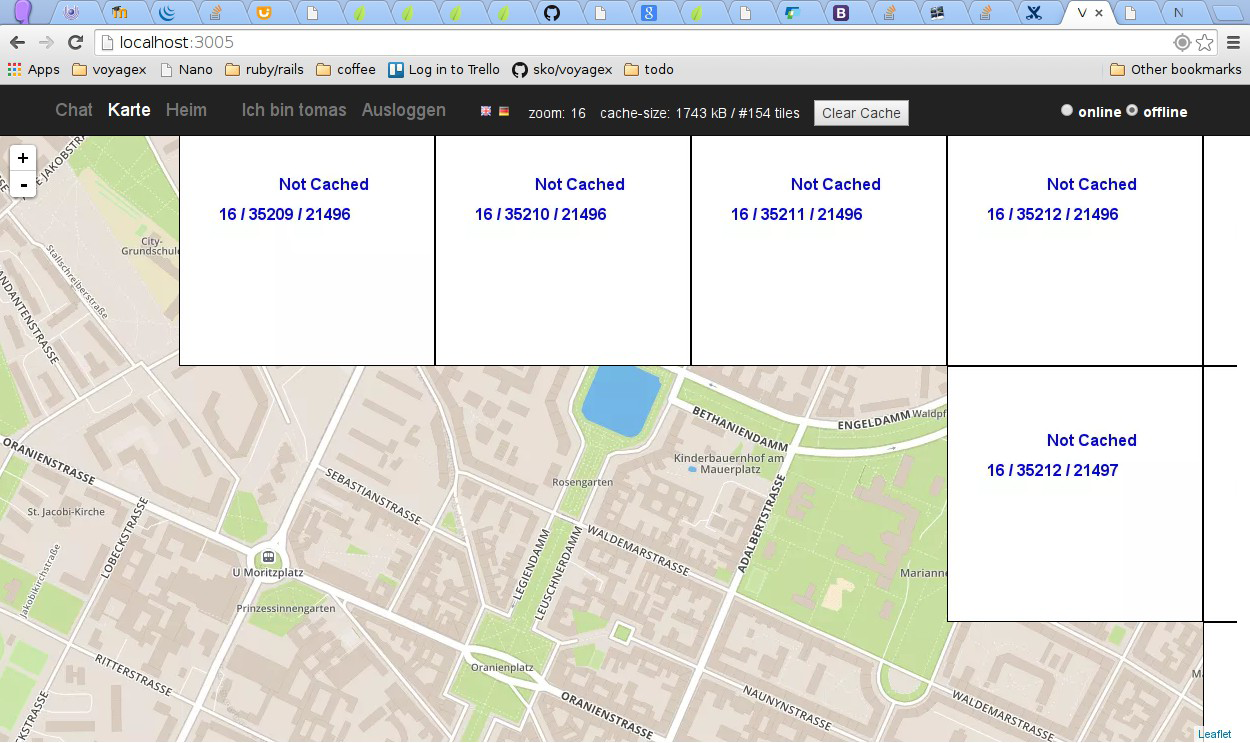
\includegraphics[scale=0.4]{bilder/map_offline.png}\\ 
%  	  \caption{Anzeige gespeicherter und fehlender Kacheln im Offline-Modus}
%  \end{figure}

\paragraph{Multithreaded File-Access: Promises$^{\textbf{\ref{CMTPROMISE}}}$}
\addtocounter{footnote}{1}%
\footnotetext{\label{CMTPROMISE}\href{http://www.html5rocks.com/en/tutorials/es6/promises/}{JS Promises - http://www.html5rocks.com/en/tutorials/es6/promises/}; letzter Zugriff: 26.02.2015}
%Der Map-Viewer generiert die Urls für die benötigten Kacheln, er kann aber nicht feststellen ob unter der Url tatsächlich eine Bild-Datei geladen werden kann. Wenn die Netzwerk-Verbindung abbricht während der Map-Viewer die Kachel-Bild-Urls bereits generiert und in den HTML-Dom-Baum eingebunden hat, dann werden die
Der Map-Viewer erwaret also beim Aufruf von \texttt{drawTile} eine Kachel-Url als Rückgabewert. Nun muß folgendes Problem für das Laden lokal gespeicherter Kachel-Bilder gelöst werden: Während Zugriffe auf localStorage synchron erfolgen können, bietet die File-API aber keine Möglichkeit zum synchronen Lesen oder Speichern von Dateien$^{\textbf{\ref{CMTASYNCIDB}}}$%
\addtocounter{footnote}{1}%
\footnotetext{\label{CMTASYNCIDB}An dieser Stelle sei noch angemerkt daß auch eine Client-seitige Persistenz-Implementierung mit IndexedDB in einem Multithreaded Kontext abläuft}. Deshalb gibt \texttt{drawTile} keine Urls sondern Javascript-\texttt{Promises} zurück$^{\textbf{\ref{CMTPROMFORLEAF}}}$%
\addtocounter{footnote}{1}%
\footnotetext{\label{CMTPROMFORLEAF}Die Möglichkeit zur Promise-Verarbeitung ist im Plugin bereits explizit implementiert}
%Damit die im Map-Viewer lokal gespeicherte Kachel-Bilder anzeigen kann gibt es 2 Möglichkeiten:
%\begin{itemize}
%\item Er lädt sie von Urls aus dem Netz und die Anwednung überschreibt 
%\item \textbf{Karte}: In dieser Ansicht werden die Karte sowie Navigations- und Steuerungs-Elemente angezeigt.
%\item \textbf{Heim}: In der Heimansicht befinden sich die Eingabe- und Steuerungs-Elemente zur Verwaltung der Benutzer- und Kontakt-Daten.
%\end{itemize}
%Der Map-Viewer soll im Offline-Modus lokal gespeicherte Kachel-Bilder anzeigen, 
%Für das Laden eines Bildes wird in Javascript ein neuer Thread gestartet. Allerdings erwartet 
%Damit der Map-Viewer auf die Bild-Daten dennoch wartet, erhält er eine Javascript-Promise.
%Um ein lokal gespeichertes Kachel-Bild anzuzeigen, muß der Map-Viewer auf die 
Im folgenden Code-Snippet wird gezeigt, wie die Bilddaten von einer Url geladen und lokal gespeichert werden.
\lstset{language=CoffeeScript}
\begin{lstlisting}[frame=single,xleftmargin=0pt]
loadReadyImage: (imgUrl, xYZ) ->
  deferred = $.Deferred()
  img = new Image
  img.onload = (event) ->
    base64ImgDataUrl = _toBase64 $('#tile_canvas')[0], this
    storeImage xYZ, base64ImgDataUrl
    deferred.resolve base64ImgDataUrl
  img.src = imgUrl
  return deferred.promise  
\end{lstlisting}%
\begin{table}[H]
  \begin{tabulary}{\columnwidth}{>{\raggedleft}m{.5cm} L}
  \hline
2: & Für das Laden des Bildes ein \texttt{deferred} Objekt erzeugt welches callback-Aufrufe einer \texttt{Promise} verwaltet \\ \hline
4: & Die Callback-Methode wird aufgerufen wenn die Bild-Datei vollständig geladen wurde. Die Bild-Daten werden dann auf einem Canvas-Objekt in eine base64-Data-Url konvertiert, die lokal gespeichert wird. Mit dieser Url wird dann die \texttt{Promise} eingelöst, also der Map-Viewer wird benachrichtigt daß er das Bild jetzt unter dieser (lokalen) Url laden soll.\\ \hline
9: & Die \texttt{Promise} wird anstatt einer echten Url zurückgegeben  \\ \hline
  \end{tabulary}
\end{table}
Im Map-Viewer wird unterdessen wie folgt auf die Bild-Url gewartet:
\lstset{language=CoffeeScript}
\begin{lstlisting}[frame=single,xleftmargin=0pt]
promise = loadReadyImage 'http://.../image.png', [13456,546,16]
promise.then (url) ->
  renderImage url
\end{lstlisting}
\vspace{2ex}
Im folgenden sind die Abläufe beim Laden und Speichern von Bildern in VoyageX dargestellt. Im synchronen Aufruf von \texttt{deferred} wird eine \texttt{Promise} zurückgegeben. Diese wird dann asynchron mit einer Data-Url einer bereits lokal gespeicherten oder einer erst zu ladenden und anschließend zu speichernden Datei aufgelöst.
%  webp - data-url
%functional-til-layer unterstützt aber javascript-promises, eine promis implementierz u.a. den calback then
%der aufgerufen wird sobald ein wert verfügbar ist.
%mit promises werden auch javascript new Image geladen.
%nahcdem de aufrufe nicht syncron hintereinander ausgeführt.
%wirk das seh komplex und man muss 
%und jetzt das sequenzdiagramm
%\enlargethispage{2\baselineskip} % allow 2 more lines on current page
  \begin{figure}[H]
      \centering
	  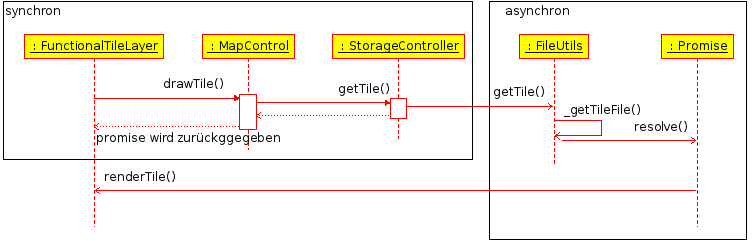
\includegraphics[scale=0.7]{bilder/uml/loadTile.png}\\ 
  	  \caption{Ladevorgang 1 - synchroner Aufruf von \texttt{getTile} und asynchrones Lesen einer Datei mit Auflösung der Promise}
  \end{figure}
  \begin{figure}[H]
      \centering
	  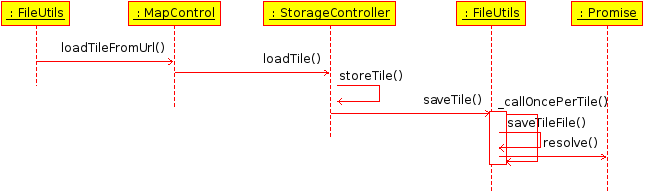
\includegraphics[scale=0.7]{bilder/uml/saveTile.png}\\ 
  	  \caption{Ladevorgang 2 - asynchrones Schreiben einer Datei mit Auflösung der Promise}
  \end{figure}

\paragraph{Vorladestrategien}
Beim Vorladen der Kacheln sollten für jede gecachte Kachel auch die darüberliegenden Kacheln für die gewünschten Offline-Zoom-Level vorgeladen werden, damit ein Benutzer auch in der niedrigsten Auflösung
den gecachten Bereich auf der Karte finden kann.
\enlargethispage{2\baselineskip} % allow 3 more lines on current page
	\begin{table}[H]
  		\begin{adjustwidth}{-0.3cm}{0.3cm}
		\centering
		\begin{tabulary}{\columnwidth}{C >{\centering}m{1cm} C >{\centering}m{1cm} C}
			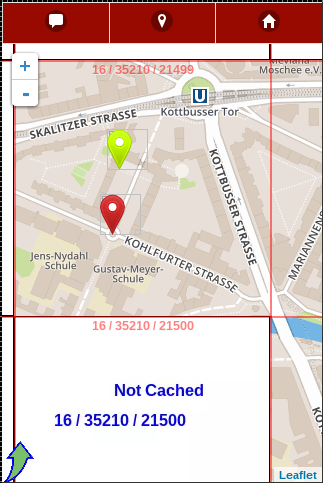
\includegraphics[scale=0.5]{bilder/screenshots/offline_16.png} & & 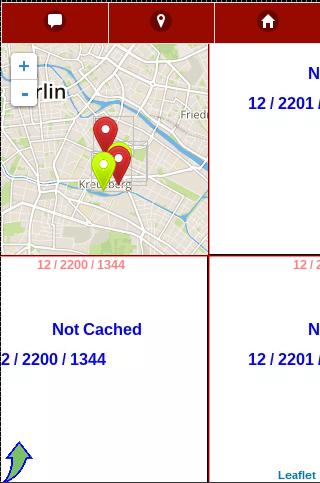
\includegraphics[scale=0.5]{bilder/screenshots/offline_12.png} & & 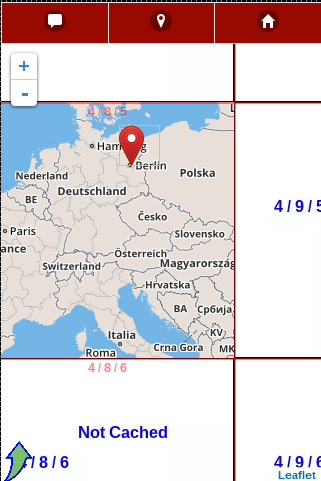
\includegraphics[scale=0.5]{bilder/screenshots/offline_4.png} \\
		\end{tabulary}
  		\end{adjustwidth}
	\end{table}
Für das Vorladen werden in VoyageX 2 Strategien implementiert:
\begin{itemize}[leftmargin=*,noitemsep,topsep=1ex,parsep=0pt,partopsep=0pt]
	\item \textbf{Umkreis um aktuellen Standort}: Bei dieser Strategie werden nach jeder Kartenverschiebung durch den Benutzer die Kacheln in einem einstellbaren Radius um den aktuellen Standort vorgeladen. Dabei werden wahrscheinlich auch viele unbenötigte Kacheln geladen - insbesondere wenn sich der Benutzer länger in eine bestimmte Richtung bewegt, und der Radius groß gewählt wurde.
	\item \textbf{Bewegungsrichtung}: Folgender sehr einfache Vorladealgorithmus, der die Bewegungsrichtung und die Geschwindigkeit berücksichtigt, wird von VoyageX implementiert:
	\begin{itemize}[leftmargin=*,noitemsep,topsep=1ex,parsep=0pt,partopsep=0pt]
%		\item
%		Die Grundidee ist folgende: Die Ungenauigkeit einer Messung der Bewegungsrichtung kann mit der Höhe der Geschwindigkeit wachsen.\\
%		Dazu folgende Algorithmus-Ausgangsfrage: Wenn der letzte, vor einer Stunde gemerkte Standort des Benutzers 100km in südlicher Richtung - vom aktuellen Standort betrachtet - war, dann wird er eine Stunde später 100km nördlich von der aktuellen Position sein. Falls der Benutzer allerdings vor 5 Minuten sein Ziel erreicht hat ist die Vorhersage sehr ungenau.\\
%		Die Idee für einen Algorithmus ist es jetzt, im Vorhersage-Algorithmus die Zeit-Abhängigkeit durch eine Entfernungs-Abhängigkeit ersetze - also nicht mehr wie im Beispiel jede Stunde zu messen, sondern ungefähr alle 100 Meter, wobei diese nicht exakt eingehalten werden müssen sondern, wie im folgenden ersichtlich wird, nur als Berechnungsgrundlage dienen.
%		\item Mit dem 100 Meter Richtwert wird zunächst jenes Zeit-Interval berechnet, in dem der Benutzer 100 Meter zurücklegt. Der Unterschied ist daß ich statt mit einem Wert "`100m / Zeiteinheit"` mit einem Wert
%		"`10min / Entfernungseinheit"` rechne. Da hat zur folge daß bei Steigender Geschwindigkeit öfters gemessen wird und die maximale Fehler-DIstanz die gewählte Entfernungseinheit ist.
%		\item Nach jeder Standort-Verschiebung wird also die nächste Position dann einfach als Verlängerung der Geraden (Luftlinie) von der zuletzt gemerkten Position über aktuelle Position um die gleiche Distanz berechnet. bei einer geschwindigkeit von 100 km/h wird  alle 0,001 stunden (3,6) sekunden  gemessen/veglichen.
%		bei 5 kmh also 0,08 stundrn alos alle 72 sekunden
		% bei 100kmg ich vergleiche also den standpunkt mit dem vor 3,6 sekunden
%		Die Kacheln werden dann entsprechend dem Radius in der richtung vorgeladen.
		\item Alle 100 Meter wird die Bewegunsrichtung bestimmt.
		\item Die Kacheln werden 1000 Meter in der Bewegungsrichtung vorgeladen
		\item Dazu wandert der Algorithmus horizontal bis zum Kachelende und dann vertikal bis zur Verbindungsgeraden zwischen Ausgangsort und vorhergesagter Position (1000m in aktuelle Richtung). Die gesuchten Kacheln sind all jene, deren Kanten$^{\textbf{\ref{CMTPATHALGO1}}}$
\addtocounter{footnote}{1}%
\footnotetext{\label{CMTPATHALGO1}1 bei Endkacheln , 2 bei Mittelkacheln} von der Verbindungsgeraden horizontal oder vertikal geschnitten werden, oder nur 1 Kachel falls Ausgangs- und Zielpunkt nah genug beieinander liegen.

  \begin{figure}[H]
  	\begin{adjustwidth}{-1cm}{1cm}
      \centering
	  \includegraphics[scale=0.6]{bilder/screenshots/move_prediction.png}\\ \vspace{0.8cm}
  	  \caption{Grün ist der zurückgelegte Weg, gelb der Weg zur vorhergesagten Position}
  	\end{adjustwidth}
  \end{figure}
		
	\end{itemize}
\end{itemize}

\subsubsection{Lokales Speichern von POI-Daten und Synchronisation}
Ein wesentliches Problem beim verteilten Erzeugen von Objekten ist die Vergabe von systemweiten IDs.\\
Es ist zwar möglich eine eindeutige ID zu erzeugen, beispielsweise könnte bei VoyageX ein lokal
erzeugtes POI-Objekt mit einem SHA-1 Hash aus Benutzer-ID und Timestamp systemweit eindeutig identifiziert werden. Allerdings hat die client-seitige Generierung von IDs einige Nachteile:
\begin{itemize}[leftmargin=*,noitemsep,topsep=1ex,parsep=0pt,partopsep=0pt]
\item Es entsteht dadurch eine externe Abhängigkeit des Systems von der gewählten Generierungs-Methode
\item Ein Mißbrauch durch manipulierte IDs kann ohne weitere Vorkehrungen nicht gänzlich ausgeschlossen werden.
\item Nachdem jeder POI nur einmal erzeugt werden soll muss für den Kollisionsfall Anwendungs-Logik entworfen werden welche die ID dann bei mindestens einem Benutzer korrigieren muss.
\end{itemize}
In klassischen Webanwendungen werden die Objekt-Daten an den Server gesendet wo sie erst zu einem Objekt gekapselt und mit einer ID versehen werden. Der Client erhält diese dann erst über die Response des Aufrufs.\\
Da für VoyageX die Anforderung nach Funktionalität im Offline-Betrieb aber voraussetzt, daß auch lokal erzeugte Objekte eindeutig identifiziert werden können, wird nun folgender Ablauf implementiert:
\begin{enumerate}[leftmargin=*,noitemsep,topsep=1ex,parsep=0pt,partopsep=0pt]
\item Das Objekt wird mit einer temporären lokalen ID gespeichert und in eine Upload-Queue geschrieben.
\item Sobald eine Verbindung zum Backend besteht werden alle Objekte in der  Upload-Queue hochgeladen. 
\item Im Backend werden die Objekte mit einer endgültigen systemweiten ID gespeichert, die dann zusammen mit der temporären an den Client zurückgeschickt wird
\item Im Client werden alle Elemente aus der Upload-Queue gelöscht und die ID vom Backend wird übernommen.
\end{enumerate}
%Wenn ein Benutzer den "`Sichern"'-Button im POI-Eingabeformular klickt werden die Daten zunächst lokal %gespeichert.
%\lstset{language=CoffeeScript}
%\begin{lstlisting}[frame=single,numbers=none,caption={Methode send der Coffee-Klasse Comm},captionpos=b]
%	$(document).on 'click', '#upload_button', (event) ->
%\end{lstlisting}
\enlargethispage{3\baselineskip} % allow 3 more lines on current page

\begin{table}[H]
  \begin{adjustwidth}{-1cm}{1cm}
  \begin{center}
  \begin{tabulary}{\columnwidth}{ c }
  \includegraphics[scale=0.8]{bilder/uml/queuePoiNote.png} \\
  \includegraphics[scale=0.6]{bilder/screenshots/queue_localStrorage_1.png}
  \end{tabulary}
  \caption{Eine POI-Notiz wird zuerst lokal gespeichert.}
  \end{center}
  \end{adjustwidth}
\end{table}
\noindent
Sobald der Client online ist (ggf. sofort) wird die POI-Note-Queue zum Backend hochgeladen:
\begin{table}[H]
  \begin{adjustwidth}{-2cm}{2cm}
  \begin{center}
  \begin{tabulary}{\columnwidth}{ c }
  \includegraphics[scale=0.7]{bilder/uml/syncPoiNoteQueue.png} \\
  \includegraphics[scale=0.6]{bilder/screenshots/queue_localStrorage_2.png}
  \end{tabulary}
  \caption{Die lokalen Ids von Loacation, Poi und PoiNote werden im localStorage aktualisiert und die Queue wird gelöscht.}
  \end{center}
  \end{adjustwidth}
\end{table}
\noindent
Im Backend wird die Integration der Daten asynchron durchgeführt - bei komplexen Operationen kann im Falle einer synchronen Abarbeitung (zwischen Request und Response) die dadurch entstehende Serverlast der Webanwendung hoch genug sein, daß weitere Requests durch Timeouts teilweise blockiert werden. In VoyageX wird für die asynchrone Bearbeitung ein Resque-Job gestartet, und die lokale Masterkopie des Benutzers anschließend über eine System-Call aktulalisiert.

\paragraph{Versionierung und Nebenläufigkeit}
Synchrone kooperative Systeme erlauben es mehreren verteilten Benutzern zur gleichen Zeit am gemeinsamen Datensatz zu arbeiten. Dazu werden oft auch bei online-Anwendungen Objekte repliziert um die Anwendungs-Performance durch den Umgehung der Netzwerk-Latenz zu steigern. Bei VoyageX erhält jeder Benutzer
eine Kopie der für ihn relevanten Systemdaten, also für jene Daten die in Bezug zu seinem lokalen Kartenausschnitt stehen. Eine Aktualisierung der Daten wird durch 2 Ereigisse ausgelöst:
\begin{itemize}[leftmargin=*,noitemsep,topsep=1ex,parsep=0pt,partopsep=0pt]
\item Der Client des Benutzers wird im online-Modus per System-Calls über Aktualisierungen durch andere Benutzer informiert
\item  Der Client wechselt vom offline- in den online-Modus
\end{itemize}
Um festzustellen ob der Client eine Aktualisierung benötigt wird jeder System-Daten-Änderung eine Commit-Id zugeordnet - wobei eine Änderung auch mehrere Objekte umfassen kann. Der Client kann also die aktuelle System-Commit-Id mit seiner eigenen vergleichen, um die Notwendigkeit einer Aktualisierung festzustellen.\\ \\ 
Die Versionierung der System-Daten wird über einem Git-Repository verwaltet. Dabei gibt es 2 Möglichkeiten, wie Client-Replikationen mit dem System-Master-Branch interagieren:
\begin{itemize}[leftmargin=*,noitemsep,topsep=1ex,parsep=0pt,partopsep=0pt]
\item für jeden Client wird ein eigenes Repository im Backend angelegt
\item für jeden Client wird ein Branch in einem Arbeits-Repository im Backend angelegt
\end{itemize}
Die zweite Methode ist wesentlich Resourcen-schonender und wir deshalb für VoyageX gewählt.\\
Wenn ein Client synchronisiert wird nur ein temporäres Arbeits-Verzeichnis mit dem aktuellen Commit des Clients angelegt. Mit einem \texttt{diff} werden die Änderungen analysiert und anschließend zusammengeführt.
Alle online-Clients erhalten eine Systembenachrichtigung, offline-Clients werden im Rahmen ihres nächsten Synchronisations-Request benachrichtigt.
%auf diese art wird der client über änderungen informiert die ihn aber vielleicht gart nicht betreffen weil
%die änderungen ausserhalb seines kartenausschnitts sind. andererseitsmuß das auch nicht zwangsläufig ein ausschlusskriterium sein denn der benutzer könnte sich ja in naher zukunft doch auch in dem bereicht aufhalten. es gibt auch verscheidene strageien die eine sinnvolle synchronisation haben kann. es wäre auch denkbar nach interessen oder gruppen-zugehörigkiet daten auszuwählen.

\subsubsection{Lokales speichern von Kommunikationsdaten-Daten}
Für die Speicherung von Kommunikations-Daten gilt folgendes:
\begin{itemize}[leftmargin=*,noitemsep,topsep=1ex,parsep=0pt,partopsep=0pt]
\item Nachrichten können nachträglich nicht geändert werden
\item P2P-Chat-Nachrichten werden nur lokal gespeichert. Die Sortierung kann bei verschiedenen Clients variieren.
\item Conference-Chat-Nachrichten erhalten einen Backend-System-Timestamp wenn sie am Kommunikations-Server eintreffen und werden direkt an alle Empfänger weitergeleitet. Die Sortierung kann bei verschiedenen Clients variieren.
\end{itemize}
 

%%%%%%%%%%%%%%%%%%%%%%%%%%%%%%%%%%%%%%%%%%%%%%%%%%%%%%%%%%%%%%
% Interaktion
%%%%%%%%%%%%%%%%%%%%%%%%%%%%%%%%%%%%%%%%%%%%%%%%%%%%%%%%%%%%%%

\subsection{Interaktion}\label{5_INTER}
Aus Interaktion-Teilnehmer-Sicht gibt es in VoyageX folgende 2 Formen der Interaktion:
\begin{itemize}
	\item Benutzer (User) - System
	\item Benutzer (User) - entfernter Benutzer (Peer)
\end{itemize}
Benutzer-System-Interaktion dient der Anwendungs-Steuerung. Der Nachrichten-Austausch zwischen Benutzern bedarf einer gegenseitigen Autorisierung. Jeder Benutzer muss selbst bestimmen (können), wer seine Aktionen verfolgen darf, und über wessen Aktionen er selbst informiert werden möchte. Beispiele für Benutzer-Benutzer-Interaktionen sind:
\begin{itemize}
	\item Chat-Nachrichten austauschen
	\item Benachrichtigungen über neu erstellte Karten-Einträge (z.B. abgegebene Kommentare) teilen
	\item Geographischen Positions-Angaben von Benutzern teilen
	\item Darstellungs-Elemente in Karten von Peers steuern
\end{itemize}

\subsubsection{Kontakte}
In VoyageX wird nur ein einfaches Autorisierungs-Konzept implementiert, es gibt nur einen Berechtigungs-Status, der bei VoyageX über das \texttt{Follow}-Flag gesetzt wird. Ein User kann nur mit jenen Peers Peers interagieren, die ihm eine Follow-Berechtigung erteilt haben. Die Follow-Berechtigung wird folgendermaßen erworben:
\begin{enumerate}[leftmargin=*,noitemsep,topsep=1ex,parsep=0pt,partopsep=0pt]
\item Ein User sendet einen Follow-Request an einen Peer. 
\item Dieser wird, wenn oder sobald er online ist, akkustisch und/oder visuell auf die neue Anfrage hingewiesen und kann diese in seiner Administrations-Ansicht sofort oder auch später bearbeiten.
\item Der User wird, wenn oder sobald er online ist, ebenfalls akkustisch und/oder visuell über die Entscheidung des Peers informiert. 
\end{enumerate}
Eine Follow-Beziehung kann jederzeit von jedem der beiden Interaktions-Partner wieder beendet werden.

\subsubsection{Initialisierung der Kommunikations-Infrastruktur}
Die 2-schichtige Kommunikations-Infrastruktur der VoyageX-Anwendung wird im Browser eines Benutzers über 2 Komponenten genutzt:
\begin{itemize}[leftmargin=*,noitemsep,topsep=1ex,parsep=0pt,partopsep=0pt]
\item \textbf{Transport:} Das Faye-Client-Script übernimmt die komplette Initialisierung der erforderlichen Netzwerk-Dienste:
	\begin{itemize}
		\item Aufbau und Verwaltung der Verbindung zum Server, Handshake, Wiederaufbau nach Unterbrechung, ...
		\item Transport der Nachrichten: Wahl des Transport-Protokolls und Routing
	\end{itemize}
\item \textbf{Anwendung:} Das VoyageX-Client-Script initialisiert und verwaltet die (logischen) Channels für einen Benutzer, die in 5 Typen unterteilt werden können:
%in Klammern steht die Angabe wie der Kanal vom Benutzer genutzt wird:
	\begin{itemize}
		\item eigener System-Channel: Über diesen Kanal werden Kontroll- und Status-Nachrichten zwischen System und Client ausgetauscht. (publish \& subscribe)
		\item eigener BC-Channel/Schlüssel: Öffentliche Nachrichten vom Benutzer. (publish)
		\item beliebig viele P2P-Channels/Schlüssel anderer Benutzer für private Nachrichten an diese Benutzer. (publish)
		\item eigener P2P-Channel: Private Nachrichten für den Benutzer. (subscribe)
		\item beliebig viele P2P-Channels anderer Benutzer für private Nachrichten an diese Benutzer. (subscribe)
	\end{itemize}
\end{itemize}

  \begin{figure}[H]
      \centering
	  \includegraphics[scale=0.5]{bilder/uml/register.png}
  	  \caption{Initialisierung der Kommunikations-Infrastruktur}
  \end{figure}


\subsubsection{Channels}
Alle Nachrichten werden als JSON-Objekte transportiert. Für die verschiedenen Interaktions-Formen werden folgende logischen Channels mit spezifischen Nachrichten-Formaten definiert.
\paragraph{/system}
System-Nachrichten informieren den Benutzer über:
\begin{itemize}
	\item Änderungen von Kontakt-Beziehungen
	\begin{itemize}
		\item Follow-Erlaubnis erhalten
		\item Follow-Erlaubnis abgelehnt
	\end{itemize}
\end{itemize}

  \begin{figure}[H]
      \centering
	  \includegraphics[scale=0.7]{bilder/uml/grantFollow.png}
  	  \caption{Benachrichtigung über die Publish-Subscribe-Infrastruktur am Beispiel einer Follow-Erlaubnis}
  \end{figure}

\paragraph{/talk}
	\begin{itemize}
		\item Konferenz-Chat Nachrichten
		\item P2P-Chat Nachrichten
	\end{itemize}

\paragraph{/pois}
	\begin{itemize}
		\item Neue POI-Einträge und Änderungen
	\end{itemize}

\paragraph{/radar}
	\begin{itemize}
		\item Peer-Positions-Angaben und -Änderungen
	\end{itemize}

\subsubsection{Anzeige entfernter Kontakte - Peer-Marker}
Kontakte werden auf der Karte mit einem Peer-Marker angezeit. Um Interaktions-Funktionen aufzurufen oder -Einstellungen zu ändern, kann per Maus-Klick ein Menu über dem Peer-Marker geöffnet werden.

  \begin{figure}[H]
      \centering
	  \includegraphics[scale=0.8]{bilder/screenshots/menu_peermarker.png}\\ 
  	  \caption{Menu des Peer-Markers}
  \end{figure}

\begin{itemize}[leftmargin=*,noitemsep,topsep=1ex,parsep=0pt,partopsep=0pt]
\item \includegraphics[scale=1.1]{bilder/icons/p2p-chat.png} \textbf{Chat}: Öffnet ein Dialog-Fenster für die Instant-Messaging-Kommunikation/Chat mit dem entfernten Benutzer. 
\item \includegraphics[scale=0.04]{bilder/icons/start_trace.png} \textbf{Trace}: Startet die Aufzeichnung der Positions-Änderungen des entfernten Arbeitsmarkers für passiven oder aktiven Trace.
\item \includegraphics[scale=0.07]{bilder/icons/edit-note.png} \textbf{Notiz}: Wie bei der POI-Notiz kann man hiermit Informationen über den Peer speichern.
\end{itemize}

\subsubsection{Kontakte lokalisieren}
Zu allen autorisierten Kontakten kann ein Benutzer den zuletzt bekannten oder aktuellen Aufenthaltsort auf der Karte anzeigen lassen. Dazu klickt man in der Administrations auf das Avatar-Bild des Peers. In der Kontext-Navigation werden in der Ansicht \texttt{People Of Interest} nur die Kontakte des aktuell definierten Such-Umkreises angezeigt.\\ \\
%In Abschnitt  
%Die Interaktions-Funktionen können über das Menu des Peer
%für interktionen mit einem kontat mus der marker des kontaktes lokalsiert werden es wäre zwar auch möglich
%interaktion wie p2pchat über die admin-maske zu starten - in voyagex ist das aber nun mal si.
%allerdings kann man über die adminmaske den marker aufrufen
%. darin werdne alle kontakte mit dem zuletzt von ihnen veröffentlichtem aufenthalts ort gelistet. über eine link kann man den enstprechned
Eine weitere Interaktions-Funktion zwischen Benutzern ist die dynamische Lokalisierung mittels \texttt{Trace} (Aufzeichnen von Pfaden). Ein Benutzer kann dabei mit Hilfe von GPS oder anderen Ortungsmethoden seine Position an andere User bekanntmachen.
Neben dem Chat gibt es noch eine weitere Funktion zur direkten Interaktion zwischen Benutzern: Trace (Aufzeichnen von Pfaden).
Beim Trace werden 2 Arten unterschieden.
\begin{itemize}
	\item \textbf{aktiv}: Ein User kann einem entfernten Benutzer (Peer) ermöglichen, den Peer-Marker auf der Karte des Users zu bewegen. Damit könnte ein Peer dem User Routen-Vorschläge machen.
	\item \textbf{passiv}: Ein User kann die GPS-Spur eines Peers, oder aber auch seine eigene, auf der lokalen Karte verfolgen.
\end{itemize}
\enlargethispage{3\baselineskip} % allow 3 more lines on current page
\begin{table}[H]
\begin{adjustwidth}{-1.5cm}{1.5cm}
\begin{center}
  \begin{tabulary}{20cm}{ C C C }
  	\includegraphics[scale=0.45]{bilder/screenshots/watch_peer_pos.png} &  & \includegraphics[scale=0.35]{bilder/screenshots/watch_my_pos.png} \\
  	s.koeller traced bert & & bert traced sich selbst \\
  \end{tabulary}
  \caption{Passiver Trace bei User und Peer}
\end{center}
\end{adjustwidth}
\end{table}

\subsubsection{Nachrichtenaustausch}
Die Infrastruktur für die Interaktion wird mit einem Publish-Subscribe-Messaging (PSM) System realisiert. Dabei werden für die Kommunikation logische Kanäle (Channels) definiert. Für den Empfang von Nachrichten wird ein Channel abonniert (subscribe), zum Versenden werden Nachrichten in einen Channel geschrieben (publish).\\ Für die Umsetzung der Kommunikations-Anforderungen in VoyageX müssen 2 Arten von Verbindungen bereitgestellt werden:
\begin{itemize}[leftmargin=*,noitemsep,topsep=1ex,parsep=0pt,partopsep=0pt]
\item \textbf{Broadcast (BC):}
	\begin{itemize}
		\item Jedem Benutzer ist eine BC-Verbindung zugeordnet. Nachrichten an mehrere Empfänger werden vom VoyageX-Client in den von autorisierten Peers abonnierten Broadcast-Kanal des Benutzers geschrieben. Der Kommunikations-Server blockiert in diesem Kanal Nachrichten die von Clients anderer Benutzer gesendet werden.
		\item Das System veröffentlicht Nachrichten die alle Benutzer erhalten sollen, beispielsweise Synchronisations-Benachrichtigungen, in einem allgemeinen System-Kanal.
	\end{itemize}

\item \textbf{Peer-To-Peer (P2P)}: 
	\begin{itemize}
		\item Jedem Benutzer ist ein P2P-Kanal zugeordnet. Für das versenden von Nachrichten an einen einzelnen Empfänger werden diese vom VoyageX-Client des Senders in den P2P-Kanal des Empfängers geschrieben. Der Empfänger ist der einzige Abonnent dieses Kanals, der Kommunikations-Server blockiert Abonnements von anderen Benutzern.
		\item Für den Empfang privater Nachrichten abonniert jeder VoyageX-Client für seinen Benutzer einen P2P-Kanal.
		\item Eine Sonderform eines P2P-Kanlals ist der benutzergebundene System-Kanal. Für jeden Benutzer wird genau ein
Systemkanal definiert, den nur der Client des Benutzers und der Server abonnieren, und in den nur diese beiden schreiben. Er ist also, im Gegensatz zu den anderen P2P-Channels bidirektional.
	\end{itemize}
\end{itemize}
Alle Kanäle haben eine Benutzer-spezifische Kennzeichnung. Zusätzlich können sie bei Bedarf verschlüsselt werden.

	%\multicolumn{2}{C}{} \\
%\begin{table}[H]
%  \begin{tabulary}{\columnwidth}{ C  C }
%	/talk@a3ri7vxl5 & /talk@a3ri7vxl5\_p2p \\
%	\multicolumn{2}{>{\centering}m{2.65cm}}{\includegraphics[scale=0.5]{bilder/ps_infrastructure.png}} \\
%	(BC) & (P2P)
%  \end{tabulary}
%  \caption{Beispiele für die beiden Kanäle eines Benutzers}
%\end{table}
\enlargethispage{3\baselineskip} % allow 3 more lines on current page

  \begin{figure}[H]
      \centering
	  \includegraphics[scale=0.5]{bilder/ps_infrastructure.png}\\ 
  	  \caption{Der BC- und der P2P-Kanal eines Benutzers}
  \end{figure}

  \begin{figure}[H]
      \centering
	  \includegraphics[scale=0.5]{bilder/ps_infrastructure_sys_bc.png}\\ 
  	  \caption{Der allgemeine System-Kanal}
  \end{figure}

  \begin{figure}[H]
      \centering
	  \includegraphics[scale=0.5]{bilder/ps_infrastructure_2.png}\\ 
  	  \caption{Der System-Kanal eines Benutzers}
  \end{figure}

\noindent\\ Auf Basis dieser Infrastruktur bietet VoyageX folgende 3 Interaktions-Formen.
\begin{itemize}
	\item Personal Chat (Kommunikation)
	\item Group Chat (Kommunikation)
	\item Benachrichtigungen (Information)
\end{itemize}

%Für die Implementierung der Kommunikations-Schicht reichen also 
%\lstset{language=CoffeeScript}
%\begin{lstlisting}[frame=single,numbers=none,caption={Methode send der Coffee-Klasse Comm},captionpos=b]
%  send: (channel, message, peer = null) ->
%    unless Comm.channelCallBacksJSON[channel.substr(1)] == null or !systemReady or !APP.isOnline()
%      channelPath = channel
%      unless window.VoyageX.USE_GLOBAL_SUBSCRIBE
%        channelPath += VoyageX.PEER_CHANNEL_PREFIX +
%                       if peer? then peer.peerPort.channel_enc_key+'_p2p' else Comm.channelCallBacksJSON[channel.substr(1)].channel_enc_key
%      if message.cacheId?
%        delete message.cacheId
%      client.publish(channelPath, message)
%    else
%      if (Modernizr.localstorage)
%        unless message.cacheId?
%          console.log('caching publish to '+channel)
%          message.cacheId = Math.round(Math.random()*1000000)
%          cacheEntry = { channel: channel, message: message, peer: peer }
%          @_storageController.addToList('comm.publish', 'push', cacheEntry)
%      else
%        alert('This Browser Doesn\'t Support Local Storage so This Message will be lost if you quit the Browser')
%\end{lstlisting}


\paragraph{P2P-Chat}
Um den persönlichen Chat-Dialog zu starten klickt ein Benutzer in der Kartenansicht auf den Marker des gewünschten Chat-Partners. Der VoyageX-Client jedes Benutzers schreibgt dessen Nachricht in den P2P-Channel des Gesprächspartners und zeigt alle Nachrichten an die in den eigenen P2P-Channel geschriebne wurden. Über neue Nachrichten wird der Benutzer mit einem akkustischen Signal und/oder einem Popup-Fenster informiert.

	\begin{table}[H]
  		\begin{adjustwidth}{-0.3cm}{0.3cm}
		\centering
		\begin{tabulary}{\columnwidth}{C >{\centering}m{1cm} C >{\centering}m{1cm} C}
			\includegraphics[scale=0.5]{bilder/screenshots/p2p_chat_1.png} & & \includegraphics[scale=0.5]{bilder/screenshots/p2p_chat_2.png} & & \includegraphics[scale=0.5]{bilder/screenshots/p2p_chat_3.png} \\
			Conference & & Map & & Home
		\end{tabulary}
  		\end{adjustwidth}
	\end{table}

 
\paragraph{Konferenz-Chat}
In der Konferenz-Maske können mehrere Benutzer miteinander kommunizieren. Der VoyageX-Client schreibt die Nachrichten eines Benutzers in dessen BC-Channel und zeigt alle Nachrichten an die über einen abonnierten Kanal veröffentlicht wurden. Über neue Nachrichten wird der Benutzer mit einem akkustuischen Signal und/oder einem Popup-Fenster informiert.

\enlargethispage{3\baselineskip} % allow 3 more lines on current page
  \begin{figure}[H]
      \centering
	  \includegraphics[scale=0.6]{bilder/screenshots/conference_chat.png}\\ 
  \end{figure}

\newpage


%\subsection{Testing}
%\subsubsection{Backend}
%\subsubsection{Frontend}
%\paragraph{capybara}

\newpage
%%%%%%%%%%%%%%%%%%%%%%%%%%%%%%%%%%%%%%%%%%%%%%%%%%%%%%%%%%%%%%
%
% Kapitel 6: Fazit
%
%%%%%%%%%%%%%%%%%%%%%%%%%%%%%%%%%%%%%%%%%%%%%%%%%%%%%%%%%%%%%%
\section{Fazit}
Lorem ipsum ...
